\chapter{模型无关性}\label{ch:model-independence}


我们在本章中的目标是证明：\trInfinityCategories{}的理论在\trChangeOfModel{}之下
不变。这一结果的部分含义已在第 10 章中建立，在那里我们证明：本书中发展的诸%
\trInfinityCategory{}性概念会被诸\trCosmologicalBiequivalence{}保持、反射并
创造，而正是这些\trBiequivalence{}为我们提供了\trChangeOfModel{}\trFunctor。
但我们在此的目标是要建立一个更强的结论：关于\trInfinityCategories{}的诸陈述，
即便是以单个\trInfinityCosmos{}所特有的「解析」技巧证明的，也同样是\trModelIndependent{}
——只要这些陈述可以在一种合适的\trEquivalence{}不变语言中表述。第 12 章例示
了这一转移原理的种种应用。

我们对\trInfinityCategory{}论之\trModelIndependence{}的朴素探讨——例如命题
10.3.6 中列举的那些结果——其问题在于：它们是特设的，而且颇为烦冗。在 11.1 节
中，我们将追求一个更系统化的结果。我们回顾与一个\trInfinityCosmos{}相关联的
模的\trVirtualEquipment{}的构造，并解释它为何描述了一个适合证明基本%
\trInfinityCategory{}性概念之\trModelIndependence{}的语境。随后，我们在%
\cref{thm:biequivalence-of-virtual-equipments}中证明：一个\trCosmologicalBiequivalence{}诱导诸虚拟装备之间的一个%
\trBiequivalence，并从这一结果的视角出发，重访我们的若干特设的%
\trModelIndependence{}陈述。

非正式地，\cref{thm:biequivalence-of-virtual-equipments}意谓：任何能够被编码为模的\trVirtualEquipment{}之性质
的\trInfinityCategory{}性概念都是\trModelIndependent{}；诸虚拟装备之间的一个%
\trBiequivalence{}给出一种机制，使得用某一种\trInfinityCategory{}的模型证明
的结果得以借此转移到另一个模型。但是，一个关于\trInfinityCategories{}的陈述，
在已经以虚拟装备的语言表述之后，我们如何能确知它在诸虚拟装备的%
\trBiequivalence{}之下事实上不变呢？

在 Blanc [19]、Freyd [43]、Preller [92] 与 Cartmell [25] 的既有工作的基础上，
Makkai 一直在追寻数学的一种高阶范畴论基础。特别地，他的\emph{带依赖排序的一阶逻辑}%
（First-Order Logic with Dependent Sorts，FOLDS）[82]提供了一种形式语言，用以
书写关于有限维高阶范畴结构的数学语句。在 11.2 节中，我们勾勒 Makkai 的 FOLDS
框架背后的关键想法，并解释他的工作如何经特殊化而表明：任何以「2-范畴的语言」
写下的陈述，在 2-范畴之间的\trBiequivalence{}之下不变。

由于\trInfinityCategories{}作为对象栖居于一个无穷维\trCategory{}之中，Makkai
的理论是否适用于眼前的情形，并非一目了然。然而，本书的一个关键主题是：%
\trInfinityCategory{}论中相当可观的一部分可以在一个截断的有限维框架中发展：
此即模的\trVirtualEquipment{}。在 11.3 节中，我们改造 Makkai 的框架，以证明：
任何能够在「虚拟装备的语言」（我们将在一个精确的意义上定义这一语言）中表述
的陈述，都会给出一个关于\trInfinityCategories{}的\trModelIndependent{}陈述。

\providecommand{\Mod}{\mathbb{M}od}
\providecommand{\Fun}{\operatorname{Fun}}
\providecommand{\HomA}{\mathrm{Hom}_{A}}
\providecommand{\HomB}{\mathrm{Hom}_{B}}
\providecommand{\Hom}{\mathrm{Hom}}

\section{虚拟装备的双等价}\label{sec:biequivalence-of-virtual-equipments}

在本节中，我们将证明：一个\trCosmologicalBiequivalence{}
$F\colon\mathcal{K}\Rightarrow\mathcal{L}$ 诱导诸虚拟装备之间的一个%
\emph{\trBiequivalence}
$F\colon\Mod(\mathcal{K})\Rightarrow\Mod(\mathcal{L})$。随后我们将解释这一结果
的含义：诸\trInfinityCategory{}的范畴论会被任何这种形式的「\trChangeOfModel{}」%
\trFunctor{}保持、反射并创造。

「诸\trInfinityCategory{}的理论是\trModelIndependent{}」这一主张无疑应当涵盖如下这样的
断言：
\begin{itemize}
\item 诸\trInfinityCategory{}之间的一个\trFunctor{}在一个特定的模型中拥有一个%
\trLeftAdjoint，当且仅当它在每一个模型中都拥有一个\trLeftAdjoint。
\item 一个以\trInfinityCategory{}为取值的\trDiagram{}在某个模型中拥有一个%
\trLimit，当且仅当它在每一个模型中都拥有一个\trLimit。
\end{itemize}

在我们的设定中，诸如 \eqref{eq:four-model-cosmoi} 那样的诸\trChangeOfModel{}%
\trFunctor{}定义诸\trCosmologicalBiequivalence，或由之构成的之字形链。沿着这些
思路，10.3 节中发展出了一种证明诸\trInfinityCategory{}的基本范畴论之%
\trModelIndependence{}的特设方法，在那里我们观察到：在双等价的诸%
\trInfinityCosmos{}之间，∞-范畴性数据与性质的特设翻译如果需要的话，可以相对
机械地、以极其烦冗的细节给出。

对\trModelIndependence{}的一种更为系统化的进路，会利用诸\trInfinityCategory{}的
形式范畴论的那个最为全面的框架，即模的\trVirtualEquipment。我们简要回顾其本质
特征。请回忆第 8 章：一个\trInfinityCosmos{} $\mathcal{K}$ 中的模的%
\textbf{\trVirtualDoubleCategory} $\Mod(\mathcal{K})$ 由下列诸项构成：

\begin{itemize}
\item 一个由\textbf{对象}与\textbf{竖直箭头}构成的\trCategory，此处即诸%
\trInfinityCategory{}与诸\trInfinityFunctor，竖直地描绘；
\item 对任意一对对象 $A$、$B$，一个由\textbf{水平箭头} $A\xrightarrow{E}B$ 组成
的汇集，此处即从 $A$ 到 $B$ 的诸\trModule{} $(q,p)\colon E\twoheadrightarrow A\times B$；
\item 诸\textbf{\trCell}，其边界描绘如下
\begin{center}
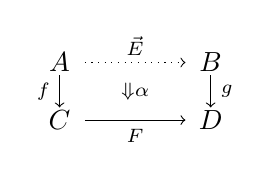
\begin{tikzpicture}[x=1.3em,y=1.3em]
  \node at (0,1.6) {$A$};
  \node at (4.2,1.6) {$B$};
  \draw[->,dotted] (0.7,1.6) -- (3.5,1.6);
  \node at (2.1,2.05) {$\scriptstyle\vec{E}$};
  \draw[->] (0,1.25) -- (0,0.35);
  \node at (-0.45,0.8) {$\scriptstyle f$};
  \draw[->] (4.2,1.25) -- (4.2,0.35);
  \node at (4.65,0.8) {$\scriptstyle g$};
  \node at (2.1,0.8) {$\scriptstyle\Downarrow\alpha$};
  \node at (0,0) {$C$};
  \node at (4.2,0) {$D$};
  \draw[->] (0.7,0) -- (3.5,0);
  \node at (2.1,-0.45) {$\scriptstyle F$};
\end{tikzpicture}
\end{center}
其中 $\vec{E}$ 是从 $A$ 到 $B$ 的一个模的相容序列
$E_{1}\divideontimes\cdots\divideontimes E_{n}$ 之缩写，在 $A=B$ 的情形下它可以
为空。此处，具有所示边界的一支\trCell{}是\trFunctorSpace{}
$\Fun_{f\times g}(\vec{E},F)$ 中对象的一个\trIsomorphism{}类，该空间由从双侧%
\trFibration{} $A\twoheadleftarrow\vec{E}\twoheadrightarrow B$ 到
$C\twoheadleftarrow F\twoheadrightarrow D$ 的、位于 $f\times g$ 之上的那些映射
构成；
\item 一支\textbf{复合}\trCell，对任何如下构型
\begin{center}
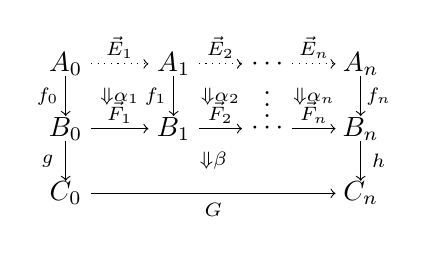
\begin{tikzpicture}[x=1.3em,y=1.3em]
  \node at (0,3.2)   {$A_{0}$};
  \node at (3.0,3.2) {$A_{1}$};
  \node at (5.6,3.2) {$\cdots$};
  \node at (8.2,3.2) {$A_{n}$};
  \draw[->,dotted] (0.7,3.2) -- (2.3,3.2);
  \node at (1.5,3.65) {$\scriptstyle\vec{E}_{1}$};
  \draw[->,dotted] (3.7,3.2) -- (4.9,3.2);
  \node at (4.3,3.65) {$\scriptstyle\vec{E}_{2}$};
  \draw[->,dotted] (6.3,3.2) -- (7.5,3.2);
  \node at (6.9,3.65) {$\scriptstyle\vec{E}_{n}$};
  \draw[->] (0,2.85) -- (0,1.75);
  \node at (-0.5,2.3) {$\scriptstyle f_{0}$};
  \draw[->] (3.0,2.85) -- (3.0,1.75);
  \node at (2.5,2.3) {$\scriptstyle f_{1}$};
  \node at (5.6,2.3) {$\vdots$};
  \draw[->] (8.2,2.85) -- (8.2,1.75);
  \node at (8.7,2.3) {$\scriptstyle f_{n}$};
  \node at (1.5,2.3) {$\scriptstyle\Downarrow\alpha_{1}$};
  \node at (4.3,2.3) {$\scriptstyle\Downarrow\alpha_{2}$};
  \node at (6.9,2.3) {$\scriptstyle\Downarrow\alpha_{n}$};
  \node at (0,1.4)   {$B_{0}$};
  \node at (3.0,1.4) {$B_{1}$};
  \node at (5.6,1.4) {$\cdots$};
  \node at (8.2,1.4) {$B_{n}$};
  \draw[->] (0.7,1.4) -- (2.3,1.4);
  \node at (1.5,1.85) {$\scriptstyle\vec{F}_{1}$};
  \draw[->] (3.7,1.4) -- (4.9,1.4);
  \node at (4.3,1.85) {$\scriptstyle\vec{F}_{2}$};
  \draw[->] (6.3,1.4) -- (7.5,1.4);
  \node at (6.9,1.85) {$\scriptstyle\vec{F}_{n}$};
  \draw[->] (0,1.05) -- (0,-0.05);
  \node at (-0.5,0.5) {$\scriptstyle g$};
  \draw[->] (8.2,1.05) -- (8.2,-0.05);
  \node at (8.7,0.5) {$\scriptstyle h$};
  \node at (4.1,0.5) {$\scriptstyle\Downarrow\beta$};
  \node at (0,-0.4)  {$C_{0}$};
  \node at (8.2,-0.4){$C_{n}$};
  \draw[->] (0.7,-0.4) -- (7.5,-0.4);
  \node at (4.1,-0.85) {$\scriptstyle G$};
\end{tikzpicture}
\end{center}
它由先拉回、随后复合诸跨度之映射的\trFiberedIsomorphism{}类而定义；
\item 一支\textbf{恒同}\trCell，对每一支水平箭头
\begin{center}
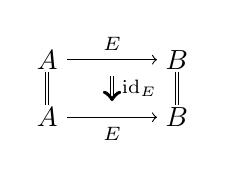
\begin{tikzpicture}[x=1.3em,y=1.3em]
  \node at (0,1.6) {$A$};
  \node at (3.6,1.6) {$B$};
  \node at (0,0) {$A$};
  \node at (3.6,0) {$B$};
  \draw[->] (0.55,1.6) -- (3.05,1.6);
  \node at (1.8,2.05) {$\scriptstyle E$};
  \draw[double,double distance=0.6pt] (0,1.25) -- (0,0.35);
  \draw[double,double distance=0.6pt] (3.6,1.25) -- (3.6,0.35);
  \draw[double,->] (1.8,1.15) -- node[right]{$\scriptstyle\mathrm{id}_{E}$} (1.8,0.45);
  \draw[->] (0.55,0) -- (3.05,0);
  \node at (1.8,-0.45) {$\scriptstyle E$};
\end{tikzpicture}
\end{center}
\end{itemize}
使得诸\trCell{}的复合在通常的多范畴意义下是严格结合且幺的。

\begin{lemma}\label{lem:cosmological-functor-induces-vdc-functor}
一个\trCosmologicalFunctor{}诱导诸\trVirtualDoubleCategory{}之间的一个%
\trFunctor，并保持全部结构。
\end{lemma}

\begin{proof}
在\cref{cor:virtual-double-category-of-modules}中，模的\trVirtualDoubleCategory{}%
里的诸范畴论结构承袭自双侧等价纤维化的\trDoubleCategory。我们可以沿类似的路线来
理解一个\trCosmologicalFunctor{} $F\colon\mathcal{K}\to\mathcal{L}$ 在模的%
\trVirtualDoubleCategory{}上的作用。

如\cref{ex:cosmos-of-two-sided-isofibrations}所述，双侧等价纤维化的非幺%
\trDoubleCategory{}可以理解为诸\trInfinityCosmos{}与诸\trCosmologicalFunctor{}的
一个「非幺内范畴」（见定义 B.1.8）的商
\begin{equation*}
\mathcal{K}^{\times}\times_{\mathcal{K}}\mathcal{K}^{\times}
\xrightarrow{\ \circ\ }
\mathcal{K}^{\times}
\;\overset{\text{l-cod}}{\underset{\text{r-cod}}{\rightrightarrows}}\;
\mathcal{K}
\end{equation*}
其中 $\mathcal{K}^{\times}$ 是双侧等价纤维化的\trInfinityCosmos，而
$\text{l-cod}$ 与 $\text{r-cod}\colon\mathcal{K}^{\times}\to\mathcal{K}$ 是把一
条双侧等价纤维化
$A\overset{q}{\twoheadleftarrow}E\overset{p}{\twoheadrightarrow}B$ 送到该\trSpan{}%
的基\trInfinityCategory{} $A$ 与 $B$ 的左、右余定义域\trFunctor。注意这些%
\trFunctor{}合起来定义一个 Grothendieck \trFibration{}
$\mathrm{cod}\colon\mathcal{K}^{\times}\to\mathcal{K}\times\mathcal{K}$。\trPullback
\begin{center}
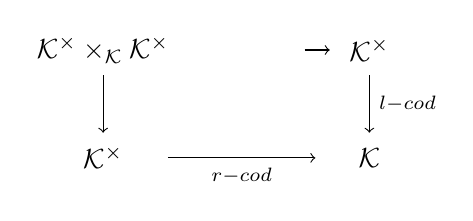
\begin{tikzpicture}[x=1.3em,y=1.3em]
  \node (a) at (0,1.5)   {$\mathcal{K}^{\times}\times_{\mathcal{K}}\mathcal{K}^{\times}$};
  \node (b) at (7.4,1.5) {$\mathcal{K}^{\times}$};
  \node (c) at (0,-1.5)  {$\mathcal{K}^{\times}$};
  \node (d) at (7.4,-1.5){$\mathcal{K}$};
  \draw[->] (5.6,1.5) -- (6.3,1.5);
  \draw[->] (0,0.8) -- (0,-0.8);
  \draw[->] (7.4,0.8) -- node[right]{$\scriptstyle\text{l-cod}$} (7.4,-0.8);
  \draw[->] (1.8,-1.5) -- node[below]{$\scriptstyle\text{r-cod}$} (5.9,-1.5);
  \node at (1.9,0.7) {$\scriptstyle\lrcorner$};
\end{tikzpicture}
\end{center}
是一个\trInfinityCosmos{}（见练习 6.1.iii），即水平可复合的一对双侧等价纤维化
$A\overset{q}{\twoheadleftarrow}E\overset{p}{\twoheadrightarrow}B\overset{r}{\twoheadleftarrow}F\overset{s}{\twoheadrightarrow}C$
之\trInfinityCosmos。复合\trFunctor{}
$\circ\colon\mathcal{K}^{\times}\times_{\mathcal{K}}\mathcal{K}^{\times}\to\mathcal{K}^{\times}$
把一对水平可复合的双侧等价纤维化送到一条选定的复合\trSpan，它仅在单纯自然同构的
意义下结合，这正是双侧等价纤维化的\trDoubleCategory{}中水平复合之「伪性」的
缘由。（非幺伪）双侧等价纤维化的\trDoubleCategory{}可以理解为这一结构的一个商：
把\trInfinityCosmos{} $\mathcal{K}$ 换成其底\trCategory，并把
$\mathrm{cod}\colon\mathcal{K}^{\times}\to\mathcal{K}\times\mathcal{K}$ 的诸纤维
换成诸商 1-范畴——后者拥有相同的对象，但其 hom-集被定义为切片\trFunctorSpace{}%
中诸顶点的\trIsomorphism{}类。

现在，任何\trCosmologicalFunctor{} $F\colon\mathcal{K}\to\mathcal{L}$ 都诱导诸%
\trCosmologicalFunctor
\begin{center}
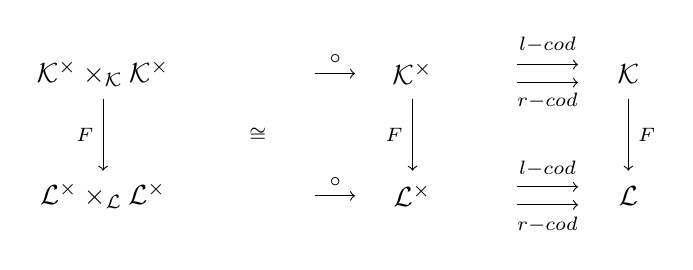
\begin{tikzpicture}[x=1.3em,y=1.3em]
  \node (a) at (0,1.7)    {$\mathcal{K}^{\times}\times_{\mathcal{K}}\mathcal{K}^{\times}$};
  \node (b) at (8.6,1.7)  {$\mathcal{K}^{\times}$};
  \node (c) at (14.6,1.7) {$\mathcal{K}$};
  \node (d) at (0,-1.7)   {$\mathcal{L}^{\times}\times_{\mathcal{L}}\mathcal{L}^{\times}$};
  \node (e) at (8.6,-1.7) {$\mathcal{L}^{\times}$};
  \node (f) at (14.6,-1.7){$\mathcal{L}$};
  \draw[->] (5.9,1.7) -- node[above]{$\scriptstyle\circ$} (7.0,1.7);
  \draw[->] (11.5,1.95) -- (13.2,1.95);
  \draw[->] (11.5,1.45) -- (13.2,1.45);
  \node at (12.35,2.5) {$\scriptstyle\text{l-cod}$};
  \node at (12.35,0.95) {$\scriptstyle\text{r-cod}$};
  \draw[->] (5.9,-1.7) -- node[above]{$\scriptstyle\circ$} (7.0,-1.7);
  \draw[->] (11.5,-1.45) -- (13.2,-1.45);
  \draw[->] (11.5,-1.95) -- (13.2,-1.95);
  \node at (12.35,-0.95) {$\scriptstyle\text{l-cod}$};
  \node at (12.35,-2.5) {$\scriptstyle\text{r-cod}$};
  \draw[->] (0,1.0) -- node[left]{$\scriptstyle F$} (0,-1.0);
  \draw[->] (8.6,1.0) -- node[left]{$\scriptstyle F$} (8.6,-1.0);
  \draw[->] (14.6,1.0) -- node[right]{$\scriptstyle F$} (14.6,-1.0);
  \node at (4.3,0) {$\scriptstyle\cong$};
\end{tikzpicture}
\end{center}
它们与诸余定义域\trFunctor{}严格交换，而与复合\trFunctor{}至多差一个同构。于是，
一个\trCosmologicalFunctor{}诱导双侧等价纤维化的诸\trDoubleCategory{}之间的一个
双函子，后者严格保持\trFunctor{}与方块的竖直复合，并在相干自然同构的意义下保持%
\trSpan{}与方块的水平复合。

由此得出：一个\trCosmologicalFunctor{}
$F\colon\mathcal{K}\to\mathcal{L}$ 诱导模的诸\trVirtualDoubleCategory{}之间的一个%
\trFunctor{} $F\colon\Mod(\mathcal{K})\to\Mod(\mathcal{L})$，它严格保持全部结构，
因为模映射的多范畴式复合派生自双侧等价纤维化的\trDoubleCategory{}中严格定义
的竖直复合。
\end{proof}

就其作为形式范畴论舞台的效用而言，至关重要的事实是：
模的\trVirtualDoubleCategory{}是一个\trVirtualEquipment，意谓它满足如下两条进
一步的性质：

\begin{enumerate}[label=(\roman*)]
\item 对任何一支\trModule{}与一对\trFunctor——如下左图所示——都存在一个%
\textbf{限制}\trModule{}与一支\textbf{笛卡尔的}\trCell，如下右图所示
\begin{center}
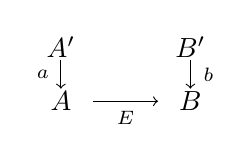
\begin{tikzpicture}[x=1.3em,y=1.3em]
  \node at (0,1.5) {$A'$};
  \node at (3.6,1.5) {$B'$};
  \node at (0,0) {$A$};
  \node at (3.6,0) {$B$};
  \draw[->] (0,1.15) -- (0,0.35);
  \node at (-0.5,0.75) {$\scriptstyle a$};
  \draw[->] (3.6,1.15) -- (3.6,0.35);
  \node at (4.1,0.75) {$\scriptstyle b$};
  \draw[->] (0.9,0) -- (2.7,0);
  \node at (1.8,-0.45) {$\scriptstyle E$};
\end{tikzpicture}
\qquad$\rightsquigarrow$\qquad
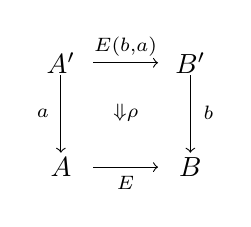
\begin{tikzpicture}[x=1.3em,y=1.3em]
  \node at (0,2.9) {$A'$};
  \node at (3.6,2.9) {$B'$};
  \node at (0,0) {$A$};
  \node at (3.6,0) {$B$};
  \draw[->] (0.9,2.9) -- (2.7,2.9);
  \node at (1.8,3.35) {$\scriptstyle E(b,a)$};
  \draw[->] (0,2.55) -- (0,0.4);
  \node at (-0.5,1.5) {$\scriptstyle a$};
  \draw[->] (3.6,2.55) -- (3.6,0.4);
  \node at (4.1,1.5) {$\scriptstyle b$};
  \node at (1.8,1.5) {$\scriptstyle\Downarrow\rho$};
  \draw[->] (0.9,0) -- (2.7,0);
  \node at (1.8,-0.45) {$\scriptstyle E$};
\end{tikzpicture}
\end{center}
并由如下\trUniversalProperty{}刻画：任何如下左图所示的\trCell{}都经由 $\rho$
唯一地分解，如下右图所示：
\begin{center}
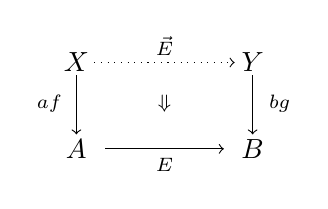
\begin{tikzpicture}[x=1.3em,y=1.3em]
  \node at (0,3) {$X$};
  \node at (4.9,3) {$Y$};
  \draw[->,dotted] (0.5,3) -- (4.4,3);
  \node at (2.45,3.45) {$\scriptstyle\vec{E}$};
  \draw[->] (0,2.65) -- (0,1.0);
  \node at (-0.75,1.85) {$\scriptstyle af$};
  \draw[->] (4.9,2.65) -- (4.9,1.0);
  \node at (5.65,1.85) {$\scriptstyle bg$};
  \node at (2.45,1.85) {$\scriptstyle\Downarrow$};
  \node at (0,0.6) {$A$};
  \node at (4.9,0.6) {$B$};
  \draw[->] (0.8,0.6) -- (4.1,0.6);
  \node at (2.45,0.15) {$\scriptstyle E$};
\end{tikzpicture}
\qquad $=$ \qquad
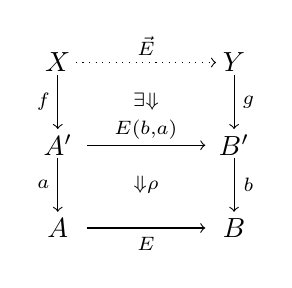
\begin{tikzpicture}[x=1.3em,y=1.3em]
  \node at (0,4.6) {$X$};
  \node at (4.9,4.6) {$Y$};
  \draw[->,dotted] (0.5,4.6) -- (4.4,4.6);
  \node at (2.45,5.05) {$\scriptstyle\vec{E}$};
  \draw[->] (0,4.25) -- (0,2.75);
  \node at (-0.4,3.5) {$\scriptstyle f$};
  \node at (2.45,3.5) {$\scriptstyle\exists\Downarrow$};
  \draw[->] (4.9,4.25) -- (4.9,2.75);
  \node at (5.3,3.5) {$\scriptstyle g$};
  \node at (0,2.3) {$A'$};
  \node at (4.9,2.3) {$B'$};
  \draw[->] (0.8,2.3) -- (4.1,2.3);
  \node at (2.45,2.72) {$\scriptstyle E(b,a)$};
  \draw[->] (0,1.95) -- (0,0.45);
  \node at (-0.4,1.2) {$\scriptstyle a$};
  \draw[->] (4.9,1.95) -- (4.9,0.45);
  \node at (5.3,1.2) {$\scriptstyle b$};
  \node at (2.45,1.2) {$\scriptstyle\Downarrow\rho$};
  \node at (0,0) {$A$};
  \node at (4.9,0) {$B$};
  \draw[->] (0.8,0) -- (4.1,0);
  \node at (2.45,-0.45) {$\scriptstyle E$};
\end{tikzpicture}
\end{center}
限制\trModule{}由把一支\trModule{} $A\xrightarrow{E}B$ 沿\trFunctor{}
$a\colon A'\to A$ 与 $b\colon B'\to B$ 作\trPullback{}而定义。定义
$E(b,a)$ 的那个单纯\trPullback{}诱导\trFunctorSpace{}之间的一个\trEquivalence
\begin{equation*}
\Fun_{af\times bg}(E_{1}\divideontimes\cdots\divideontimes E_{n},\,E)
\simeq
\Fun_{f\times g}(E_{1}\divideontimes\cdots\divideontimes E_{n},\,E(b,a)),
\end{equation*}
它给出这一\trUniversalProperty{}（见\cref{prop:restriction}）。
\item 每个对象 $A$ 都拥有一个\textbf{单位}\trModule，配备有一支零元\textbf{余笛卡尔的}%
\trCell
\begin{center}
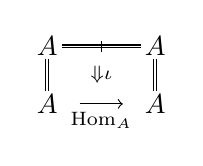
\begin{tikzpicture}[x=1.3em,y=1.3em]
  \node at (0,1.6) {$A$};
  \node at (3.0,1.6) {$A$};
  \node at (0,0) {$A$};
  \node at (3.0,0) {$A$};
  \draw[double,double distance=0.6pt] (0.4,1.6) -- (2.6,1.6);
  \draw (1.5,1.75) -- (1.5,1.45);
  \draw[double,double distance=0.6pt] (0,1.25) -- (0,0.35);
  \draw[double,double distance=0.6pt] (3.0,1.25) -- (3.0,0.35);
  \node at (1.5,0.8) {$\scriptstyle\Downarrow\iota$};
  \draw[->] (0.9,0) -- (2.1,0);
  \node at (1.5,-0.45) {$\scriptstyle\HomA$};
\end{tikzpicture}
\end{center}
满足如下\trUniversalProperty{}：模的\trVirtualDoubleCategory{}中任何水平源包含
对象 $A$ 的\trCell——如下左图所示——都经由 $\iota$ 唯一地分解，如下右图所示：
\begin{center}
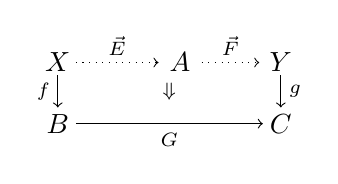
\begin{tikzpicture}[x=1.3em,y=1.3em]
  \node at (0,1.7) {$X$};
  \node at (3.4,1.7) {$A$};
  \node at (6.2,1.7) {$Y$};
  \draw[->,dotted] (0.5,1.7) -- (2.8,1.7);
  \node at (1.65,2.15) {$\scriptstyle\vec{E}$};
  \draw[->,dotted] (4.0,1.7) -- (5.6,1.7);
  \node at (4.8,2.15) {$\scriptstyle\vec{F}$};
  \draw[->] (0,1.35) -- (0,0.45);
  \node at (-0.4,0.9) {$\scriptstyle f$};
  \draw[->] (6.2,1.35) -- (6.2,0.45);
  \node at (6.6,0.9) {$\scriptstyle g$};
  \node at (3.1,0.9) {$\scriptstyle\Downarrow$};
  \node at (0,0) {$B$};
  \node at (6.2,0) {$C$};
  \draw[->] (0.5,0) -- (5.7,0);
  \node at (3.1,-0.45) {$\scriptstyle G$};
\end{tikzpicture}
\qquad $=$ \qquad
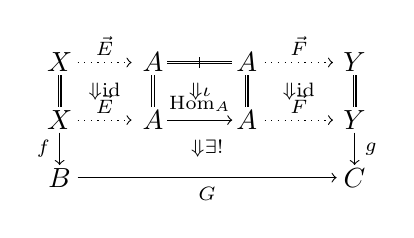
\begin{tikzpicture}[x=1.3em,y=1.3em]
  \node at (0,3.4) {$X$};
  \node at (2.6,3.4) {$A$};
  \node at (5.2,3.4) {$A$};
  \node at (8.2,3.4) {$Y$};
  \draw[->,dotted] (0.5,3.4) -- (2.0,3.4);
  \node at (1.25,3.85) {$\scriptstyle\vec{E}$};
  \draw[double,double distance=0.6pt] (3.0,3.4) -- (4.8,3.4);
  \draw (3.9,3.55) -- (3.9,3.25);
  \draw[->,dotted] (5.7,3.4) -- (7.6,3.4);
  \node at (6.65,3.85) {$\scriptstyle\vec{F}$};
  \draw[double,double distance=0.6pt] (0,3.05) -- (0,2.15);
  \draw[double,double distance=0.6pt] (2.6,3.05) -- (2.6,2.15);
  \draw[double,double distance=0.6pt] (5.2,3.05) -- (5.2,2.15);
  \draw[double,double distance=0.6pt] (8.2,3.05) -- (8.2,2.15);
  \node at (1.25,2.6) {$\scriptstyle\Downarrow\mathrm{id}$};
  \node at (3.9,2.6) {$\scriptstyle\Downarrow\iota$};
  \node at (6.65,2.6) {$\scriptstyle\Downarrow\mathrm{id}$};
  \node at (0,1.8) {$X$};
  \node at (2.6,1.8) {$A$};
  \node at (5.2,1.8) {$A$};
  \node at (8.2,1.8) {$Y$};
  \draw[->,dotted] (0.5,1.8) -- (2.0,1.8);
  \node at (1.25,2.25) {$\scriptstyle\vec{E}$};
  \draw[->] (3.0,1.8) -- (4.8,1.8);
  \node at (3.9,2.25) {$\scriptstyle\HomA$};
  \draw[->,dotted] (5.7,1.8) -- (7.6,1.8);
  \node at (6.65,2.25) {$\scriptstyle\vec{F}$};
  \draw[->] (0,1.45) -- (0,0.55);
  \node at (-0.45,1.0) {$\scriptstyle f$};
  \draw[->] (8.2,1.45) -- (8.2,0.55);
  \node at (8.65,1.0) {$\scriptstyle g$};
  \node at (4.1,1.0) {$\scriptstyle\Downarrow\exists!$};
  \node at (0,0.2) {$B$};
  \node at (8.2,0.2) {$C$};
  \draw[->] (0.5,0.2) -- (7.7,0.2);
  \node at (4.1,-0.25) {$\scriptstyle G$};
\end{tikzpicture}
\end{center}
单位\trModule{}即箭头∞-范畴，当把它视为一个从 $A$ 到 $A$ 的\trModule{}时，记作
$A\xrightarrow{\HomA}A$。这一\trUniversalProperty{}由\trYonedaLemma{}得出（见
\cref{prop:units}）。
\end{enumerate}

\cref{lem:cosmological-functor-induces-vdc-functor}扩张到诸模的虚拟装备：

\begin{proposition}\label{prop:cosmological-functor-induces-ve-functor}
一个\trCosmologicalFunctor{}
$F\colon\mathcal{K}\to\mathcal{L}$ 诱导诸\trVirtualEquipment{}之间的%
\trFunctor{}
$F\colon\Mod(\mathcal{K})\to\Mod(\mathcal{L})$，并保持全部结构。
\end{proposition}

\begin{proof}
鉴于\cref{lem:cosmological-functor-induces-vdc-functor}，尚需考虑的只是单位与
限制的\trModule{}及\trCell。由\cref{prop:units}与\cref{prop:restriction}的证明中
所给的构造，立见这些皆为诸\trCosmologicalFunctor{}所保持：
\begin{center}
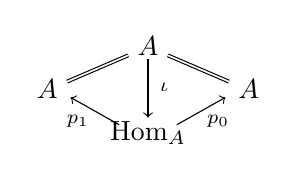
\begin{tikzpicture}[x=1.3em,y=1.3em]
  \node at (0,2.4) {$A$};
  \node at (-2.8,1.2) {$A$};
  \node at (2.8,1.2) {$A$};
  \node at (0,0) {$\HomA$};
  \draw[double,double distance=0.6pt] (-0.55,2.15) -- (-2.25,1.42);
  \draw[double,double distance=0.6pt] (0.55,2.15) -- (2.25,1.42);
  \draw[->] (0,2.05) -- (0,0.42);
  \node at (0.45,1.25) {$\scriptstyle\iota$};
  \draw[->] (-0.8,0.22) -- (-2.15,0.98);
  \node at (-1.95,0.32) {$\scriptstyle p_{1}$};
  \draw[->] (0.8,0.22) -- (2.15,0.98);
  \node at (1.95,0.32) {$\scriptstyle p_{0}$};
\end{tikzpicture}
\qquad
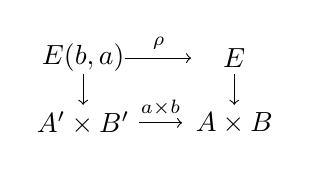
\begin{tikzpicture}[x=1.3em,y=1.3em]
  \node at (0,1.8) {$E(b,a)$};
  \node at (4.2,1.8) {$E$};
  \node at (0,0) {$A'\times B'$};
  \node at (4.2,0) {$A\times B$};
  \draw[->] (1.15,1.8) -- (3.0,1.8);
  \node at (2.1,2.22) {$\scriptstyle\rho$};
  \draw[->] (0,1.35) -- (0,0.5);
  \draw[->] (4.2,1.35) -- (4.2,0.5);
  \draw[->] (1.55,0) -- (2.75,0);
  \node at (2.15,0.42) {$\scriptstyle a\times b$};
  \node at (3.55,1.3) {$\scriptstyle\lrcorner$};
\end{tikzpicture}
\end{center}
\end{proof}

\trHomotopyTwoCategory{} $\mathfrak{h}\mathcal{K}$ 中的诸\trFunctor{}与诸%
\trNaturalTransformation{}以三种方式嵌入虚拟装备 $\Mod(\mathcal{K})$ 之中。一个%
\trFunctor{} $f\colon A\to B$ 既被表示为一支竖直箭头，也被表示为那对水平的%
\trModule{} $A\xrightarrow{\HomB(B,f)}B$ 与
$B\xrightarrow{\HomB(f,B)}A$，它们以一种适宜于\trVirtualDoubleCategory{}的意义
表现得如同伴随：\trModule{} $A\xrightarrow{\HomB(B,f)}B$ 定义竖直箭头
$f\colon A\to B$ 的一个\emph{\trCompanion}，而\trModule{}
$B\xrightarrow{\HomB(f,B)}A$ 则定义其一个\emph{\trConjoint}（见
\cref{prop:representable-restriction-application}、\cref{thm:spider-lemma}与
\cref{cor:represented-composites}）。借助\cref{prop:two-cell-bijections}，这些
嵌入扩张到诸\trNaturalTransformation{}上：对任何平行的\trFunctor{}对，在同伦
2-范畴
\begin{center}
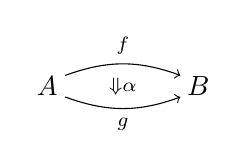
\begin{tikzpicture}[x=1.3em,y=1.3em]
  \node (a) at (0,0) {$A$};
  \node (b) at (4.2,0) {$B$};
  \draw[->] (0.5,0.3) to[bend left=20] node[above,pos=0.5]{$\scriptstyle f$} (3.7,0.3);
  \draw[->] (0.5,-0.3) to[bend right=20] node[below,pos=0.5]{$\scriptstyle g$} (3.7,-0.3);
  \node at (2.1,0) {$\scriptstyle\Downarrow\alpha$};
\end{tikzpicture}
\end{center}
中的诸\trNaturalTransformation{}与模的\trVirtualEquipment{}中的诸\trCell{}之间
存在自然双射：
\begin{center}
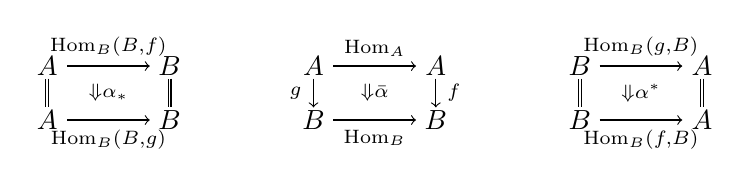
\begin{tikzpicture}[x=1.3em,y=1.3em]
  \node at (0,1.5) {$A$};
  \node at (3.4,1.5) {$B$};
  \node at (0,0) {$A$};
  \node at (3.4,0) {$B$};
  \draw[->] (0.55,1.5) -- node[above]{$\scriptstyle\HomB(B,f)$} (2.85,1.5);
  \draw[->] (0.55,0) -- node[below]{$\scriptstyle\HomB(B,g)$} (2.85,0);
  \draw[double,double distance=0.6pt] (0,1.15) -- (0,0.35);
  \draw[double,double distance=0.6pt] (3.4,1.15) -- (3.4,0.35);
  \node at (1.7,0.75) {$\scriptstyle\Downarrow\alpha_{*}$};
  \node at (5.4,0.75) {$\scriptstyle\rightsquigarrow$};
  \begin{scope}[shift={(7.4,0)}]
  \node at (0,1.5) {$A$};
  \node at (3.4,1.5) {$A$};
  \node at (0,0) {$B$};
  \node at (3.4,0) {$B$};
  \draw[->] (0.55,1.5) -- node[above]{$\scriptstyle\HomA$} (2.85,1.5);
  \draw[->] (0.55,0) -- node[below]{$\scriptstyle\HomB$} (2.85,0);
  \draw[->] (0,1.15) -- (0,0.35);
  \node at (-0.5,0.75) {$\scriptstyle g$};
  \draw[->] (3.4,1.15) -- (3.4,0.35);
  \node at (3.9,0.75) {$\scriptstyle f$};
  \node at (1.7,0.75) {$\scriptstyle\Downarrow\bar{\alpha}$};
  \end{scope}
  \node at (12.8,0.75) {$\scriptstyle\rightsquigarrow$};
  \begin{scope}[shift={(14.8,0)}]
  \node at (0,1.5) {$B$};
  \node at (3.4,1.5) {$A$};
  \node at (0,0) {$B$};
  \node at (3.4,0) {$A$};
  \draw[->] (0.55,1.5) -- node[above]{$\scriptstyle\HomB(g,B)$} (2.85,1.5);
  \draw[->] (0.55,0) -- node[below]{$\scriptstyle\HomB(f,B)$} (2.85,0);
  \draw[double,double distance=0.6pt] (0,1.15) -- (0,0.35);
  \draw[double,double distance=0.6pt] (3.4,1.15) -- (3.4,0.35);
  \node at (1.7,0.75) {$\scriptstyle\Downarrow\alpha^{*}$};
  \end{scope}
\end{tikzpicture}
\end{center}

正如\cref{def:covariant-contravariant-embeddings}中所评述的，作为这些结果的一
个推论，存在三个从\trHomotopyTwoCategory{} $\mathfrak{h}\mathcal{K}$ 到虚拟装备
$\Mod(\mathcal{K})$ 的\trLocallyFullyFaithful\trHomomorphism。命题 8.3.18 所描述的那个%
\emph{竖直嵌入}（vertical embedding）把 $\mathfrak{h}\mathcal{K}$ 的诸\trFunctor{}%
送到竖直箭头，并把诸 2-\trCell{}送到源与靶由单位\trModule{}给出的一元\trCell。
另外两个分别是\emph{协变嵌入}与\emph{逆变嵌入}——它们把同伦 2-范畴嵌入到
$\Mod(\mathcal{K})$ 的那个仅由竖直边界皆为恒同的一元\trCell{}构成的子结构%
\footnote{这一子结构十分接近一个\trBicategory，其中一元\trCell{}的水平复合如定义
8.3.16 那样构造，只是诸\trModule{}的相容序列并不总是拥有一个水平复合。}之中。
协变嵌入像中的诸\trModule{}是诸右可表示模，而逆变嵌入像中的诸\trModule{}则是诸
左可表示模。我们把它留给读者验证：

\begin{lemma}\label{lem:vdc-functor-commutes-with-embeddings}
由一个\trCosmologicalFunctor{}
$F\colon\mathcal{K}\to\mathcal{L}$ 所诱导的诸\trVirtualEquipment{}之间的%
\trFunctor{}
$F\colon\Mod(\mathcal{K})\to\Mod(\mathcal{L})$ 与协变嵌入、逆变嵌入及竖直嵌入相
交换。
\end{lemma}

\begin{proof}
\cref{ex:prove-embeddings-commute}。
\end{proof}

第 9 章的主题可以这样概括：一个\trInfinityCosmos{}中的模的\trVirtualEquipment{}%
是发展诸\trInfinityCategory{}的范畴论的一个稳健舞台。一方面，它包含该%
\trInfinityCosmos{}的\trHomotopyTwoCategory——第一部分中的大多数结果正是以此为
舞台的。它也是研究那些在\trHomotopyTwoCategory{}中颇为难于表述的∞-范畴性质的
一个十分自然的家园。例如，逗号∞-范畴的弱 2-泛性质现在由\cref{lem:comma-module-maps-bijection}
中的一个双射所编码：虚拟装备中余定义域为\trCommaModule{}的诸\trCell{}，与%
\trHomotopyTwoCategory{}中特定形状的诸\trNaturalTransformation{}一一对应。
\trModule{}的\trFiberedEquivalence——第 4 章中曾用它们来表达\trAdjunction、%
\trLimit{}与\trColimit{}的诸\trUniversalProperty——现在是虚拟装备中平行的%
\trModule{}之间的竖直\trIsomorphism。该虚拟装备还干净利落地编码了逐点左%
\trKanExtension{}与右\trKanExtension{}的\trUniversalProperty，这些%
\trKanExtension{}正是用来定义
诸\trInfinityCategory{}之间的\trFunctor{}的（加权）\trLimit{}与\trColimit{}的
概念。

我们将证明：当 $F\colon\mathcal{K}\Rightarrow\mathcal{L}$ 是一个%
\trCosmologicalBiequivalence{}时，相应的诸虚拟装备之间的\trFunctor{}是某种适宜
意义下的一个\trBiequivalence。为追求这一结果，我们首先对命题 10.3.1(xiii) 加以
细化。

\begin{proposition}\label{prop:biequivalence-preserves-modules}
一个\trCosmologicalBiequivalence{}
$F\colon\mathcal{K}\Rightarrow\mathcal{L}$ 保持、反射并创造诸\trModule：
\begin{enumerate}[label=(\roman*)]
\item 一支\trIsofibration{} $(q,p)\colon E\twoheadrightarrow A\times B$ 是
$\mathcal{K}$ 中的\trModule，当且仅当
$(Fq,Fp)\colon FE\twoheadrightarrow FA\times FB$ 是 $\mathcal{L}$ 中的%
\trModule。
\item 一对\trModule{} $A\xrightarrow{E}B$ 与 $A\xrightarrow{E'}B$ 在
$\mathcal{K}$ 中\trEquivalence，当且仅当诸\trModule{}
$FA\xrightarrow{FE}FB$ 与 $FA\xrightarrow{FE'}FB$ 在 $\mathcal{L}$ 中定义
等价的\trModule。
\item 对 $\mathcal{L}$ 中的每一个\trModule{} $A'\xrightarrow{G}B'$ 以及
$\mathcal{K}$ 中的每一对带有指定\trEquivalence{} $FA\simeq A'$ 与
$FB\simeq B'$ 的\trInfinityCategory{} $A$、$B$，存在 $\mathcal{K}$ 中的一个%
\trModule{} $A\xrightarrow{E}B$，使得 $FE$ 在这对\trEquivalence{}之上等价于
$G$。
\end{enumerate}
\end{proposition}

\begin{proof}
(i) 的结果已在命题 10.3.1(xiii) 中证明。
(ii) 的结果从如下事实得出：受诱导的\trCosmologicalBiequivalence
\begin{center}
\begin{tikzpicture}[x=1.05em,y=1.05em]
  \node (a) at (0,1.7)    {${}_{A}\Mod(\mathcal{K})_{/B}$};
  \node (b) at (12.0,1.7) {${}_{FA}\Mod(\mathcal{L})_{/FB}$};
  \node (c) at (0,-1.7)   {$\mathcal{K}_{/A\times B}$};
  \node (d) at (12.8,-1.7){$\mathcal{L}_{/FA\times FB}$};
  \draw[->,dashed] (4.0,1.7) -- node[above=9pt]{$\scriptstyle F$} node[above=1pt]{$\scriptstyle\sim$} (8.0,1.7);
  \draw[->] (2.2,-1.7) -- node[above]{$\scriptstyle F$} node[below]{$\scriptstyle\sim$} (9.6,-1.7);
  \draw[right hook->] (0,1.0) -- (0,-1.0);
  \draw[right hook->] (12.4,1.0) -- (12.4,-1.0);
\end{tikzpicture}
\end{center}
保持并反射对象之间的诸\trEquivalence。

就 (iii) 而言，固定一对\trEquivalence{} $FA\simeq A'$ 与 $FB\simeq B'$，它们
定义一支\trEquivalence{} $e\colon A'\times B'\simeq FA\times FB$，并考虑复合%
\trBiequivalence
\begin{equation*}
\mathcal{K}_{/A\times B}
\xrightarrow[\ \sim\ ]{\ F\ }
\mathcal{L}_{/FA\times FB}
\xrightarrow[\ \sim\ ]{\ e^{*}\ }
\mathcal{L}_{/A'\times B'}
\end{equation*}
它由第 10 章中的\cref{prop:slice-biequivalence}与\cref{prop:pullback-biequivalence}给出。考虑一个\trModule{}
$G\twoheadrightarrow A'\times B'$。由本质满性，存在一支\trIsofibration{}
$E\twoheadrightarrow A\times B$，其在这个\trCosmologicalFunctor{}之下的像——
即 $FE\twoheadrightarrow FA\times FB$ 沿
$e\colon A'\times B'\simeq FA\times FB$ 的\trPullback——定义一支%
\trIsofibration{} $(q,p)\colon E'\twoheadrightarrow A'\times B'$，后者在
$\mathcal{L}_{/A'\times B'}$ 中等价于 $G$。余下的只是论证：$E$ 定义一个从 $A$
到 $B$ 的\trModule；这一点将本质上如 (i) 的证明那样，从「$E'\simeq G$ 定义一
个从 $A'$ 到 $B'$ 的\trModule」这一事实得出。

由于 $E$ 的像 $E'$ 等价于一个\trDiscrete{}对象，命题 10.3.6(v) 告诉我们：$E$
在 $\mathcal{K}_{/A\times B}$ 中是\trDiscrete{}。

最后一步是论证：所需要的 $E\to\HomB(B,p)$ 的那个\trRightAdjoint{}存在于%
\trBiequivalence{}
$\mathcal{K}_{/A\times B}\Rightarrow\mathcal{L}_{/A'\times B'}$ 的像之中，再应
用命题 10.3.6(iii) 推断其在 $\mathcal{K}_{/A\times B}$ 中的存在性；一个类似的
论证当然也适用于\trFunctor{} $E\to\HomA(q,A)$。为见此，注意
$F\colon\mathcal{K}_{/A\times B}\Rightarrow\mathcal{L}_{/FA\times FB}$ 把
$\HomB(B,p)\twoheadrightarrow A\times B$ 送到
$\Hom_{FB}(FB,Fp)\twoheadrightarrow FA\times FB$。由 (i)，只需论证这个\trFunctor{}%
在 $FA\times FB$ 之上有一个\trRightAdjoint。把命题 10.3.6(iii) 应用于%
\trBiequivalence{}
$e^{*}\colon\mathcal{L}_{/FA\times FB}\Rightarrow\mathcal{L}_{/A'\times B'}$，
这便从「$E'\to\Hom_{B'}(B',p')$ 在 $A'\times B'$ 之上有一个\trRightAdjoint」
这一事实得出。
\end{proof}

\begin{proposition}\label{prop:right-representability-invariance}
设 $F\colon\mathcal{K}\Rightarrow\mathcal{L}$ 是一个\trCosmologicalBiequivalence。
那么 $\mathcal{K}$ 中的一个\trModule{} $A\xrightarrow{E}B$ 是右可表示的，当且
仅当\trModule{} $FA\xrightarrow{FE}FB$ 在 $\mathcal{L}$ 中是右可表示的；在此情
形下，$F$ 把 $\mathcal{K}$ 中的表示\trFunctor{} $f\colon A\to B$ 送到
$\mathcal{L}$ 中的表示\trFunctor{} $Ff\colon FA\to FB$。
\end{proposition}

\begin{proof}
说 $\mathcal{K}$ 中的\trModule{} $A\xrightarrow{E}B$ 是右可表示的，即是说存在
一个\trFunctor{} $f\colon A\to B$ 连同诸\trModule{}在 $B$ 之上的一个%
\trEquivalence{} $E\simeq_{A\times B}\HomB(B,f)$。若是如此，则任何%
\trCosmologicalFunctor{}
$F\colon\mathcal{K}\to\mathcal{L}$ 都把它送到一支\trFiberedEquivalence{}
$FE\simeq_{FA\times FB}\Hom_{FB}(FB,Ff)$，从而\trModule{}
$FA\xrightarrow{FE}FB$ 在 $\mathcal{L}$ 中被 $Ff\colon FA\to FB$ 右表示。

反过来，若 $FA\xrightarrow{FE}FB$ 被某个\trFunctor{} $g\colon FA\to FB$ 右表
示，则由推论 10.3.2(ii)，存在 $\mathcal{K}$ 中的一个\trFunctor{}
$f\colon A\to B$ 使得在 $\mathcal{L}$ 中 $Ff\simeq g$。由
\cref{prop:two-cell-bijections}，自然同构的\trFunctor{}表示等价的\trModule；即
$\Hom_{FB}(FB,g)\simeq_{FA\times FB}\Hom_{FB}(FB,Ff)$。于是
$FE\simeq_{FA\times FB}\Hom_{FB}(FB,Ff)$。由
\cref{prop:biequivalence-preserves-modules}(ii)，这支\trFiberedEquivalence{}沿%
\trCosmologicalFunctor{}
$F\colon\mathcal{K}_{/A\times B}\to\mathcal{L}_{/FA\times FB}$ 提升为一支%
\trFiberedEquivalence{} $E\simeq_{A\times B}\HomB(B,f)$，这就证明 $E$ 在
$\mathcal{K}$ 中被 $f\colon A\to B$ 右表示。
\end{proof}

我们已经看到，诸\trCosmologicalFunctor{}诱导诸虚拟装备之间的\trFunctor，保持
全部结构。当一个\trCosmologicalFunctor{}是一个\trBiequivalence{}时，受诱导的
诸虚拟装备之间的\trFunctor{}还创造结构并反射诸\trUniversalProperty，其依据是我
们现在即将逐一列出的这批双射。

\begin{theorem}[\trInfinityCategory{}论的\trModelIndependence]\label{thm:biequivalence-of-virtual-equipments}
若 $F\colon\mathcal{K}\Rightarrow\mathcal{L}$ 是一个\trCosmologicalBiequivalence，
则受诱导的诸虚拟装备之间的\trFunctor
\begin{equation*}
F\colon \Mod(\mathcal{K})\Rightarrow\Mod(\mathcal{L})
\end{equation*}
定义\textbf{诸虚拟装备之间的一个\trBiequivalence}：亦即，它
\begin{enumerate}[label=(\roman*)]
\item 在对象的\trEquivalence{}类上为双射；
\item 在平行的竖直\trFunctor{}的同构类上为局部双射，并扩充 (i) 的双射；
\item 在平行的\trModule{}的\trEquivalence{}类上为局部双射，并扩充 (ii) 的双射；
\item 在诸\trCell{}上为局部双射，并扩充 (i)、(ii) 与 (iii) 的双射。
\end{enumerate}
\end{theorem}

还需进一步注意：若两个\trInfinityCosmos{}由一条由有限多支\trBiequivalence{}构
成的之字形链相连，则\cref{thm:biequivalence-of-virtual-equipments}所描述的诸
双射可以复合。

\begin{proof}
性质 (i) 与 (ii) 是推论 10.3.2(i) 与 (ii) 的复述。
局部双射 (iii) 立即从\cref{prop:biequivalence-preserves-modules}以及如下事实得
出：对任何一对\trEquivalence{}
$e\colon A'\times B'\simeq FA\times FB$，复合\trBiequivalence
\begin{equation*}
\mathcal{K}_{/A\times B}
\xrightarrow[\ \sim\ ]{\ F\ }
\mathcal{L}_{/FA\times FB}
\xrightarrow[\ \sim\ ]{\ e^{*}\ }
\mathcal{L}_{/A'\times B'}
\end{equation*}
保持、反射并创造对象之间的诸\trEquivalence——这再次由推论 10.3.2(i) 得出。最
后，(iv) 是推论 10.3.2(ii) 在这个\trCosmologicalBiequivalence{}上的一个应用。
\end{proof}

\cref{thm:biequivalence-of-virtual-equipments}涵盖了迄今确立的许多%
\trModelIndependence{}陈述。例如，诸\trInfinityCategory{}之间的\trAdjunction{}%
之存在与一个\trInfinityCategory{}内部的\trLimit{}与\trColimit{}之存在，都可以
被编码为模的\trVirtualEquipment{}中一条\trEquivalence{}不变的命题。逐点右%
\trExtension{}与左\trExtension{}的\trModelIndependence——最先在命题 10.3.8 中
证明——也可以作为\cref{thm:biequivalence-of-virtual-equipments}的一个初等推论
而确立，论证留给\cref{ex:pointwise-extensions-via-modules}。沿着同样的思路，诸
虚拟装备之间的一个\trBiequivalence{}保持、反射并创造诸\trModule{}的复合：

\begin{lemma}\label{lem:biequivalence-and-composites}
设 $F\colon\mathcal{K}\Rightarrow\mathcal{L}$ 是一个\trCosmologicalBiequivalence。
\begin{enumerate}[label=(\roman*)]
\item 那么，$\mathcal{K}$ 中模的一个相容序列在 $\Mod(\mathcal{K})$ 中拥有一个
复合，当且仅当该序列的像在 $\Mod(\mathcal{L})$ 中拥有一个复合。
\item 因此，诸\trCosmologicalBiequivalence{}保持并反射\trExactSquare。
\end{enumerate}
\end{lemma}

\begin{proof}
经由\cref{def:exact-square}，(ii) 立即从 (i) 得出，故尚需证明的只是：诸虚拟装备
之间的一个\trBiequivalence{}
$F\colon\Mod(\mathcal{K})\Rightarrow\Mod(\mathcal{L})$ 保持、反射并创造诸%
\trModule{}的复合。为见一支 $n$ 元复合\trCell{}
$\mu\colon E_{1}\divideontimes\cdots\divideontimes E_{n}\Rightarrow E$
被保持\footnote{原书于此处及下文「module
$A_{0}\xrightarrow{E}A_{n}$」处均印作「in $\mathfrak{h}\mathcal{K}$」。按文义，
$n$ 元复合胞与模均居于模的虚拟装备 $\Mod(\mathcal{K})$ 之中，而非同伦
2-范畴（对照引理 11.1.7(i) 自身「modules in $\mathcal{K}$ … a composite in
$\Mod(\mathcal{K})$」之措辞），疑为排印之误，两处均径改。——译者注}，注意由
\cref{thm:biequivalence-of-virtual-equipments}(iv)，$\Mod(\mathcal{L})$ 中的任
何\trCell{}都同构于 $F$ 的像中的一支\trCell：首先把诸对象替换为像中与之等价
者，然后把诸竖直\trFunctor{}替换为像中与之自然同构者，随后沿其∞-范畴性源与靶
之间指定的诸\trEquivalence{}把诸\trModule{}替换为像中与之等价者，最后应用局部
双射 (iv)，经由与这批数据作复合，把 $\Mod(\mathcal{L})$ 中的这个\trCell{}替换
为 $\Mod(\mathcal{K})$ 的像中唯一的一支\trCell。现在，由局部全忠实性与本质满
性，余笛卡尔的\trCell{}
$\mu\colon E_{1}\divideontimes\cdots\divideontimes E_{n}\Rightarrow E$ 的%
\trUniversalProperty{}蕴含：其像
$F\mu\colon FE_{1}\divideontimes\cdots\divideontimes FE_{n}\Rightarrow FE$
仍是一支余笛卡尔的\trCell。如此，复合
$E_{1}\otimes\cdots\otimes E_{n}\simeq E$ 为诸\trCosmologicalBiequivalence{}所
保持。

现在，若
$F\mu\colon FE_{1}\divideontimes\cdots\divideontimes FE_{n}\Rightarrow FE$
是一个复合，则由于 $F\colon\Mod(\mathcal{K})\to\Mod(\mathcal{L})$ 是%
\trLocallyFullyFaithful{}，
$\mu\colon E_{1}\divideontimes\cdots\divideontimes E_{n}\Rightarrow E$ 也是一
个复合；如此，复合
$FE_{1}\otimes\cdots\otimes FE_{n}\simeq FE$ 为诸\trCosmologicalBiequivalence{}%
所反射。

最后，假设 $\Mod(\mathcal{L})$ 中诸\trModule{}的序列
$FE_{1}\divideontimes\cdots\divideontimes FE_{n}$ 拥有一个复合
$FA_{0}\xrightarrow{G}FA_{n}$；由于\trModule{}的这个相容序列位于 $F$ 的像之
中，复合\trModule{} $G$ 的源与靶∞-范畴亦然。由
\cref{thm:biequivalence-of-virtual-equipments}(iii)，存在一个\trModule{}
$A_{0}\xrightarrow{E}A_{n}$，使得 $FE\simeq G$（作为从 $FA_{0}$ 到 $FA_{n}$
的\trModule）。见证这一复合关系的那支余笛卡尔的\trCell{}
$FE_{1}\divideontimes\cdots\divideontimes FE_{n}\Rightarrow G$ 与这支%
\trEquivalence{}的一元\trCell{}复合，从而定义一支余笛卡尔的\trCell{}
$FE_{1}\divideontimes\cdots\divideontimes FE_{n}\Rightarrow FE$。由
\cref{thm:biequivalence-of-virtual-equipments}(iv)，它提升为 $\Mod(\mathcal{K})$
中的一支 $n$ 元\trCell{}
$E_{1}\divideontimes\cdots\divideontimes E_{n}\Rightarrow E$。正如我们刚刚所见，
诸\trCell{}的余笛卡尔性为诸\trBiequivalence{}
$F\colon\Mod(\mathcal{K})\Rightarrow\Mod(\mathcal{L})$ 所反射，这就完成了「复
合为诸\trCosmologicalBiequivalence{}所创造」的证明。
\end{proof}

\cref{thm:biequivalence-of-virtual-equipments}的要点——亦即我们把它视为∞-范
畴论的\trModelIndependence{}之一个证明的理由——在于：任何关于诸%
\trInfinityCategory{}的、能够被编码进「虚拟装备的语言」之中的陈述，在%
\trChangeOfModel{}之下不变。我们的经验给了我们对这一语言的某种非正式理解。它
包括那些把一个\trInfinityCategory{}刻画到\trEquivalence{}（例如一个%
\trCommaInfinityCategory{}或一个\trArrowInfinityCategory）、或把一个\trFunctor{}%
刻画到自然同构（例如一个左或右伴随）的陈述。其他的\trModelIndependent{}陈述则是那些可以表
达为诸\trModule{}之间的一个\trEquivalence{}（例如关于诸\trModule{}的左或右可
表示性的结果）、或以具有某些性质的诸\trModule{}之间的一支\trCell{}之存在性来
表达的陈述（例如逐点\trExtension{}的情形）。但是，正如我们将发现的，通过利用
一种我们现在即将引入的逻辑框架，这种\trModelIndependent{}语言可以得到远为形式化的描述。

\subsection*{练习}

\begin{exercise}\label{ex:adhoc-model-independence}
请任选一个你最喜爱的\trInfinityCategory{}性概念，并给出其\trModelIndependence{}%
的一个特设证明。请将此与利用\cref{thm:biequivalence-of-virtual-equipments}的一
个证明相比较。
\end{exercise}

\begin{exercise}\label{ex:prove-embeddings-commute}
证明\cref{lem:vdc-functor-commutes-with-embeddings}。
\end{exercise}

\begin{exercise}\label{ex:pointwise-extensions-via-modules}
请利用\cref{thm:biequivalence-of-virtual-equipments}给出一个模论式的证明，以证
诸\trCosmologicalBiequivalence{}保持、反射并创造逐点右\trExtension{}与左%
\trExtension，并将这一论证与命题 10.3.8 的证明相比较。
\end{exercise}

\begin{exercise}\label{ex:initial-final-functors}
请证明：诸\trCartesianClosed{}\trInfinityCosmos{}之间的诸%
\trCosmologicalBiequivalence{}保持并反射初始\trFunctor{}与最终\trFunctor。
\end{exercise}

   %
\providecommand{\Fun}{\operatorname{Fun}}
\providecommand{\QCat}{\mathcal{Q}\mathcal{C}at}
\providecommand{\CSS}{\mathcal{C}\mathcal{S}\mathcal{S}}
\providecommand{\Set}{\mathcal{S}et}
\providecommand{\Cat}{\mathcal{C}at}
\providecommand{\hciso}{\mathbb{I}}  %

\section{带依赖排序的一阶逻辑}\label{sec:first-order-logic-dependent-sorts}

\trInfinityCategory{}论在\trChangeOfModel{}之下的不变性有一项重要的告诫。在从一个%
\trCompleteSegalSpaces{}过渡到其\trUnderlyingQuasiCategory{}再折返之后
\begin{equation*}
\CSS\ \xrightarrow[\ \sim\ ]{\ (-)_{0}\ }\ \QCat\ \xrightarrow[\ \sim\ ]{\ \mathrm{nerve}\ }\ \CSS
\end{equation*}
所得的\trCompleteSegalSpaces{}与原来那个等价，但多半不与之相等。但即便在经典的
严格情形，也并非关于 1-\trCategory{}的每一个陈述都在\trEquivalence{}之下不变：
「此\trCategory{}只有一个对象」就是一个著名的反例。类似地，并非关于 2-\trCategory{}的
每一个陈述都在\trBiequivalence{}之下不变。例如，考虑\cref{prop:cartesian-closure}为诸%
\trHomotopyTwoCategory{}所证明的那个陈述：「此 2-\trCategory{}有一个%
\trTwoTerminalObject」。设 $F\colon\mathcal{C}\Rightarrow\mathcal{D}$ 是 2-\trCategory{}之间的一个%
\trBiequivalence，而 $\mathcal{D}$ 有一个\trTwoTerminalObject{} $t$，那么由本质满性，
存在一个 $s\in\mathcal{C}$ 使得在 $\mathcal{D}$ 中 $Fs\simeq t$。但\trLocalEquivalence{}性质
只提供一支\trEquivalence
\begin{equation*}
\mathcal{C}(c,s)\simeq\mathcal{D}(Fc,Fs)\simeq\mathcal{D}(Fc,t)\cong 1,
\end{equation*}
它使 $s$ 成为一个\emph{双终对象}（biterminal object），却未必是一个%
\trTwoTerminalObject。

模型无关性定理（\cref{thm:biequivalence-of-virtual-equipments}）为由任何一对双等
价的\trInfinityCosmos{}所定义的模的%
\trVirtualEquipment{}提供一个\trBiequivalence。
由于关于\trInfinityCategories{}的重要陈述都可以表述为\trVirtualEquipment{}的性质，
这个\trBiequivalence{}便给出一种机制，使得用∞-\trCategory{}的某一个模型证明的
结果得以借之转移到另一个模型。但是，当一个关于\trInfinityCategories{}的陈述已经以%
\trVirtualEquipment{}的语言表述之后，我们如何能确知它在诸\trVirtualEquipment{}的%
\trBiequivalence{}之下事实上不变呢？

这类问题有一段漫长的历史。Blanc [19] 与 Freyd [43] 刻画了普通\trCategory{}的
那些在\trCategory{}的\trEquivalence{}之下不变的性质（另见 Preller [92]）。Makkai 的
FOLDS 正是为把这些结果推广到诸如 2-\trCategory{}与弱 2-\trCategory{}这样的高阶%
\trCategory{}性结构而发展的 [82]。
在未来的工作中，我们希望对那些在诸\trInfinityCosmos{}的\trBiequivalence{}之下
不变的、关于\trInfinityCategories{}的陈述给出一个完备的刻画\footnote{请注意，我们所
寻求的结果与 Makkai 关于弱 2-\trCategory{}的结果更为接近，而非 Blanc 与 Freyd 关于
1-\trCategory{}的结果；因为我们所关心的是高阶\trCategory{}在换模型之下的不变性，
而不是某个给定模型中诸∞-\trCategory{}之间的\trEquivalence{}之下的不变性。}，但
当前的目标是一个可以说更有用、也远更容易得到的结果。在本节中，我们勾勒 Makkai 的
FOLDS 框架背后的关键想法；下文的全部主要概念与结果都归功于他，尽管我们对定义作了
少许次要的修改，并在记号与术语上有所偏离——这从我们与 Henry [52] 的交谈中汲取了
灵感。在 11.3 节中，我们将应用这一工作来证明：任何能够以\emph{\trVirtualEquipment{}的语言}
——即把 Makkai 的形式语言特殊化到我们在 11.3.2 中引入的一个签名——表述的陈述，
都会给出一个关于\trInfinityCategories{}的模型无关陈述。

Makkai 的 FOLDS 提供了一种形式语言（formal language），用以书写其变量按给定的%
\emph{签名}（signature）组织起来的数学语句。顾名思义，FOLDS 中的语句非常接近
一阶逻辑的语句，只是多了一种重要的新成分。每个变量都被指派属于一个特定的%
\emph{排序}（sort），而这些排序可以依赖于属于更低次数的其他排序的、相容地定义的
变量的有限族。全称量化与存在量化一次只对单一排序的变量定义，而且被量化的公式
不得含有任何依赖于被量化变量的变量。最后，诸如相等之类的关系只容许出现在极大
排序上。例如，在\trCategory{}的语言中，容许写「对所有对象 $x$ 与 $y$、以及所有
从 $x$ 到 $y$ 的箭头 $f$ 与 $g$，$f$ 等于 $g$」，断言该\trCategory{}是一个预序。
但不容许写「存在一个对象 $x$，使得对所有箭头 $h$，$h$ 等于 $1_{x}$」——断言该%
\trCategory{}是终\trCategory{}——因为相等关系遍历的是全部箭头，而非单独一个指定的
hom-集。

在我们引入 FOLDS 语言之前，必须先描述它的签名。

\begin{definition}\label{def:simple-inverse-category}
一个\textbf{简单逆范畴}（simple inverse category）是一个逆范畴（inverse category）
$\mathcal{J}$（见定义 C.1.16），它具有「有限扇出」，意即每个对象仅是有限多支%
箭头的定义域。
这类\trCategory{}的对象可以被赋予典范的次数，只需考察非恒同箭头所成之图：
\begin{itemize}
\item 不是任何（非恒同）箭头之定义域的对象，次数为 $0$；而
\item 其每条（非恒同）「出箭头」的余定义域次数均为 $0$ 的对象被指派次数 $1$；
  如此归纳地继续，
\item 任一对象被指派这样的最小次数：它超过其每条（非恒同）出箭头的余定义域的次数。
\end{itemize}
这定义了一个反射恒同的典范函子 $\mathrm{deg}\colon\mathcal{J}\to\omega^{\mathrm{op}}$。

简单逆\trCategory{}中的一个对象是\textbf{极大的}（maximal），若它不是任何非恒同
箭头的余定义域。
\end{definition}

\begin{definition}\label{def:folds-signature}
一个 \textbf{FOLDS 签名}（FOLDS signature）是一个简单逆\trCategory{}，连同取定的
（可能为空的）一组极大对象，称为「关系符号」（relation symbol）。其余对象则称为
「种类」（kind）。
\end{definition}

FOLDS 签名中的每条非恒同箭头都表示某个种类或关系符号对其他种类的某种依赖，而该%
\trCategory{}中的交换性条件则对这些依赖之间的相容性条件进行编码。下文中，我们以
一点 $\cdot$ 来标示关系符号。

\begin{example}\label{exa:folds-signature-categories}
关于\trCategory{}的 FOLDS 签名 $\mathcal{J}_{\mathcal{C}at}$ 有分别对应于对象与箭头的
两个种类
\begin{center}
\begin{tikzpicture}[x=1.05em,y=1.05em]
  \node (i) at (-7.0,7.5)  {$\dot{I}$};
  \node (T) at (0,8.0)     {$\dot{T}$};
  \node (E) at (7.0,8.0)   {$\dot{E}$};
  \node (A) at (0,0)       {$A$};
  \node (O) at (0,-7.0)    {$O$};
  \draw[->] (-6.2,6.8) -- (-1.2,0.7);
  \node at (-4.4,3.6) {$\scriptstyle i$};
  \draw[->] (-0.35,7.3) -- (-0.35,0.85);
  \draw[->] (0,7.3)    -- (0,0.85);
  \draw[->] (0.35,7.3)  -- (0.35,0.85);
  \node at (-2.3,4.0) {$\scriptstyle \ell\ r\ c$};
  \draw[->] (6.0,7.1) -- (1.5,0.9);
  \draw[->] (7.2,6.9) -- (2.6,0.5);
  \node at (4.6,4.4) {$\scriptstyle \ell$};
  \node at (3.4,2.9) {$\scriptstyle r$};
  \draw[->] (-0.7,-0.85) -- (-0.7,-6.1);
  \draw[->] (0.7,-0.85)  -- (0.7,-6.1);
  \node at (-0.35,-3.5) {$\scriptstyle s$};
  \node at (0.35,-3.5)  {$\scriptstyle t$};
\end{tikzpicture}
\end{center}
连同复合关系
\begin{equation*}
\begin{array}{ccc}
s\cdot i = t\cdot i & s\cdot c = s\cdot \ell & s\cdot \ell = s\cdot r\\
 & t\cdot c = t\cdot r & t\cdot \ell = t\cdot r\\
 & t\cdot \ell = s\cdot r &
\end{array}
\end{equation*}
在此例中，每个极大对象都是一个关系符号。一元关系符号 $\dot{I}$ 编码恒同箭头，
$\dot{T}$ 见证三元复合关系，而 $\dot{E}$ 则表达平行箭头的相等。
\end{example}

\begin{example}\label{exa:folds-signature-2-categories}
关于 2-\trCategory{}的 FOLDS 签名 $\mathcal{J}_{2\text{-}\mathcal{C}at}$ 有对应于 0-、1-与
2-\trCell{}的种类，还有对应于恒同 1-\trCell{}与 1-\trCell{}之复合的种类。此外尚有关于
平行 2-\trCell{}之相等、恒同 2-\trCell{}、以及 2-\trCell{}的竖直复合与水平复合的关系
符号：
\begin{center}
\begin{tikzpicture}[x=1.05em,y=1.05em]
  \node (V) at (0,11.5)    {$\dot{V}$};
  \node (E) at (7.5,11.5)  {$\dot{E}$};
  \node (H) at (-7.5,6.5)  {$\dot{H}$};
  \node (C2) at (0,6.5)    {$C_{2}$};
  \node (I2) at (7.0,6.5)  {$\dot{I}_{2}$};
  \node (T) at (-7.5,1.0)  {$T$};
  \node (C1) at (0,1.0)    {$C_{1}$};
  \node (I1) at (7.0,1.0)  {$I_{1}$};
  \node (C0) at (0,-4.5)   {$C_{0}$};
  \draw[->] (-0.35,10.8) -- (-0.35,7.4);
  \draw[->] (0,10.8)     -- (0,7.4);
  \draw[->] (0.35,10.8)  -- (0.35,7.4);
  \node at (-2.4,9.1) {$\scriptstyle \ell\ r\ c$};
  \draw[->] (6.7,10.6) -- (2.0,7.2);
  \draw[->] (7.9,10.4) -- (3.0,6.8);
  \node at (5.3,9.0)  {$\scriptstyle \ell$};
  \node at (4.1,7.6)  {$\scriptstyle r$};
  \draw[->] (6.0,6.5) -- (1.4,6.5);
  \node at (3.7,6.95) {$\scriptstyle i$};
  \draw[->] (-6.3,6.9) -- (-1.4,6.9);
  \draw[->] (-6.3,6.5) -- (-1.4,6.5);
  \draw[->] (-6.3,6.1) -- (-1.4,6.1);
  \node at (-3.9,7.25) {$\scriptstyle c$};
  \node at (-3.9,6.7)  {$\scriptstyle r$};
  \node at (-3.9,6.3)  {$\scriptstyle \ell$};
  \draw[->] (-7.85,5.8) -- (-7.85,1.7);
  \draw[->] (-7.15,5.8) -- (-7.15,1.7);
  \node at (-7.72,3.75) {$\scriptstyle s$};
  \node at (-7.28,3.75) {$\scriptstyle t$};
  \draw[->] (-6.3,1.4) -- (-1.4,1.4);
  \draw[->] (-6.3,1.0) -- (-1.4,1.0);
  \draw[->] (-6.3,0.6) -- (-1.4,0.6);
  \node at (-3.9,1.75) {$\scriptstyle c$};
  \node at (-3.9,1.2)  {$\scriptstyle r$};
  \node at (-3.9,0.8)  {$\scriptstyle \ell$};
  \draw[->] (6.0,1.0) -- (1.4,1.0);
  \node at (3.7,1.45) {$\scriptstyle i$};
  \draw[->] (-0.35,5.8) -- (-0.35,1.7);
  \draw[->] (0.35,5.8)  -- (0.35,1.7);
  \node at (-0.28,3.75) {$\scriptstyle s$};
  \node at (0.28,3.75)  {$\scriptstyle t$};
  \draw[->] (-0.35,0.3) -- (-0.35,-3.8);
  \draw[->] (0.35,0.3)  -- (0.35,-3.8);
  \node at (-0.28,-1.75) {$\scriptstyle s$};
  \node at (0.28,-1.75)  {$\scriptstyle t$};
\end{tikzpicture}
\end{center}
逆范畴 $\mathcal{J}_{2\text{-}\mathcal{C}at}$ 具有来自底 1-\trCategory{}的关系
\begin{equation*}
s\cdot i = t\cdot i\qquad s\cdot c = s\cdot \ell\qquad t\cdot c = t\cdot r\qquad t\cdot \ell = s\cdot r,
\end{equation*}
球状性关系
\begin{equation*}
s\cdot s = s\cdot t\qquad\qquad t\cdot s = t\cdot t,
\end{equation*}
支配竖直复合、恒同、以及平行 2-\trCell{}之间的相等的关系
\begin{equation*}
\begin{array}{ccc}
s\cdot i = t\cdot i & s\cdot c = s\cdot \ell & s\cdot \ell = s\cdot r\\
 & t\cdot c = t\cdot r & t\cdot \ell = t\cdot r\\
 & t\cdot \ell = s\cdot r &
\end{array}
\end{equation*}
再加上把水平复合与 1-\trCell{}的复合联系起来的关系
\begin{equation*}
\begin{array}{ccc}
s\cdot \ell = \ell\cdot s & s\cdot r = r\cdot s & s\cdot c = c\cdot s\\
t\cdot \ell = \ell\cdot t & t\cdot r = r\cdot t & t\cdot c = c\cdot t.
\end{array}
\end{equation*}
\end{example}

\begin{definition}\label{def:j-structure}
对于一个给定的 FOLDS 签名 $\mathcal{J}$，一个 \textbf{$\mathcal{J}$-结构}
（$\mathcal{J}$-structure）是一个\trFunctor{} $M\colon\mathcal{J}\to\Set$，使得对每个
关系符号 $\dot{R}\in\mathcal{J}$，由定义域为 $\dot{R}$ 的那族非恒同箭头所诱导的映射
\begin{equation*}
M\dot{R}\longrightarrow\prod_{p\colon \dot{R}\to^{\neq}K_{p}} MK_{p}
\end{equation*}
是一个\trMonomorphism。\footnote{陈述这一条件的另一种——可以说更有用的——方式，
是要求\cref{obs:matching-maps}的那些匹配映射在诸关系符号处的分量都是%
\trMonomorphism{}（见\cref{ex:folds-matching-map-mono}）。}
\end{definition}

\begin{example}\label{exa:d-cat-nerve}
考虑\trFunctor{} $D_{\mathcal{C}at}\colon\mathcal{J}_{\mathcal{C}at}^{\mathrm{op}}\to\Cat$，其像由下图给出
\begin{center}
\begin{tikzpicture}[x=1.05em,y=1.05em]
  \node (IT) at (-6.5,4.2) {$1$};
  \node (T)  at (0,4.6)    {$3$};
  \node (E)  at (6.0,4.6)  {$2$};
  \node (A)  at (0,0)      {$2$};
  \node (O)  at (0,-4.2)   {$1$};
  \draw[->] (-1.3,0.75) -- (-1.3,3.95);
  \draw[->] (0,0.75)    -- (0,3.95);
  \draw[->] (1.3,0.75)  -- (1.3,3.95);
  \node at (-2.05,2.4) {$\scriptstyle\delta^{2}$};
  \node at (-0.55,2.4) {$\scriptstyle\delta^{0}$};
  \node at (2.0,2.4)   {$\scriptstyle\delta^{1}$};
  \draw[->] (-1.4,0.55) -- (-5.7,4.0);
  \node at (-4.2,2.7) {$\scriptstyle !$};
  \draw[->] (1.5,0.65) -- (5.3,4.3);
  \draw[->] (2.2,0.5)  -- (6.3,4.0);
  \node at (3.6,3.0) {$\scriptstyle \mathrm{id}$};
  \node at (4.9,2.3) {$\scriptstyle \mathrm{id}$};
  \draw[->] (-0.7,-3.4) -- (-0.7,-0.75);
  \draw[->] (0.7,-3.4)  -- (0.7,-0.75);
  \node at (-1.35,-2.1) {$\scriptstyle 0$};
  \node at (1.35,-2.1)  {$\scriptstyle 1$};
\end{tikzpicture}
\end{center}
从 $D_{\mathcal{C}at}$ 映出便定义了一个\trFunctor{}
$M_{-}\colon\Cat\to\Set^{\mathcal{J}_{\mathcal{C}at}}$，其像位于 $\mathcal{J}_{\mathcal{C}at}$-结构的满子%
\trCategory{}之中。\footnote{这之所以成立，是因为图表 $D_{\mathcal{C}at}$ 在对象 $\dot{I}$、%
$\dot{T}$ 与 $\dot{E}$ 处的\trLatchingMap{}（latching maps，见定义 C.4.14）各自定义一个%
\trEpimorphism{}——即\trCategory{}之间的满射\trFunctor。}
对任何小 1-\trCategory{} $C$，$M_{C}O$ 就是对象之集，$M_{C}A$ 就是箭头之集，而
$M_{C}\dot{I}$、$M_{C}\dot{T}$ 与 $M_{C}\dot{E}$ 则分别编码检测恒同箭头、交换三角形、
以及平行箭头之相等的关系。
\end{example}

\begin{example}\label{exa:e-d-functors-2cat}
考虑诸\trFunctor{} $E_{2\text{-}\mathcal{C}at}$ 与
$D_{2\text{-}\mathcal{C}at}\colon\mathcal{J}_{2\text{-}\mathcal{C}at}^{\mathrm{op}}\to 2\text{-}\Cat$\footnote{原书函子域印作
$\mathcal{J}_{2\text{-}\mathcal{C}at}$，疑漏上标 ${}^{\mathrm{op}}$：\cref{exa:d-cat-nerve}之同款函子域作
$\mathcal{J}_{\mathcal{C}at}^{\mathrm{op}}$，\cref{lem:surjective-equivalence-fiberwise-surjection}证明中 hom-二函子
之域亦作 $(2\text{-}\Cat^{\mathcal{J}_{2\text{-}\mathcal{C}at}^{\mathrm{op}}})^{\mathrm{op}}$，此处径补。——译者注}，定义如下
\begin{center}
\begin{tikzpicture}[x=1.05em,y=1.05em]
  \node (S3) at (1.0,7.0)   {$\Sigma[3]$};
  \node (S2t) at (6.0,8.0)  {$\Sigma[2]$};
  \node (Ed) at (-6.5,3.0)  {$\mathbb{H}_{=}$};
  \node (S2) at (1.0,3.0)   {$\Sigma[2]$};
  \node (tw) at (6.0,3.0)   {$2$};
  \node (tr) at (-6.5,-1.5) {$3$};
  \node (tc) at (1.0,-1.5)  {$2$};
  \node (on) at (6.0,-1.5)  {$1$};
  \node (ob) at (1.0,-6.0)  {$1$};
  \draw[->] (0.3,3.75) -- (0.3,6.3);
  \draw[->] (1.0,3.75) -- (1.0,6.3);
  \draw[->] (1.7,3.75) -- (1.7,6.3);
  \draw[->] (2.3,3.7) -- (5.1,7.3);
  \draw[->] (3.0,3.6) -- (5.8,7.6);
  \draw[->] (-2.6,3.3) -- (-5.3,3.3);
  \draw[->] (-2.6,3.0) -- (-5.3,3.0);
  \draw[->] (-2.6,2.7) -- (-5.3,2.7);
  \draw[->] (2.6,3.0) -- (4.6,3.0);
  \draw[->] (-6.8,-0.75) -- (-6.8,2.2);
  \draw[->] (-6.2,-0.75) -- (-6.2,2.2);
  \draw[->] (-2.6,-1.8) -- (-5.3,-1.8);
  \draw[->] (-2.6,-1.5) -- (-5.3,-1.5);
  \draw[->] (-2.6,-1.2) -- (-5.3,-1.2);
  \draw[->] (0.4,-0.75) -- (0.4,2.2);
  \draw[->] (1.6,-0.75) -- (1.6,2.2);
  \draw[->] (2.6,-1.5) -- (4.6,-1.5);
  \draw[->] (0.3,-5.25) -- (0.3,-2.25);
  \draw[->] (1.7,-5.25) -- (1.7,-2.25);
\end{tikzpicture}
\qquad
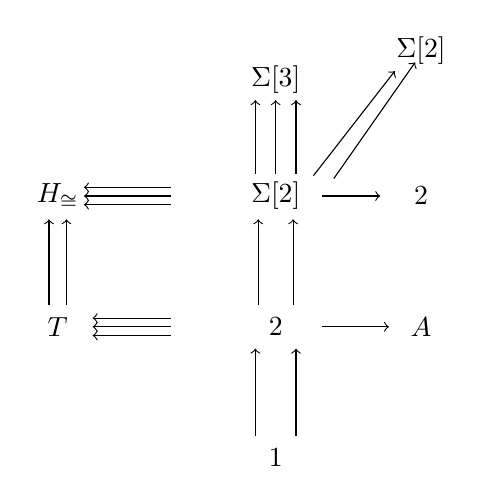
\begin{tikzpicture}[x=1.05em,y=1.05em]
  \node (S3) at (1.0,7.0)   {$\Sigma[3]$};
  \node (S2t) at (6.0,8.0)  {$\Sigma[2]$};
  \node (Ed) at (-6.5,3.0)  {$\mathbb{H}_{\cong}$};
  \node (S2) at (1.0,3.0)   {$\Sigma[2]$};
  \node (tw) at (6.0,3.0)   {$2$};
  \node (tr) at (-6.5,-1.5) {$\mathbb{T}$};
  \node (tc) at (1.0,-1.5)  {$2$};
  \node (on) at (6.0,-1.5)  {$\mathbb{A}$};
  \node (ob) at (1.0,-6.0)  {$1$};
  \draw[->] (0.3,3.75) -- (0.3,6.3);
  \draw[->] (1.0,3.75) -- (1.0,6.3);
  \draw[->] (1.7,3.75) -- (1.7,6.3);
  \draw[->] (2.3,3.7) -- (5.1,7.3);
  \draw[->] (3.0,3.6) -- (5.8,7.6);
  \draw[->] (-2.6,3.3) -- (-5.6,3.3);
  \draw[->] (-2.6,3.0) -- (-5.6,3.0);
  \draw[->] (-2.6,2.7) -- (-5.6,2.7);
  \draw[->] (2.6,3.0) -- (4.6,3.0);
  \draw[->] (-6.8,-0.75) -- (-6.8,2.2);
  \draw[->] (-6.2,-0.75) -- (-6.2,2.2);
  \draw[->] (-2.6,-1.8) -- (-5.3,-1.8);
  \draw[->] (-2.6,-1.5) -- (-5.3,-1.5);
  \draw[->] (-2.6,-1.2) -- (-5.3,-1.2);
  \draw[->] (0.4,-0.75) -- (0.4,2.2);
  \draw[->] (1.6,-0.75) -- (1.6,2.2);
  \draw[->] (2.6,-1.5) -- (4.9,-1.5);
  \draw[->] (0.3,-5.25) -- (0.3,-2.25);
  \draw[->] (1.7,-5.25) -- (1.7,-2.25);
\end{tikzpicture}
\end{center}
其中
\begin{center}
\begin{tikzpicture}[x=1.05em,y=1.05em]
  \node at (-9.5,0.4) {$\mathbb{T}\coloneqq$};
  \node (a) at (-4.5,1.4) {$\bullet$};
  \node (b) at (-6.5,-1.2) {$\bullet$};
  \node (c) at (-2.0,-1.2) {$\bullet$};
  \draw[->] (-5.0,0.8) -- (-6.1,-0.6);
  \draw[->] (-4.0,0.8) -- (-2.6,-0.6);
  \node at (-5.9,0.1) {$\scriptstyle\cong$};
  \draw[->] (-5.9,-1.2) -- (-2.7,-1.2);
  \node at (-0.9,0.4) {，};
  \node at (0.4,0.4) {$\mathbb{A}\coloneqq$};
  \node (d) at (3.2,0.1) {$\bullet$};
  \draw[->] (3.2,0.75) arc[start angle=110,end angle=430,radius=0.62];
  \node at (4.6,0.75) {$\scriptstyle\cong$};
  \node at (5.6,0.4) {，$\Sigma2\coloneqq$};
  \node (e) at (9.0,0.1) {$\bullet$};
  \node (f) at (12.2,0.1) {$\bullet$};
  \draw[->] (9.4,0.45) to[bend left=18] (11.8,0.45);
  \draw[->] (9.4,-0.25) to[bend right=18] (11.8,-0.25);
  \node at (10.6,0.35) {$\scriptstyle\Downarrow$};
  \node at (13.3,0.4) {，$\Sigma[3]\coloneqq$};
  \node (g) at (17.4,0.1) {$\bullet$};
  \node (h) at (20.6,0.1) {$\bullet$};
  \draw[->] (17.8,0.45) to[bend left=18] (20.2,0.45);
  \draw[->] (17.8,-0.25) to[bend right=18] (20.2,-0.25);
  \node at (19.0,0.55) {$\scriptstyle\Downarrow$};
  \node at (19.0,-0.45) {$\scriptstyle\Downarrow$};
  \node at (21.6,0.4) {，};
\end{tikzpicture}
\end{center}
\begin{center}
\begin{tikzpicture}[x=1.05em,y=1.05em]
  \node at (-7.2,0.4) {$\mathbb{H}_{=}\coloneqq$};
  \node (a) at (-3.4,0.1) {$\bullet$};
  \node (b) at (-0.6,0.1) {$\bullet$};
  \node (c) at (2.2,0.1) {$\bullet$};
  \draw[->] (-3.0,0.45) to[bend left=18] (-1.0,0.45);
  \draw[->] (-3.0,-0.25) to[bend right=18] (-1.0,-0.25);
  \node at (-2.0,0.35) {$\scriptstyle\Downarrow$};
  \draw[->] (-0.2,0.45) to[bend left=18] (1.8,0.45);
  \draw[->] (-0.2,-0.25) to[bend right=18] (1.8,-0.25);
  \node at (0.8,0.35) {$\scriptstyle\Downarrow$};
  \node at (3.3,0.4) {，};
  \node at (4.6,0.4) {以及};
  \node at (7.4,0.4) {$\mathbb{H}_{\cong}\coloneqq$};
  \node (d) at (10.6,0.1) {$\bullet$};
  \node (e) at (13.4,0.1) {$\bullet$};
  \node (f) at (16.2,0.1) {$\bullet$};
  \draw[->] (11.0,0.45) to[bend left=18] (13.0,0.45);
  \draw[->] (11.0,-0.25) to[bend right=18] (13.0,-0.25);
  \node at (12.0,0.35) {$\scriptstyle\Downarrow$};
  \draw[->] (13.8,0.45) to[bend left=18] (15.8,0.45);
  \draw[->] (13.8,-0.25) to[bend right=18] (15.8,-0.25);
  \node at (14.8,0.35) {$\scriptstyle\Downarrow$};
  \draw[->] (11.0,0.9) to[bend left=38] (15.8,0.9);
  \node at (13.4,2.5) {$\scriptstyle\cong$};
  \draw[->] (11.0,-0.7) to[bend right=38] (15.8,-0.7);
  \node at (13.4,-2.4) {$\scriptstyle\cong$};
\end{tikzpicture}
\end{center}
它们都是由所描绘的数据生成的自由 2-\trCategory。图表 $D_{2\text{-}\mathcal{C}at}$ 可以
理解为 $E_{2\text{-}\mathcal{C}at}$ 相对于 Lack 的 2-\trCategory{}模型结构（见定理
C.5.14）的一个 Reedy 余纤维性替换，在该模型结构中，余纤维化是那些在对象与
1-\trCell{}上均为单射的 2-\trFunctor，而平凡纤维化则是满射等价 [71]。
\end{example}

从 $E_{2\text{-}\mathcal{C}at}$ 或从 $D_{2\text{-}\mathcal{C}at}$ 映出便定义诸\trFunctor
$N_{-}$ 与 $M_{-}\colon 2\text{-}\Cat\to\Set^{\mathcal{J}_{2\text{-}\mathcal{C}at}}$，其像位于
$\mathcal{J}_{2\text{-}\mathcal{C}at}$-结构的满子\trCategory{}之中。\footnote{同样地，各
图表在全部四个关系符号处的\trLatchingMap{}都是\trEpimorphism。}我们把 $M_{\mathcal{C}}$ 称为
配属于一个 2-\trCategory{} $\mathcal{C}$ 的「饱和」$\mathcal{J}_{2\text{-}\mathcal{C}at}$-结构，
而把 $N_{\mathcal{C}}$ 称为「朴素」$\mathcal{J}_{2\text{-}\mathcal{C}at}$-结构。

\begin{observation}[匹配映射的纤维]\label{obs:matching-maps}
对每个 $\mathcal{J}$-结构 $M\colon\mathcal{J}\to\Set$ 与对象 $K\in\mathcal{J}$——无论
其为一个种类还是一个关系符号——都存在一个典范的\textbf{匹配映射}（matching map）
\begin{center}
\begin{tikzpicture}[x=1.05em,y=1.05em]
  \node (MK) at (0,0.9) {$MK$};
  \node (prod) at (9.5,0.9)
    {$\displaystyle\prod_{p\colon K\to^{\neq}K_{p}} MK_{p}$};
  \node (lim) at (4.2,-1.3)
    {$\partial^{K}M\coloneqq\displaystyle\lim_{p\colon K\to^{\neq}K_{p}} MK_{p}$};
  \draw[->] (1.3,0.9) -- (6.6,0.9);
  \draw[->,dashed] (0.5,0.3) -- (2.9,-0.7);
  \node at (0.9,-0.55) {$\scriptstyle m^{K}$};
  \draw[right hook->] (6.0,-0.9) -- (8.3,0.35);
\end{tikzpicture}
\end{center}
其余定义域是观察 C.1.18 所定义的匹配对象。注意，极限与积都取遍以 $K$ 为定义域的
非恒同箭头——这一隐含条件也适用于下文的类似构造。我们把一个 $\mathcal{J}$-结构
$M$ 设想为一种结构化的集合：其中每个集合 $MK$ 都被进一步分割为匹配映射
$m^{K}\colon MK\to\partial^{K}M$ 的诸\trFiber。
\end{observation}

现在我们来描述 Makkai 的「依赖排序」——它们与其变量一道经由相互递归得到定义。
这些变量可以纯粹以句法方式引入，但我们发现更直观的做法是把它们设想为属于一个%
\textbf{上下文}（context）：此即一个 $\mathcal{J}$-结构 $\Gamma$，其中与每个种类
$K\in\mathcal{J}$ 相关联的集合 $\Gamma K$ 两两不交。

\begin{definition}[排序及其变量]\label{def:sorts-variables}
取定一个 FOLDS 签名 $\mathcal{J}$ 与一个上下文 $\Gamma\colon\mathcal{J}\to\Set$。
\begin{itemize}
\item 每个次数为零的种类 $K$ 都定义一个\textbf{排序}，亦记作 $K$，其变量就是集合
  $\Gamma K$ 的元素。书写「$x:K$」意谓 $x\in\Gamma K$，即 $x$ 是属于上下文 $\Gamma$
  中排序 $K$ 的一个变量。
\item 对每个次数为一的种类 $K$，匹配映射 $m^{K}$ 取下示之形，其中积取遍
  $\mathcal{J}$ 中以 $K$ 为定义域、余定义域次数为零的那些箭头。对任何变量族
  $\{x_{p}\mathbin{:}K_{p}\}_{p\colon K\to^{\neq}K_{p}}$，就有排序 $K\langle x_{p}\rangle$：
  其变量是纤维
\begin{center}
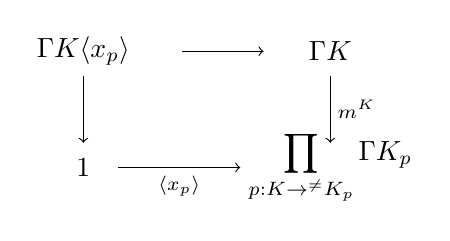
\begin{tikzpicture}[x=1.05em,y=1.05em]
  \node (tl) at (0,3)   {$\Gamma K\langle x_{p}\rangle$};
  \node (tr) at (8.5,3) {$\Gamma K$};
  \node (bl) at (0,-1)  {$1$};
  \node (br) at (8.5,-1)
    {$\displaystyle\prod_{p\colon K\to^{\neq}K_{p}}\Gamma K_{p}$};
  \draw[->] (3.4,3) -- (6.2,3);
  \draw[->] (0,2.15) -- (0,-0.15);
  \draw[->] (8.5,2.15) -- (8.5,-0.15);
  \node at (9.4,1.0) {$\scriptstyle m^{K}$};
  \draw[->] (1.2,-1) -- (5.4,-1);
  \node at (3.3,-1.65) {$\scriptstyle\langle x_{p}\rangle$};
  \node at (1.05,2.45) {$\scriptstyle\lrcorner$};
\end{tikzpicture}
\end{center}
  的元素，并且称这些变量\textbf{依赖}于诸变量 $x_{p}:K_{p}$。
\item 对次数更高的种类 $K$，变量族
  $\{x_{p}\mathbin{:}K_{p}(x_{q_{p}})\}_{p\colon K\to^{\neq}K_{p}}$
  是\textbf{相容的}，若 $(x_{p})\in\prod_{p\colon K\to^{\neq}K_{p}}\Gamma K_{p}$ 属于匹配
  对象 $\partial^{K}\Gamma$。在实践中，这意味着列表中较高次的变量按 FOLDS 签名中
  依赖关系所规定的方式依赖于较低次的变量。对任何相容的变量族，都有排序
  $K\langle x_{p}\rangle$：其变量是匹配映射 $m^{K}$ 在
  $\langle x_{p}\rangle\in\partial^{K}\Gamma$ 之上的\trFiber{}的元素
\begin{center}
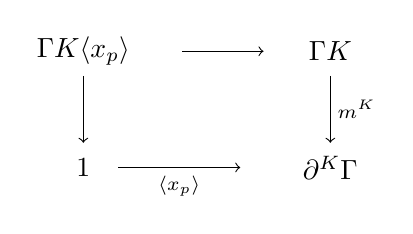
\begin{tikzpicture}[x=1.05em,y=1.05em]
  \node (tl) at (0,3)   {$\Gamma K\langle x_{p}\rangle$};
  \node (tr) at (8.5,3) {$\Gamma K$};
  \node (bl) at (0,-1)  {$1$};
  \node (br) at (8.5,-1) {$\partial^{K}\Gamma$};
  \draw[->] (3.4,3) -- (6.2,3);
  \draw[->] (0,2.15) -- (0,-0.15);
  \draw[->] (8.5,2.15) -- (8.5,-0.15);
  \node at (9.4,1.0) {$\scriptstyle m^{K}$};
  \draw[->] (1.2,-1) -- (5.4,-1);
  \node at (3.3,-1.65) {$\scriptstyle\langle x_{p}\rangle$};
  \node at (1.05,2.45) {$\scriptstyle\lrcorner$};
\end{tikzpicture}
\end{center}
\end{itemize}

按照约定，在排序的规约中显式列出的变量只有最高次的那些变量；这些变量所依赖的
较低次变量，则可从最高次变量所属的排序推得。
\end{definition}

\begin{example}\label{exa:sorts-jcat}
对 FOLDS 签名 $\mathcal{J}_{\mathcal{C}at}$ 而言：
\begin{itemize}
\item 有一个排序 $O$。
\item 对任何一对变量 $x$ 与 $y:O$，有一个排序 $A(x,y)$。
\end{itemize}
\end{example}

\begin{example}\label{exa:sorts-j2cat}
对 FOLDS 签名 $\mathcal{J}_{2\text{-}\mathcal{C}at}$ 而言：
\begin{itemize}
\item 有一个排序 $C_{0}$。
\item 对任何一对变量 $x$ 与 $y:C_{0}$，有一个排序 $C_{1}(x,y)$。
\item 对任何 $x$ 与 $y:C_{0}$、以及 $f$ 与 $g:C_{1}(x,y)$，有一个排序
  $C_{2}(x,y,f,g)$。这个排序通常缩写作 $C_{2}\langle f,g\rangle$，其隐含变量
  $x$ 与 $y:C_{0}$ 可由变量 $f$ 与 $g$ 所居住的排序推知。
\end{itemize}
\end{example}

沿用同样的缩写：
\begin{itemize}
\item 对任何 $x:C_{0}$ 与 $f:C_{1}(x,x)$，有一个排序 $I_{1}(f)$。
\item 对任何 $x$、$y$、$z:C_{0}$ 以及 $f:C_{1}(x,y)$、$g:C_{1}(y,z)$ 与
  $h:C_{1}(x,z)$，有一个排序 $T\langle f,g,h\rangle$。
\end{itemize}

我们现在已准备好引入与一个 FOLDS 签名 $\mathcal{J}$ 相关联的形式语言的公式与语句。
它们由递归定义，从原子公式出发，而原子公式由诸关系符号支配。再次取定一个 FOLDS
签名 $\mathcal{J}$ 与一个上下文 $\Gamma\colon\mathcal{J}\to\Set$。

\begin{definition}\label{def:atomic-formula}
带依赖排序的逻辑中的一个\textbf{原子公式}（atomic formula）是形如
$\dot{R}\langle x_{p}\rangle$ 的一个实体，其中 $\dot{R}$ 是一个关系符号，而变量
$\{x_{p}\mathbin{:}K_{p}(x_{q_{p}})\}_{p\colon \dot{R}\to^{\neq}K_{p}}$
必须定义一个相容族，意即它们定义了一个元素
$\langle x_{p}\rangle\in\partial^{\dot{R}}\Gamma$。
\end{definition}

\begin{example}\label{exa:atomic-formula-commutative-triangle}
在 FOLDS 签名 $\mathcal{J}_{\mathcal{C}at}$ 中，对任何 $x$、$y$、$z:O$ 以及
$f:A(x,y)$、$g:A(y,z)$ 与 $h:A(x,z)$，都有一个原子公式
$\dot{T}\langle x,y,z,f,g,h\rangle$，缩写作 $\dot{T}\langle f,g,h\rangle$，它可以被
设想为断言由箭头 $f$、$g$ 与 $h$ 构成的三角形的交换性。
\end{example}

\begin{digression}\label{dig:restricted-equality}
FOLDS 哲学的一个关键想法是：它应当表达一种带受限相等性的逻辑。这一点在 FOLDS
签名 $\mathcal{J}_{\mathcal{C}at}$ 与 $\mathcal{J}_{2\text{-}\mathcal{C}at}$ 中清晰可见：
二者在种类 $A$ 与 $C_{2}$ 上包含二元相等关系符号，但在这些种类所依赖的种类
$O$、$C_{0}$ 与 $C_{1}$ 上却不配备类似的相等谓词。更精确地说，$\mathcal{J}_{\mathcal{C}at}$
的原子公式 $\dot{E}(f,g)$ 与 $\mathcal{J}_{2\text{-}\mathcal{C}at}$ 的原子公式
$\dot{E}(\alpha,\beta)$ 可用于表达一对平行箭头的相等，因为相容性要求对某对
$x$ 与 $y:O$ 有 $f$ 与 $g:A(x,y)$；亦可用于表达平行 2-\trCell{}的相等，因为相容性
要求对某对 $f$ 与 $g:C_{1}(x,y)$ 及某对 $x$ 与 $y:C_{0}$\footnote{原书此两处分别
印作「$\alpha,\beta:C_{1}\langle f,g\rangle$」与「$x,y:O$」（2026-09-15 机械
波次经 booktext 文本层复核证实，唯原引录括号有误，径正）。按例 11.2.11 所立
之排序口径，平行 2-\trCell{}居于排序 $C_{2}\langle f,g\rangle$ 之中，且
$C_{1}(x,y)$ 要求 $x,y:C_{0}$，故疑分别系 $C_{2}\langle f,g\rangle$ 与 $C_{0}$
之误，此处径改。——译者注}有 $\alpha$ 与 $\beta:C_{2}\langle f,g\rangle$。这种限制对主要定理而言
是本质性的：以给定签名的 FOLDS 语言所表达的语句之有效性，在诸结构之间适当定义的%
\trEquivalence{}之下不变。
\end{digression}

在 FOLDS 中，全称量化或存在量化都只能对某个指定排序中的变量进行，前提是所论
谓词中的变量不依赖于被量化的变量。

\begin{definition}\label{def:formulae}
\textbf{公式}（formula）$\phi$ 及其\textbf{自由变量}（free variables）之集
$\mathrm{var}(\phi)$ 由同时递归定义：
\begin{itemize}
\item 一个原子公式是一个公式。$\dot{R}\langle x_{p}\rangle$ 的变量就是诸 $x_{p}$。
\end{itemize}
复合公式则由其他公式经下列步骤归纳地定义：
\begin{itemize}
\item $\top$ 与 $\bot$ 都是公式，且
  $\mathrm{var}(\top)\coloneqq\mathrm{var}(\bot)\coloneqq\varnothing$。
\item 公式可以经语句联结词 $\wedge$、$\vee$ 与 $\rightarrow$ 加以组合，此时变量经
  并集而组合：例如 $\mathrm{var}(\phi\wedge\psi)=\mathrm{var}(\phi)\cup\mathrm{var}(\psi)$。
\item 当 $\phi$ 是一个公式而 $x$ 是一个变量，使得 $\mathrm{var}(\phi)$ 中没有变量
  依赖于 $x$——尽管容许 $x\in\mathrm{var}(\phi)$——那么 $\forall x\,\phi$ 与
  $\exists x\,\phi$ 就是良构公式\footnote{正如我们在例子中所展示的，完整的语法
  要求每个被量化的变量都连同其排序一道声明，以此表达量化的范围。}，其变量由
  集合
\begin{equation*}
\mathrm{var}(\forall x\,\phi)\coloneqq\mathrm{var}(\exists x\,\phi)\coloneqq
(\mathrm{var}(\phi)-\{x\})\cup\mathrm{dep}(x)
\end{equation*}
  给出——此集合由「从 $\phi$ 的变量中删去 $x$（若其出现）、再添上 $x$ 所依赖的
  全部变量（若其尚未出现）」而形成。
\end{itemize}
当一个公式中的变量之集为空时，我们称该公式为一个\textbf{语句}。
\end{definition}

一个 $\mathcal{J}$-上下文 $\Gamma$ 在一个 $\mathcal{J}$-结构 $M$ 中的\textbf{求值}
（evaluation）由一个\trNaturalTransformation{} $\alpha\colon\Gamma\to M$ 给出，后者
定义了其变量的一个解释，把变量 $x:K\langle x_{p}\rangle$ 送到映射
$MK\to\partial^{K}M$ 在 $\langle\alpha x_{p}\rangle$ 之上的\trFiber{}中的一个元素。
要解释一个具体的公式 $\phi$，无须指定整个上下文 $\Gamma$ 的解释；只需指定其变量
$\mathrm{var}(\phi)\subset\Gamma$ 的解释即可，而后者本身又可以被视为一个上下文
（见\cref{ex:var-subcontext}）。

按公式复杂度归纳地，我们定义：一个 $\mathcal{J}$-结构 $M$ 在其变量的一个给定解释
$\alpha\colon\mathrm{var}(\phi)\to M$ 之下\textbf{满足}（satisfy）一个公式 $\phi$
意谓什么——我们把这一性质记作 $M\models\phi[\alpha]$。

\begin{definition}\label{def:satisfies-atomic}
一个 $\mathcal{J}$-结构 $M$ 在一个解释 $\alpha$ 之下\textbf{满足}一个原子公式
$\dot{R}\langle x_{p}\rangle$，当且仅当元组
$\langle\alpha x_{p}\rangle\in\prod_{p\colon \dot{R}\to^{\neq}K_{p}}MK_{p}$ 位于子集
$M\dot{R}$ 之中；此时写作 $M\models\dot{R}[\alpha]$。
\end{definition}

语句 $\top$ 与 $\bot$ 没有变量，故其语义独立于解释。任何 $\mathcal{J}$-结构都满足
$\top$，且没有 $\mathcal{J}$-结构满足 $\bot$。

\begin{definition}\label{def:satisfies-compound}
一个 $\mathcal{J}$-结构 $M$ 在解释
$\alpha\colon\mathrm{var}(\phi)\cup\mathrm{var}(\psi)\to M$ 之下满足由 $\phi$ 与
$\psi$ 构造的复合公式，依如下规则：
\begin{itemize}
\item $M\models(\phi\wedge\psi)[\alpha]$ 当且仅当 $M\models\phi[\alpha]$ 且
  $M\models\psi[\alpha]$；
\item $M\models(\phi\vee\psi)[\alpha]$ 当且仅当 $M\models\phi[\alpha]$ 或
  $M\models\psi[\alpha]$；
\item $M\models(\phi\rightarrow\psi)[\alpha]$ 当且仅当：只要
  $M\models\phi[\alpha]$，则也有 $M\models\psi[\alpha]$。
\end{itemize}
\end{definition}

\begin{definition}\label{def:satisfies-forall}
考虑一个公式 $\forall x\,\phi$，其中 $x:K\langle x_{p}\rangle$，连同其一个解释
\begin{equation*}
\alpha\colon\mathrm{var}(\forall x\,\phi)\to M
\end{equation*}
在一个 $\mathcal{J}$-结构 $M$ 中；注意 $x\notin\mathrm{var}(\forall x\,\phi)$，故这并
未给出变量 $x$ 自身的解释。我们说 $M$ 在解释 $\alpha$ 之下\textbf{满足}
$\forall x\,\phi$，若对映射 $MK\to\partial^{K}M$ 在 $\langle\alpha x_{p}\rangle$ 之上的%
\trFiber{}中的所有 $a$，都有 $M\models\phi(a/x)[\alpha]$。也就是说，
$M\models\forall x\,\phi[\alpha]$，若任何具有恰当依赖关系的 $a$ 都能替换到解释中的
$\phi$ 里顶替 $x$，从而得到一个 $M$ 所满足的公式。

类似地，$M$ 在解释 $\alpha$ 之下\textbf{满足} $\exists x\,\phi$，若在映射
$MK\to\partial^{K}M$ 于 $\langle\alpha x_{p}\rangle$ 之上的\trFiber{}中存在某个
$a$，使得 $M\models\phi(a/x)[\alpha]$。也就是说，$M\models\exists x\,\phi[\alpha]$，
若某个具有恰当依赖关系的 $a$ 能替换到解释中的 $\phi$ 里顶替 $x$，从而得到一个
$M$ 所满足的公式。
\end{definition}

\begin{example}\label{exa:isomorphism-sentence-jcat}
在 $\mathcal{J}_{\mathcal{C}at}$ 的语言中，在由 $x$ 与 $y:O$ 给出的上下文中，公式
\begin{equation*}
\begin{aligned}
\exists f&:A(x,y),\ \exists g:A(y,x),\ \forall 1_{x}:A(x,x),\
\forall 1_{y}:A(y,y),\\
&(\dot{I}\langle 1_{x}\rangle\wedge\dot{I}\langle 1_{y}\rangle)
\to(\dot{T}\langle f,g,1_{x}\rangle\wedge\dot{T}\langle g,f,1_{y}\rangle)
\end{aligned}
\end{equation*}
断言：在一个解释所指定的两个对象之间存在一个\trIsomorphism。
\end{example}

\begin{example}\label{exa:equivalence-sentence-j2cat}
除记号改动外，在 $\mathcal{J}_{2\text{-}\mathcal{C}at}$ 的语言中也有一个类似的语句，
其上下文由 $x$ 与 $y:C_{0}$ 给出：
\begin{equation*}
\begin{aligned}
\exists f&:C_{1}(x,y),\ \exists g:C_{1}(y,x),\ \forall 1_{x}:C_{1}(x,x),\
\forall 1_{y}:C_{1}(y,y),\\
&\forall\mu:I_{1}\langle 1_{x}\rangle,\ \forall\nu:I_{1}\langle 1_{y}\rangle,\
\exists\alpha:T\langle f,g,1_{x}\rangle\wedge\exists\beta:T\langle g,f,1_{y}\rangle
\end{aligned}
\end{equation*}
其中「$\exists\alpha:T\langle f,g,1_{x}\rangle$」是公式
「$\exists\alpha:T\langle f,g,1_{x}\rangle.\top$」的缩写。

在配属于一个 2-\trCategory{} $\mathcal{C}$ 的朴素
$\mathcal{J}_{2\text{-}\mathcal{C}at}$-结构 $N_{\mathcal{C}}$ 中，该解释同样给出所指定
对象之间的一个\trIsomorphism；但在\cref{exa:e-d-functors-2cat}中定义的饱和
$\mathcal{J}_{2\text{-}\mathcal{C}at}$-结构 $M_{\mathcal{C}}$ 中，该解释现在给出的则是一
个\trEquivalence。由\cref{exa:pseudo-comma-2-category}的构造，在
$\mathcal{J}_{2\text{-}\mathcal{C}at}$-结构
$M_{\mathcal{C}}$ 中得到解释的 2-\trCategory{}语言中的诸公式，在 2-\trCategory{}的%
\trBiequivalence{}之下不变，尽管当它们在朴素 $\mathcal{J}_{2\text{-}\mathcal{C}at}$-结构
$N_{\mathcal{C}}$ 中得到解释时，这一结果未必成立（见\cref{ex:naive-not-j-equivalent}与题外话 B.1.7）。
\end{example}

我们现给出一个判据，保证两个 $\mathcal{J}$-结构满足同样的公式。

\begin{definition}\label{def:fiberwise-surjective}
诸 $\mathcal{J}$-结构之间的一个\trNaturalTransformation{} $\rho\colon M\to N$ 是%
\textbf{逐纤维满的}（fiberwise surjective），若对每个 $K\in\mathcal{J}$——无论其为
关系符号还是种类——映到\trPullback
\begin{rveq}\label{eq:matching-square}
\vcenter{\hbox{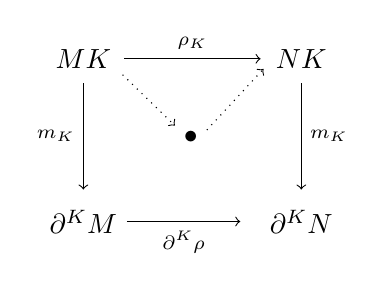
\begin{tikzpicture}[x=1.05em,y=1.05em]
  \node (tl) at (0,3)    {$MK$};
  \node (tr) at (7.5,3)  {$NK$};
  \node (bl) at (0,-2.6) {$\partial^{K}M$};
  \node (br) at (7.5,-2.6) {$\partial^{K}N$};
  \node (pb) at (3.7,0.3) {$\bullet$};
  \draw[->] (1.4,3) -- node[above]{$\scriptstyle\rho_{K}$} (6.1,3);
  \draw[->] (0,2.15) -- (0,-1.5);
  \node at (-0.95,0.35) {$\scriptstyle m_{K}$};
  \draw[->] (7.5,2.15) -- (7.5,-1.5);
  \node at (8.45,0.35) {$\scriptstyle m_{K}$};
  \draw[->] (1.5,-2.6) -- node[below]{$\scriptstyle\partial^{K}\rho$} (5.4,-2.6);
  \draw[->,dotted] (1.35,2.45) -- (3.15,0.7);
  \draw[->,dotted] (4.25,0.55) -- (6.2,2.65);
  \node at (4.9,-0.5) {$\scriptstyle\lrcorner$};
\end{tikzpicture}}}
\end{rveq}
的映射，在 $K$ 的「匹配方块」（matching square）中是一个\trEpimorphism。
\end{definition}

用 C.5 节的术语来说，逐纤维满的映射恰是那些定义\textbf{Reedy \trEpimorphism}的%
\trNaturalTransformation——即那些相对匹配映射 \eqref{eq:matching-square} 为%
\trEpimorphism{}的\trNaturalTransformation。

\begin{lemma}\label{lem:matching-square-pullback}
设 $\rho\colon M\to N$ 是诸 $\mathcal{J}$-结构之间的一个逐纤维满射（fiberwise
surjection）。那么对每个关系
符号 $\dot{R}$，匹配方块是一个\trPullback：
\begin{center}
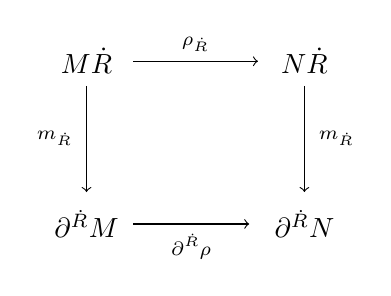
\begin{tikzpicture}[x=1.05em,y=1.05em]
  \node (tl) at (0,3)    {$M\dot{R}$};
  \node (tr) at (7.5,3)  {$N\dot{R}$};
  \node (bl) at (0,-2.6) {$\partial^{\dot{R}}M$};
  \node (br) at (7.5,-2.6) {$\partial^{\dot{R}}N$};
  \draw[->] (1.6,3) -- node[above]{$\scriptstyle\rho_{\dot{R}}$} (5.9,3);
  \draw[->] (0,2.15) -- (0,-1.5);
  \node at (-1.1,0.35) {$\scriptstyle m_{\dot{R}}$};
  \draw[->] (7.5,2.15) -- (7.5,-1.5);
  \node at (8.6,0.35) {$\scriptstyle m_{\dot{R}}$};
  \draw[->] (1.6,-2.6) -- node[below]{$\scriptstyle\partial^{\dot{R}}\rho$} (5.6,-2.6);
  \node at (1.05,2.45) {$\scriptstyle\lrcorner$};
\end{tikzpicture}
\end{center}
\end{lemma}

\begin{proof}
由于 $M$ 与 $N$ 都是 $\mathcal{J}$-结构，$\mathcal{J}$ 的诸关系符号的匹配映射都是%
\trMonomorphism{}（见\cref{ex:folds-matching-map-mono}）。于是，到该\trPullback{}的诱导映射是一个%
\trMonomorphism，而由逐纤维满性假设，它又是一个\trEpimorphism。于是，这个映射
是集合\trCategory{}中的一个\trIsomorphism，故该方块是一个\trPullback。
\end{proof}

请回忆\cref{exa:d-cat-nerve}与\cref{exa:e-d-functors-2cat}中构造的那些结构。

\begin{lemma}\label{lem:surjective-equivalence-fiberwise-surjection}
\begin{enumerate}[label=(\roman*)]
\item \trCategory{}之间的一个\trSurjectiveEquivalence{}
$\mathcal{C}\Rightarrow\mathcal{D}$ 诱导诸 $\mathcal{J}_{\mathcal{C}at}$-结构之间的一个
逐纤维满射 $M_{\mathcal{C}}\Rightarrow M_{\mathcal{D}}$。
\item 2-\trCategory{}之间的一个满射\trBiequivalence{}
$\mathcal{C}\Rightarrow\mathcal{D}$ 诱导诸 $\mathcal{J}_{2\text{-}\mathcal{C}at}$-结构
之间的一个逐纤维满射 $M_{\mathcal{C}}\Rightarrow M_{\mathcal{D}}$。
\end{enumerate}
\end{lemma}

\begin{proof}
这两个陈述是某个更一般的结果的特殊情形，因而有一个公共的证明 [52]。在 $\Cat$ 与
$2\text{-}\Cat$ 上各有一个（余纤维化，平凡纤维化）弱分解系统，其平凡纤维化即陈述中
所指的那些满射双／等价。这些结构是经由应用如下 hom-\trBifunctor{}而定义的
\begin{equation*}
(\Cat^{\mathcal{J}_{\mathcal{C}at}^{\mathrm{op}}})^{\mathrm{op}}\times\Cat
\xrightarrow{\ \mathrm{hom}\ }\Set^{\mathcal{J}_{\mathcal{C}at}}
\qquad\qquad
(2\text{-}\Cat^{\mathcal{J}_{2\text{-}\mathcal{C}at}^{\mathrm{op}}})^{\mathrm{op}}
\times 2\text{-}\Cat
\xrightarrow{\ \mathrm{hom}\ }\Set^{\mathcal{J}_{2\text{-}\mathcal{C}at}}
\end{equation*}
到那些为 Reedy 余纤维性的图表 $D_{\mathcal{C}at}$ 与 $D_{2\text{-}\mathcal{C}at}$ 上。由引理
C.2.11 与推论 C.5.16，相对于由 $\Cat$ 与 $2\text{-}\Cat$ 上的任一弱分解系统以及
$\Set$ 上的（单态射，满态射）弱分解系统所构建的诸 Reedy 弱分解系统，它们都是右
Leibniz 二函子，因为它们是涉及（未富集的）加权余极限二函子的一个双变量伴随中的
右\trAdjunction{}之各项。于是，诸\trFunctor{}
$M_{-}\colon\Cat\to\Set^{\mathcal{J}_{\mathcal{C}at}}$ 与
$M_{-}\colon 2\text{-}\Cat\to\Set^{\mathcal{J}_{2\text{-}\mathcal{C}at}}$ 把平凡纤维化
——即满射双／等价——送到 Reedy \trEpimorphism，即逐纤维满射。
\end{proof}

\begin{definition}\label{def:j-equivalent-in-context}
设 $\mathcal{J}$ 是一个 FOLDS 签名，并设 $\Gamma\colon\mathcal{J}\to\Set$ 是一个带有
给定解释 $\alpha\colon\Gamma\to M$ 与 $\beta\colon\Gamma\to N$ 的上下文，其中
$M,N\colon\mathcal{J}\to\Set$ 为诸 $\mathcal{J}$-结构。诸 $\mathcal{J}$-结构 $M$ 与
$N$ 是\textbf{在上下文 $\Gamma$ 中 $\mathcal{J}$-等价的}（$\mathcal{J}$-equivalent
in context），记作 $M\approx^{\mathcal{J}}_{\Gamma}N$，当且仅当存在一个由 $\Gamma$
之下的诸 $\mathcal{J}$-结构之间的逐纤维满射 $\sigma$ 与 $\rho$ 构成的图表
\begin{center}
\begin{tikzpicture}[x=1.05em,y=1.05em]
  \node (G) at (0,4)   {$\Gamma$};
  \node (M) at (-6,0)  {$M$};
  \node (N) at (6,0)   {$N$};
  \node (P) at (0,-4)  {$P$};
  \draw[->] (-0.95,3.35) -- node[above left,pos=0.45]{$\scriptstyle\alpha$} (-5.2,0.5);
  \draw[->] (0.95,3.35)  -- node[above right,pos=0.45]{$\scriptstyle\beta$} (5.2,0.5);
  \draw[->] (0,3.1)      -- node[right,pos=0.5]{$\scriptstyle\gamma$} (0,-3.1);
  \draw[->] (-0.95,-3.35) -- node[below left,pos=0.55]{$\scriptstyle\sigma$} (-5.2,-0.5);
  \draw[->] (0.95,-3.35)  -- node[below right,pos=0.55]{$\scriptstyle\rho$} (5.2,-0.5);
\end{tikzpicture}
\end{center}
关系「在上下文 $\Gamma$ 中 $\mathcal{J}$-等价」显然是自反的与对称的。事实上，它
也是传递的，读者可在\cref{ex:j-equivalence-transitive}中予以验证。
\end{definition}

\begin{example}\label{exa:jcat-equivalence-iso-comma}
考虑\trCategory{}之间的一个\trEquivalence{} $f\colon\mathcal{C}\to\mathcal{D}$，并经
如下\trPullback{}作出\cref{def:iso-commas}的\trIsoCommaCategory，
\begin{center}
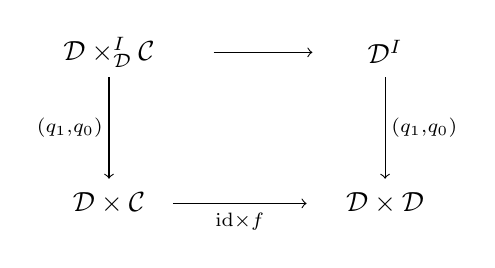
\begin{tikzpicture}[x=1.05em,y=1.05em]
  \node (tl) at (0,2.6)    {$\mathcal{D}\times^{\hciso}_{\mathcal{D}}\mathcal{C}$};
  \node (tr) at (9.5,2.6)  {$\mathcal{D}^{\hciso}$};
  \node (bl) at (0,-2.6)   {$\mathcal{D}\times\mathcal{C}$};
  \node (br) at (9.5,-2.6) {$\mathcal{D}\times\mathcal{D}$};
  \draw[->] (3.6,2.6) -- (7.0,2.6);
  \draw[->] (0,1.75) -- (0,-1.75);
  \node at (-1.35,0) {$\scriptstyle(q_{1},q_{0})$};
  \draw[->] (9.5,1.75) -- (9.5,-1.75);
  \node at (10.85,0) {$\scriptstyle(q_{1},q_{0})$};
  \draw[->] (2.2,-2.6) -- node[below]{$\scriptstyle\mathrm{id}\times f$} (6.8,-2.6);
  \node at (1.05,2.0) {$\scriptstyle\lrcorner$};
\end{tikzpicture}
\end{center}
由于 $f$ 是\trCategory{}之间的一个\trEquivalence，函子
\begin{equation*}
\mathcal{D}\xleftarrow{\ q_{1}\ }
\mathcal{D}\times^{\hciso}_{\mathcal{D}}\mathcal{C}
\xrightarrow{\ q_{0}\ }\mathcal{C}
\end{equation*}
都是\trSurjectiveEquivalence。由\cref{lem:surjective-equivalence-fiberwise-surjection}，%
\cref{exa:d-cat-nerve}的那些朴素 $\mathcal{J}_{\mathcal{C}at}$-结构之间相应的%
\trNaturalTransformation{}是逐纤维满射
\begin{center}
\begin{tikzpicture}[x=1.05em,y=1.05em]
  \node (Mt) at (0,3)   {$M_{\mathcal{D}\times^{\hciso}_{\mathcal{D}}\mathcal{C}}$};
  \node (Ml) at (-6.5,-1) {$M_{\mathcal{C}}$};
  \node (Mr) at (6.5,-1)  {$M_{\mathcal{D}}$};
  \draw[->] (-2.1,2.4) -- node[above left,pos=0.4]{$\scriptstyle q_{0}$} (-5.3,-0.4);
  \draw[->] (2.1,2.4)  -- node[above right,pos=0.4]{$\scriptstyle q_{1}$} (5.3,-0.4);
\end{tikzpicture}
\end{center}
从而在 $M_{\mathcal{C}}$ 与 $M_{\mathcal{D}}$ 之间定义了一个
$\mathcal{J}_{\mathcal{C}at}$-等价。
\end{example}

\begin{example}\label{exa:pseudo-comma-2-category}
考虑 2-\trCategory{}之间的一个\trBiequivalence{} $F\colon\mathcal{C}\to\mathcal{D}$，并
作出\textbf{伪逗号 2-\trCategory}（pseudo-comma 2-category）$\mathcal{P}$，其
\begin{itemize}
\item 对象是三元组 $(x\in\mathcal{C},\,x'\in\mathcal{D},\,a:Fx\simeq x'\in\mathcal{D})$，
  其中 $a$ 是 $\mathcal{D}$ 中的一个\trEquivalence；
\item 1-\trCell{} $(x,x',a)\to(y,y',b)$ 是三元组
\begin{equation*}
\left(
\begin{array}{ccccc}
x & & x' & & Fx\xrightarrow{\ \simeq a\ }x'\\
f\downarrow & \in\mathcal{C}, & f'\downarrow & \in\mathcal{D}, &
Ff\downarrow\ \cong\alpha\ \downarrow f'\ \in\mathcal{D}\\
y & & y' & & Fy\xrightarrow{\ \simeq b\ }y'
\end{array}
\right)
\end{equation*}
\item 2-\trCell{} $(f,f',\alpha)\Rightarrow(g,g',\beta)$ 由一个对
  $(\gamma:f\Rightarrow g\in\mathcal{C},\,\delta:f'\Rightarrow g'\in\mathcal{D})$ 给出，
  使得
\begin{equation*}
\left(
\begin{array}{ccc}
Fx & \xrightarrow{\ \simeq a\ } & x'\\
Ff & \begin{matrix}F\gamma\Downarrow\\ \cong\alpha\end{matrix}\ Fg\ \cong\beta & g'\\
Fy & \xrightarrow{\ \simeq b\ } & y'
\end{array}
\right)
=
\left(
\begin{array}{ccc}
Fx & \xrightarrow{\ \simeq a\ } & x'\\
Ff & \cong\alpha\ \ f'\ \ \delta\Downarrow & g'\\
Fy & \xrightarrow{\ \simeq b\ } & y'
\end{array}
\right)
\end{equation*}
\end{itemize}
显然的投射 $\mathcal{C}\leftarrow\mathcal{P}\to\mathcal{D}$ 定义满射%
\trBiequivalence——即那些于对象上为满、于 1-\trCell{}上为满、且于 2-\trCell{}上为
全忠实的 2-\trFunctor——它们由\cref{lem:surjective-equivalence-fiberwise-surjection}诱导%
\cref{exa:e-d-functors-2cat}的那些饱和 $\mathcal{J}_{2\text{-}\mathcal{C}at}$-结构之间的
逐纤维满的\trNaturalTransformation，从而定义一个 $\mathcal{J}_{2\text{-}\mathcal{C}at}$-等价
\begin{center}
\begin{tikzpicture}[x=1.05em,y=1.05em]
  \node (Mt) at (0,3)    {$M_{\mathcal{P}}$};
  \node (Ml) at (-6.5,-1) {$M_{\mathcal{C}}$};
  \node (Mr) at (6.5,-1)  {$M_{\mathcal{D}}$};
  \draw[->] (-1.9,2.4) -- node[above left,pos=0.4]{$\scriptstyle\sigma$} (-5.1,-0.4);
  \draw[->] (1.9,2.4)  -- node[above right,pos=0.4]{$\scriptstyle\rho$} (5.1,-0.4);
\end{tikzpicture}
\end{center}
\end{example}

这两种构造都可以理解为 Brown 分解 C.1.6 应用于 $\Cat$ 与 $2\text{-}\Cat$ 上的%
\trFolkModelStructure{}中的实例。我们对这些概念的兴趣源于 Makkai 的下述定理：

\begin{theorem}\label{thm:makkai-invariance}
若 $M$ 与 $N$ 在一个上下文 $\Gamma$ 中是 $\mathcal{J}$-等价的
\begin{center}
\begin{tikzpicture}[x=1.05em,y=1.05em]
  \node (G) at (0,4)   {$\Gamma$};
  \node (M) at (-6,0)  {$M$};
  \node (N) at (6,0)   {$N$};
  \node (P) at (0,-4)  {$P$};
  \draw[->] (-0.95,3.35) -- node[above left,pos=0.45]{$\scriptstyle\alpha$} (-5.2,0.5);
  \draw[->] (0.95,3.35)  -- node[above right,pos=0.45]{$\scriptstyle\beta$} (5.2,0.5);
  \draw[->] (0,3.1)      -- node[right,pos=0.5]{$\scriptstyle\gamma$} (0,-3.1);
  \draw[->] (-0.95,-3.35) -- node[below left,pos=0.55]{$\scriptstyle\sigma$} (-5.2,-0.5);
  \draw[->] (0.95,-3.35)  -- node[below right,pos=0.55]{$\scriptstyle\rho$} (5.2,-0.5);
\end{tikzpicture}
\end{center}
那么对所有满足 $\mathrm{var}(\phi)\subset\Gamma$ 的公式 $\phi$，
$M\models\phi[\alpha]$ 当且仅当 $N\models\phi[\beta]$。
\end{theorem}

\begin{proof}
由于 $P$ 本身就是一个 $\mathcal{J}$-结构，并配有由该上下文所定义之变量的一个解释
$\gamma\colon\Gamma\to P$，故只需证明：对任何逐纤维满射 $\sigma\colon P\to M$，$P$
与 $M$ 满足同样的公式：$P\models\phi[\gamma]$ 当且仅当 $M\models\phi[\sigma\gamma]$。
这沿公式 $\phi$ 的复杂度作归纳而得证。

对于基础情形，考虑一个在 $P$ 中带有解释 $x_{p}\mapsto\gamma x_{p}$ 的原子公式
$\dot{R}\langle x_{p}\rangle$。由\cref{lem:matching-square-pullback}的\trPullback，
$\langle\gamma x_{p}\rangle\in\partial^{\dot{R}}P$ 位于 $P\dot{R}$ 中，当且仅当
$\langle\gamma x_{p}\rangle\in\partial^{\dot{R}}M$ 位于 $M\dot{R}$ 中。于是，
$P\models\dot{R}[\gamma]$ 当且仅当 $M\models\dot{R}[\sigma\gamma]$。

接下来考虑由 $\phi$ 与 $\psi$ 构造的复合公式 $\phi\wedge\psi$、$\phi\vee\psi$ 与
$\phi\rightarrow\psi$。在归纳假设下，可以假定 $P\models\phi[\gamma]$ 当且仅当
$M\models\phi[\sigma\gamma]$，对 $\psi$ 亦然。于是立得：$P\models(\phi\wedge\psi)[\gamma]$
当且仅当 $M\models(\phi\wedge\psi)[\sigma\gamma]$，对复合公式 $\phi\vee\psi$ 与
$\phi\rightarrow\psi$ 亦然。

最后，考虑形如 $\forall x\,\phi$ 的公式，其中 $x:K\langle x_{p}\rangle$。解释
$\gamma\colon\mathrm{var}(\forall x\,\phi)\to P$ 在匹配对象中定义了一个元素
$\langle\gamma x_{p}\rangle\in\partial^{K}P$。逐纤维满性条件告诉我们：下右所示的
$K$ 的匹配方块中从 $PK$ 到该\trPullback{}的映射是一个满射：
\begin{center}
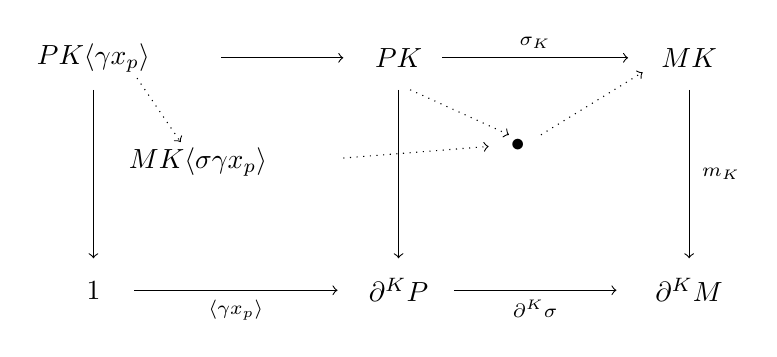
\begin{tikzpicture}[x=1.05em,y=1.05em]
  \node (PKX) at (0,4)     {$PK\langle\gamma x_{p}\rangle$};
  \node (PK)  at (10.5,4)  {$PK$};
  \node (MK)  at (20.5,4)  {$MK$};
  \node (MKX) at (3.6,0.4) {$MK\langle\sigma\gamma x_{p}\rangle$};
  \node (dot) at (14.6,1.0) {$\bullet$};
  \node (one) at (0,-4)    {$1$};
  \node (dKP) at (10.5,-4) {$\partial^{K}P$};
  \node (dKM) at (20.5,-4) {$\partial^{K}M$};
  \draw[->] (4.4,4) -- (8.6,4);
  \draw[->] (12.0,4) -- node[above]{$\scriptstyle\sigma_{K}$} (18.4,4);
  \draw[->] (0,2.9) -- (0,-2.9);
  \draw[->] (10.5,2.9) -- (10.5,-2.9);
  \draw[->] (20.5,2.9) -- (20.5,-2.9);
  \node at (21.6,0) {$\scriptstyle m_{K}$};
  \draw[->] (1.4,-4) -- node[below]{$\scriptstyle\langle\gamma x_{p}\rangle$} (8.4,-4);
  \draw[->] (12.4,-4) -- node[below]{$\scriptstyle\partial^{K}\sigma$} (18.0,-4);
  \draw[->,dotted] (1.5,3.3) -- (3.0,1.1);
  \draw[->,dotted] (8.6,0.55) -- (13.6,0.95);
  \draw[->,dotted] (15.4,1.35) -- (18.9,3.5);
  \draw[->,dotted] (10.9,2.9) -- (14.3,1.35);
  \node at (4.0,4.3) {$\scriptstyle\lrcorner$};
  \node at (8.3,-0.2) {$\scriptstyle\lrcorner$};
  \node at (14.9,0.1) {$\scriptstyle\lrcorner$};
\end{tikzpicture}
\end{center}
通过对\trPullback{}作复合，即得：从 $PK\to\partial^{K}P$ 在 $\langle\gamma x_{p}\rangle$
之上的\trFiber{}到 $MK\to\partial^{K}M$ 在 $\langle\sigma\gamma x_{p}\rangle$ 之上的%
\trFiber{}有一个满射。特别地，若对 $PK\to\partial^{K}P$ 的\trFiber{}中所有 $a$ 都有
$P\models\phi(a/x)[\gamma]$，则由归纳假设 $M\models\phi(\sigma a/x)[\sigma\gamma]$。
由逐纤维满性，$MK\to\partial^{K}M$ 的\trFiber{}中每个元素 $b$ 都等于 $PK\to\partial^{K}P$
的\trFiber{}中某个 $a$ 在 $\sigma$ 下的像，故这告诉我们 $P\models(\forall x\,\phi)[\gamma]$
当且仅当 $M\models(\forall x\,\phi)[\sigma\gamma]$。

类似地，对 $\exists x\,\phi$ 而言，$P\models(\exists x\,\phi)[\gamma]$ 当且仅当在%
\trFiber{}中存在某个 $a$ 使得 $P\models\phi(a/x)[\gamma]$。而这成立当且仅当
$M\models\phi(\sigma a/x)[\sigma\gamma]$，并且由 $\sigma$ 的自然性，$\sigma a$ 居于
恰当的\trFiber{}之中。所以，若 $P\models(\exists x\,\phi)[\gamma]$，则
$M\models(\exists x\,\phi)[\sigma\gamma]$。反之，若 $M\models(\exists x\,\phi)[\sigma\gamma]$，
则在 $MK\to\partial^{K}M$ 于 $\langle\sigma\gamma x_{p}\rangle$ 之上的\trFiber{}中有
某个 $b$ 使得 $M\models\phi(b/x)[\sigma\gamma]$。由逐纤维满性，在 $PK\to\partial^{K}P$
于 $\langle\gamma x_{p}\rangle$ 之上的\trFiber{}中有某个 $a$ 使得 $\sigma a=b$。由归纳
假设，$P\models\phi(a/x)[\gamma]$ 当且仅当 $M\models\phi(b/x)[\sigma\gamma]$，故我们
看到：若 $M\models(\exists x\,\phi)[\sigma\gamma]$，则 $P\models(\exists x\,\phi)[\gamma]$。
\end{proof}

\begin{remark}\label{rem:henry-observation}
Henry 的一个观察 [52] 为 Makkai 的\cref{thm:makkai-invariance}提供了一个不错的
视角。Henry 证明：对一个取定的 FOLDS 签名 $\mathcal{J}$，诸公式的搜集定义了从该
签名的上下文\trCategory{}到布尔代数的始函子，并带有如下性质：与显示映射相关联的
限制\trHomomorphism{}容有左、右\trAdjunction{}（即存在量化与全称量化），且满足 Beck--Chevalley
条件。通过取幂集，任何 $\mathcal{J}$-结构都给出一个从上下文\trCategory{}到布尔代数
的典范\trFunctor，而来自始对象的唯一映射把一个公式送到由其自由变量的、满足该公式
的那些解释构成的子集。诸 $\mathcal{J}$-结构之间的一个映射 $\rho$ 在相应的布尔代数
值\trFunctor{}之间定义了一个\trNaturalTransformation——经由重指标化，这是反变的
——并且这一\trNaturalTransformation{}保持左、右伴随，当且仅当 $\rho$ 是逐纤维满的。
于是，由始性我们便看到：逐纤维满射保持公式的解释。
\end{remark}

\subsection*{练习}

\begin{exercise}\label{ex:folds-matching-map-mono}
设 $\mathcal{J}$ 是一个带有关系符号 $\dot{R}\in\mathcal{J}$ 的 FOLDS 签名，并设
$M\colon\mathcal{J}\to\Set$ 是任何\trFunctor。证明：\cref{def:j-structure}的映射是一个%
\trMonomorphism{}当且仅当观察 C.1.18 的匹配映射是一个\trMonomorphism：
\begin{center}
\begin{tikzpicture}[x=1.05em,y=1.05em]
  \node (MR)   at (0,0.9)  {$M\dot{R}$};
  \node (prod) at (10.5,0.9)
    {$\displaystyle\prod_{p\colon \dot{R}\to^{\neq}K_{p}} MK_{p}$};
  \node (lim)  at (4.8,-1.5)
    {$\partial^{\dot{R}}M\coloneqq\displaystyle\lim_{p\colon \dot{R}\to^{\neq}K_{p}} MK_{p}$};
  \draw[->] (1.5,0.9) -- (7.2,0.9);
  \draw[->,dashed] (0.5,0.3) -- (3.4,-0.85);
  \node at (1.0,-0.65) {$\scriptstyle m^{\dot{R}}$};
  \draw[right hook->] (7.7,-1.05) -- (9.8,0.3);
\end{tikzpicture}
\end{center}
\end{exercise}

\begin{exercise}\label{ex:var-subcontext}
\begin{enumerate}[label=(\roman*)]
\item 证明：若 $\phi$ 是任何公式，则 $\mathrm{var}(\phi)$ 对依赖封闭：若
  $x\in\mathrm{var}(\phi)$，则 $\mathrm{dep}(x)\subset\mathrm{var}(\phi)$。
\item 证明：在上下文 $\Gamma$ 中为具体公式 $\phi$ 定义的诸变量 $\mathrm{var}(\phi)$
  定义一个子上下文 $\mathrm{var}(\phi)\subset\Gamma$。
\end{enumerate}
\end{exercise}

\begin{exercise}\label{ex:biterminal-sentence}
2-\trCategory{} $\mathcal{C}$ 中的一个对象 $s$ 是\textbf{双终的}（biterminal），若对
每个 $c\in\mathcal{C}$，hom-\trCategory{} $\mathcal{C}(c,s)\simeq 1$ 是一个%
\trContractible{}\trGroupoid。请写出一个 2-\trCategory{}语言中的语句，断言该
2-\trCategory{}有一个双终对象。
\end{exercise}

\begin{exercise}\label{ex:matching-square-statement}
请把\cref{lem:matching-square-pullback}的结果与如下陈述联系起来：对某个解释
$\alpha\colon\Gamma\to M$，$M\models\dot{R}[\alpha]$ 当且仅当 $N\models\dot{R}[\rho\alpha]$。
\end{exercise}

\begin{exercise}\label{ex:j-equivalence-transitive}
请通过复合由逐纤维满射构成的那些\trSpan{}来验证\cref{def:j-equivalent-in-context}所
定义的关系是传递的。
\end{exercise}

\begin{exercise}\label{ex:naive-not-j-equivalent}
请沿用\cref{exa:equivalence-sentence-j2cat}中所考虑的那一类语句或公式，并利用%
\cref{thm:makkai-invariance}的结果证明：存在双等价的 2-\trCategory{} $\mathcal{C}$
与 $\mathcal{D}$，使得在某个适当的上下文中，朴素 $\mathcal{J}_{2\text{-}\mathcal{C}at}$-结构
$N_{\mathcal{C}}$ 与 $N_{\mathcal{D}}$ 并非 $\mathcal{J}_{2\text{-}\mathcal{C}at}$-等价的。
\end{exercise}









   %
\providecommand{\JVE}{\mathcal{J}_{\mathcal{VE}}}
\providecommand{\JVDbl}{\mathcal{J}_{v\mathcal{D}bl\mathcal{C}at}}
\providecommand{\Mof}[1]{\mathrm{M}_{#1}}

\section{模型无关\texorpdfstring{$\infty$}{∞}-范畴论的语言}\label{sec:language-for-model-independent-infinity-category-theory}

本节的目标是应用 Makkai 的\cref{thm:makkai-invariance}来证明：以\trVirtualEquipment{}的语言
写下的关于%
\trInfinityCategories{}的诸陈述——这一语言是为\cref{def:folds-signature-virtual-equipment}中引入的 FOLDS 签名
$\JVE$ 而定义的——在\trChangeOfModel{}之下不变。简单逆范畴
$\JVE$ 中的大部分复杂度，已然现身于%
\trVirtualDoubleCategory{}的 FOLDS 签名之中，我们将首先引入后者。

\begin{definition}\label{def:folds-signature-virtual-double-categories}
\trVirtualDoubleCategory{}的 FOLDS 签名 $\JVDbl$ 拥有分别对应于对象、竖直箭头、
水平\trModule{}以及诸%
$n$ 元\trCell（对每个 $n\ge 0$）的种类：
\end{definition}
\begin{center}
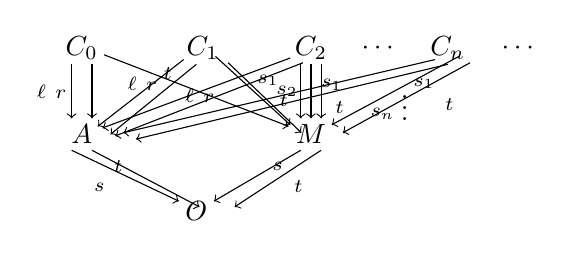
\begin{tikzpicture}[x=1.15em,y=1.15em]
  \node (C0) at (0,3.6)     {$C_{0}$};
  \node (C1) at (3.8,3.6)   {$C_{1}$};
  \node (C2) at (7.2,3.6)   {$C_{2}$};
  \node at (9.3,3.6)        {$\cdots$};
  \node (Cn) at (11.5,3.6)  {$C_{n}$};
  \node at (13.7,3.6)       {$\cdots$};
  \node (A) at (0,0.9)      {$A$};
  \node (M) at (7.2,0.9)    {$M$};
  \node (O) at (3.6,-1.5)   {$O$};
  \draw[->] (-0.32,3.1) -- (-0.32,1.4);
  \draw[->] (0.32,3.1)  -- (0.32,1.4);
  \node at (-0.95,2.25) {$\scriptstyle\ell\ r$};
  \draw[->] (3.2,3.25) -- (0.5,1.15);
  \draw[->] (3.6,3.1)  -- (0.9,0.9);
  \node at (1.9,2.5) {$\scriptstyle\ell\ r$};
  \draw[->] (6.55,3.3) -- (0.65,1.1);
  \draw[->] (6.95,3.15) -- (1.05,0.85);
  \node at (3.7,2.1) {$\scriptstyle\ell\ r$};
  \draw[->] (11.1,3.25) -- (1.3,0.95);
  \draw[->] (11.5,3.1)  -- (1.7,0.75);
  \draw[->] (0.7,3.4) -- (6.5,1.15);
  \node at (2.7,2.8) {$\scriptstyle t$};
  \draw[->] (4.2,3.35) -- (6.55,1.2);
  \node at (5.85,2.6) {$\scriptstyle s_{1}$};
  \draw[->] (4.6,3.15) -- (6.9,0.95);
  \node at (6.35,1.95) {$\scriptstyle t$};
  \draw[->] (6.88,3.1) -- (6.88,1.4);
  \draw[->] (7.2,3.1)  -- (7.2,1.4);
  \draw[->] (7.52,3.1) -- (7.52,1.4);
  \node at (6.45,2.25) {$\scriptstyle s_{2}$};
  \node at (7.85,2.45) {$\scriptstyle s_{1}$};
  \node at (8.1,1.75)  {$\scriptstyle t$};
  \draw[->] (11.85,3.35) -- (7.85,1.2);
  \node at (10.75,2.5) {$\scriptstyle s_{1}$};
  \node at (10.15,2.0) {$\scriptstyle\vdots$};
  \node at (9.45,1.55) {$\scriptstyle s_{n}$};
  \draw[->] (12.2,3.15) -- (8.2,0.95);
  \node at (11.55,1.85) {$\scriptstyle t$};
  \draw[->] (-0.32,0.4) -- (3.05,-1.2);
  \draw[->] (0.32,0.4)  -- (3.7,-1.38);
  \node at (1.15,-0.1) {$\scriptstyle t$};
  \node at (0.55,-0.75) {$\scriptstyle s$};
  \draw[->] (6.88,0.4) -- (4.15,-1.2);
  \draw[->] (7.52,0.4) -- (4.8,-1.38);
  \node at (6.15,-0.1) {$\scriptstyle s$};
  \node at (6.8,-0.75) {$\scriptstyle t$};
\end{tikzpicture}
\end{center}

每支箭头与每个模都拥有一个源对象与一个靶对象。每支 $n$ 元\trCell{}拥有一条左边
界箭头、一条右边界箭头、一个靶模以及 $n$ 个源模。此边界数据的源对象与靶对象
必须按由下列复合关系

\begin{equation*}
\begin{gathered}
s\cdot\ell = s\cdot s_{1} \qquad s\cdot r = t\cdot s_{n} \qquad t\cdot s_{k} = s\cdot s_{k+1},\quad 1\le k<n\\
t\cdot\ell = s\cdot t \qquad t\cdot r = t\cdot t
\end{gathered}
\end{equation*}

所指明的方式相容（于 $n\ge1$ 的情形\footnote{对零元\trCell，关系
$s\cdot\ell=s\cdot r$ 取代诸条涉及缺席源模的关系。}）。

另有两个种类 $I_{A}$ 与 $T$，分别参数化恒同竖直箭头与竖直箭头的复合，其复
合关系取自 1-范畴的签名：
\begin{equation*}
s\cdot i = t\cdot i \qquad s\cdot c = s\cdot\ell \qquad t\cdot c = t\cdot r \qquad t\cdot\ell = s\cdot r
\end{equation*}

每一类 $n$ 元\trCell{}都配备一个二元相等关系：
\begin{center}
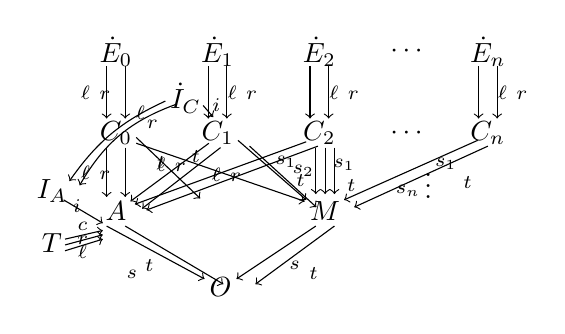
\begin{tikzpicture}[x=1.05em,y=1.05em]
  \node (E0) at (0,7.2)     {$\dot{E}_{0}$};
  \node (E1) at (3.5,7.2)   {$\dot{E}_{1}$};
  \node (E2) at (7.0,7.2)   {$\dot{E}_{2}$};
  \node at (10.0,7.2)       {$\cdots$};
  \node (En) at (12.8,7.2)  {$\dot{E}_{n}$};
  \node (IC) at (2.4,5.6)   {$\dot{I}_{C}$};
  \node (IA) at (-2.2,2.4)  {$I_{A}$};
  \node (T)  at (-2.2,0.6)  {$T$};
  \draw[->] (-0.32,6.7) -- (-0.32,4.9);
  \draw[->] (0.32,6.7)  -- (0.32,4.9);
  \node at (-0.7,5.8)  {$\scriptstyle\ell\ r$};
  \draw[->] (3.18,6.7) -- (3.18,4.9);
  \draw[->] (3.82,6.7) -- (3.82,4.9);
  \node at (4.35,5.8)  {$\scriptstyle\ell\ r$};
  \draw[->] (6.68,6.7) -- (6.68,4.9);
  \draw[->] (7.32,6.7) -- (7.32,4.9);
  \node at (7.85,5.8)  {$\scriptstyle\ell\ r$};
  \draw[->] (12.48,6.7) -- (12.48,4.9);
  \draw[->] (13.12,6.7) -- (13.12,4.9);
  \node at (13.65,5.8) {$\scriptstyle\ell\ r$};
  \draw[->] (3.0,5.35) -- (3.35,4.95);
  \node at (3.45,5.35) {$\scriptstyle i$};
  \draw[->] (1.7,5.5) to[bend right=15] (-1.6,2.75);
  \draw[->] (2.1,5.4) to[bend right=20] (-1.25,2.6);
  \node at (0.85,5.1) {$\scriptstyle\ell$};
  \node at (1.25,4.7) {$\scriptstyle r$};
  \node (C0) at (0,4.4)     {$C_{0}$};
  \node (C1) at (3.5,4.4)   {$C_{1}$};
  \node (C2) at (7.0,4.4)   {$C_{2}$};
  \node at (10.0,4.4)       {$\cdots$};
  \node (Cn) at (12.8,4.4)  {$C_{n}$};
  \draw[->] (0.7,4.25) -- (2.9,2.15);
  \node at (1.55,3.4) {$\scriptstyle t$};
  \draw[->] (-1.8,2.1) -- (-0.45,1.3);
  \node at (-1.35,1.9) {$\scriptstyle i$};
  \draw[->] (-1.75,0.75) -- (-0.45,1.05);
  \draw[->] (-1.75,0.55) -- (-0.45,0.9);
  \draw[->] (-1.75,0.35) -- (-0.45,0.75);
  \node at (-1.15,1.2) {$\scriptstyle c$};
  \node at (-1.15,0.72) {$\scriptstyle r$};
  \node at (-1.15,0.3) {$\scriptstyle \ell$};
  \draw[->] (-0.32,3.9) -- (-0.32,2.2);
  \draw[->] (0.32,3.9)  -- (0.32,2.2);
  \node at (-0.7,3.05) {$\scriptstyle\ell\ r$};
  \draw[->] (3.2,4.05) -- (0.5,2.05);
  \draw[->] (3.6,3.9)  -- (0.9,1.8);
  \node at (1.9,3.3) {$\scriptstyle\ell\ r$};
  \draw[->] (6.55,4.1) -- (0.65,1.95);
  \draw[->] (6.95,3.95) -- (1.05,1.75);
  \node at (3.8,2.95) {$\scriptstyle\ell\ r$};
  \draw[->] (0.7,4.05) -- (6.5,2.05);
  \node at (2.75,3.6) {$\scriptstyle t$};
  \draw[->] (4.2,4.15) -- (6.55,2.1);
  \node at (5.85,3.4) {$\scriptstyle s_{1}$};
  \draw[->] (4.6,3.95) -- (6.9,1.85);
  \node at (6.35,2.75) {$\scriptstyle t$};
  \draw[->] (6.88,3.9) -- (6.88,2.3);
  \draw[->] (7.2,3.9)  -- (7.2,2.3);
  \draw[->] (7.52,3.9) -- (7.52,2.3);
  \node at (6.45,3.1) {$\scriptstyle s_{2}$};
  \node at (7.85,3.3) {$\scriptstyle s_{1}$};
  \node at (8.1,2.6)  {$\scriptstyle t$};
  \draw[->] (12.45,4.15) -- (7.85,2.1);
  \node at (11.35,3.35) {$\scriptstyle s_{1}$};
  \node at (10.75,2.85) {$\scriptstyle\vdots$};
  \node at (10.05,2.4)  {$\scriptstyle s_{n}$};
  \draw[->] (12.8,3.95) -- (8.2,1.85);
  \node at (12.1,2.7) {$\scriptstyle t$};
  \node (A) at (0,1.7)    {$A$};
  \node (M) at (7.2,1.7)  {$M$};
  \node (O) at (3.6,-0.9) {$O$};
  \draw[->] (-0.32,1.2) -- (3.05,-0.62);
  \draw[->] (0.32,1.2)  -- (3.7,-0.8);
  \node at (1.15,-0.15) {$\scriptstyle t$};
  \node at (0.55,-0.45) {$\scriptstyle s$};
  \draw[->] (6.88,1.2) -- (4.15,-0.62);
  \draw[->] (7.52,1.2) -- (4.8,-0.8);
  \node at (6.15,-0.15) {$\scriptstyle s$};
  \node at (6.8,-0.45)  {$\scriptstyle t$};
\end{tikzpicture}
\end{center}

并满足一些等式，它们要求相等的\trCell{}必须具有相同的边界类型：
\begin{equation*}
\ell\cdot\ell = \ell\cdot r \qquad r\cdot\ell = r\cdot r \qquad t\cdot\ell = t\cdot r \qquad s_{k}\cdot\ell = s_{k}\cdot r
\end{equation*}

此外，在一个\trVirtualDoubleCategory{}中，每个模都拥有一支指定的恒同一元%
\trCell，其竖直源与靶为恒同箭头。关系符号 $\dot{I}_{C}$ 满足复合关系
\begin{equation*}
s\cdot i = t\cdot i \qquad \ell\cdot i = i\cdot\ell \qquad r\cdot i = i\cdot r
\end{equation*}
这些关系要求源模与靶模相重合，且左、右竖直箭头为恒同。

最后，对每一个分拆（partition）$n_{1}+\cdots+n_{k}=n$，都有一个 $(k+4)$ 元
关系符号 $\dot{T}_{n_{1},\ldots,n_{k}}$，其依赖关系如下图所示：
\begin{center}
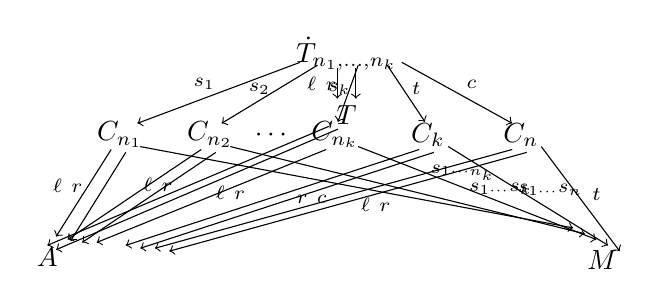
\begin{tikzpicture}[x=1.05em,y=1.05em]
  \node (Td) at (6.6,5.4) {$\dot{T}_{n_{1},\ldots,n_{k}}$};
  \node (Cn1) at (-1.2,2.6)  {$C_{n_{1}}$};
  \node (Cn2) at (1.9,2.6)   {$C_{n_{2}}$};
  \node at (4.0,2.6)          {$\cdots$};
  \node (Cnk) at (6.2,2.6)   {$C_{n_{k}}$};
  \node (Ck)  at (9.4,2.6)   {$C_{k}$};
  \node (Cn)  at (12.6,2.6)  {$C_{n}$};
  \draw[->] (5.0,5.1) -- (-0.6,3.0);
  \node at (1.7,4.35) {$\scriptstyle s_{1}$};
  \draw[->] (5.6,5.0) -- (2.3,3.0);
  \node at (3.6,4.2) {$\scriptstyle s_{2}$};
  \draw[->] (7.0,5.0) -- (6.3,3.05);
  \node at (6.35,4.2) {$\scriptstyle s_{k}$};
  \draw[->] (8.0,5.0) -- (9.3,3.05);
  \node at (9.0,4.2) {$\scriptstyle t$};
  \draw[->] (8.5,5.1) -- (12.3,3.0);
  \node at (10.9,4.35) {$\scriptstyle c$};
  \draw[->] (6.28,4.9) -- (6.28,3.85);
  \draw[->] (6.92,4.9) -- (6.92,3.85);
  \node at (5.75,4.35) {$\scriptstyle\ell\ r$};
  \node (T) at (6.6,3.3) {$T$};
  \draw[->] (-1.5,2.1) -- (-3.4,-0.9);
  \draw[->] (-1.0,2.0) -- (-2.9,-1.05);
  \node at (-3.0,0.85) {$\scriptstyle\ell\ r$};
  \draw[->] (1.6,2.1) -- (-3.0,-1.0);
  \draw[->] (2.1,2.0) -- (-2.5,-1.1);
  \node at (0.1,0.9) {$\scriptstyle\ell\ r$};
  \draw[->] (5.9,2.1) -- (-2.0,-1.1);
  \node at (2.6,0.6) {$\scriptstyle\ell\ r$};
  \draw[->] (9.1,2.1) -- (-1.0,-1.2);
  \draw[->] (9.6,2.0) -- (-0.5,-1.3);
  \node at (5.4,0.4) {$\scriptstyle r\ c$};
  \draw[->] (12.3,2.1) -- (0.0,-1.3);
  \draw[->] (12.8,2.0) -- (0.5,-1.4);
  \node at (7.6,0.2) {$\scriptstyle\ell\ r$};
  \draw[->] (-0.5,2.2) -- (14.4,-0.6);
  \draw[->] (2.6,2.2)  -- (14.8,-0.8);
  \node at (10.6,1.3) {$\scriptstyle s_{1\cdots n_{k}}$};
  \draw[->] (7.0,2.2) -- (15.2,-1.0);
  \node at (11.9,0.75) {$\scriptstyle s_{1\cdots}s_{k}$};
  \draw[->] (10.1,2.2) -- (15.6,-1.2);
  \node at (13.6,0.7) {$\scriptstyle s_{1\cdots}s_{n}$};
  \draw[->] (13.3,2.2) -- (16.0,-1.4);
  \node at (15.2,0.55) {$\scriptstyle t$};
  \draw[->] (6.0,2.9) -- (-3.7,-1.2);
  \draw[->] (6.3,2.8) -- (-3.4,-1.35);
  \node (A) at (-3.7,-1.6) {$A$};
  \node (M) at (15.4,-1.7) {$M$};
\end{tikzpicture}
\end{center}

并满足复合关系
\begin{equation*}
\begin{gathered}
s_{i}\cdot s_{j} = s_{n_{1}+\cdots+n_{j-1}+i}\cdot c \qquad
\ell\cdot\ell = \ell\cdot s_{1} \qquad
\ell\cdot r = r\cdot s_{k} \qquad
r\cdot s_{j} = \ell\cdot s_{j+1}\\
t\cdot s_{j} = s_{j}\cdot t \qquad
r\cdot\ell = \ell\cdot t \qquad
r\cdot r = r\cdot t\\
t\cdot t = t\cdot c \qquad
c\cdot\ell = \ell\cdot c \qquad
c\cdot r = r\cdot c
\end{gathered}
\end{equation*}

此处 $\dot{T}_{n_{1},\ldots,n_{k}}$ 是这样一个关系：它见证一支给定的 $n$ 元%
\trCell{}是 $k$ 支指定的源\trCell（元数（arity）分别为 $n_{1}$, \ldots, $n_{k}$）
复合入一支给定的靶 $k$ 元\trCell{}而成的复合。这样的复合还依赖于对竖直箭头的左、右交换
三角形的指定。

\begin{definition}\label{def:folds-signature-virtual-equipment}
\trVirtualEquipment{}的 FOLDS 签名 $\JVE$ 在\trVirtualDoubleCategory{}的
FOLDS 签名之上，添加两个额外的一元关系符号 $\dot{U}$ 与 $\dot{R}$，用以识别零
元单位\trModule{}与一元限制\trModule：
\end{definition}
\begin{center}
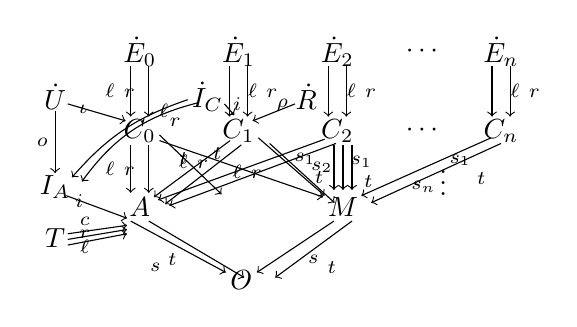
\begin{tikzpicture}[x=1.02em,y=1.02em]
  \node (U)  at (-3.0,5.6)  {$\dot{U}$};
  \node (E0) at (0,7.2)     {$\dot{E}_{0}$};
  \node (E1) at (3.5,7.2)   {$\dot{E}_{1}$};
  \node (E2) at (7.0,7.2)   {$\dot{E}_{2}$};
  \node at (10.0,7.2)       {$\cdots$};
  \node (En) at (12.8,7.2)  {$\dot{E}_{n}$};
  \node (IC) at (2.4,5.6)   {$\dot{I}_{C}$};
  \node (R)  at (5.9,5.6)   {$\dot{R}$};
  \node (IA) at (-3.0,2.4)  {$I_{A}$};
  \node (T)  at (-3.0,0.6)  {$T$};
  \draw[->] (-2.55,5.35) -- (-0.5,4.75);
  \node at (-2.0,5.15) {$\scriptstyle\iota$};
  \draw[->] (-3.0,5.1) -- (-3.0,2.9);
  \node at (-3.45,4.0) {$\scriptstyle o$};
  \draw[->] (5.5,5.35) -- (4.0,4.75);
  \node at (5.05,5.3) {$\scriptstyle\rho$};
  \draw[->] (-0.32,6.7) -- (-0.32,4.9);
  \draw[->] (0.32,6.7)  -- (0.32,4.9);
  \node at (-0.7,5.8)  {$\scriptstyle\ell\ r$};
  \draw[->] (3.18,6.7) -- (3.18,4.9);
  \draw[->] (3.82,6.7) -- (3.82,4.9);
  \node at (4.35,5.8)  {$\scriptstyle\ell\ r$};
  \draw[->] (6.68,6.7) -- (6.68,4.9);
  \draw[->] (7.32,6.7) -- (7.32,4.9);
  \node at (7.85,5.8)  {$\scriptstyle\ell\ r$};
  \draw[->] (12.48,6.7) -- (12.48,4.9);
  \draw[->] (13.12,6.7) -- (13.12,4.9);
  \node at (13.65,5.8) {$\scriptstyle\ell\ r$};
  \draw[->] (3.0,5.35) -- (3.35,4.95);
  \node at (3.45,5.35) {$\scriptstyle i$};
  \draw[->] (1.7,5.5) to[bend right=15] (-2.4,2.75);
  \draw[->] (2.1,5.4) to[bend right=20] (-2.05,2.6);
  \node at (0.85,5.1) {$\scriptstyle\ell$};
  \node at (1.25,4.7) {$\scriptstyle r$};
  \node (C0) at (0,4.4)     {$C_{0}$};
  \node (C1) at (3.5,4.4)   {$C_{1}$};
  \node (C2) at (7.0,4.4)   {$C_{2}$};
  \node at (10.0,4.4)       {$\cdots$};
  \node (Cn) at (12.8,4.4)  {$C_{n}$};
  \draw[->] (0.7,4.25) -- (2.9,2.15);
  \node at (1.55,3.4) {$\scriptstyle t$};
  \draw[->] (-2.6,2.1) -- (-0.45,1.3);
  \node at (-2.15,1.9) {$\scriptstyle i$};
  \draw[->] (-2.55,0.75) -- (-0.45,1.05);
  \draw[->] (-2.55,0.55) -- (-0.45,0.9);
  \draw[->] (-2.55,0.35) -- (-0.45,0.75);
  \node at (-1.95,1.2) {$\scriptstyle c$};
  \node at (-1.95,0.72) {$\scriptstyle r$};
  \node at (-1.95,0.3) {$\scriptstyle \ell$};
  \draw[->] (-0.32,3.9) -- (-0.32,2.2);
  \draw[->] (0.32,3.9)  -- (0.32,2.2);
  \node at (-0.7,3.05) {$\scriptstyle\ell\ r$};
  \draw[->] (3.2,4.05) -- (0.5,2.05);
  \draw[->] (3.6,3.9)  -- (0.9,1.8);
  \node at (1.9,3.3) {$\scriptstyle\ell\ r$};
  \draw[->] (6.55,4.1) -- (0.65,1.95);
  \draw[->] (6.95,3.95) -- (1.05,1.75);
  \node at (3.8,2.95) {$\scriptstyle\ell\ r$};
  \draw[->] (0.7,4.05) -- (6.5,2.05);
  \node at (2.75,3.6) {$\scriptstyle t$};
  \draw[->] (4.2,4.15) -- (6.55,2.1);
  \node at (5.85,3.4) {$\scriptstyle s_{1}$};
  \draw[->] (4.6,3.95) -- (6.9,1.85);
  \node at (6.35,2.75) {$\scriptstyle t$};
  \draw[->] (6.88,3.9) -- (6.88,2.3);
  \draw[->] (7.2,3.9)  -- (7.2,2.3);
  \draw[->] (7.52,3.9) -- (7.52,2.3);
  \node at (6.45,3.1) {$\scriptstyle s_{2}$};
  \node at (7.85,3.3) {$\scriptstyle s_{1}$};
  \node at (8.1,2.6)  {$\scriptstyle t$};
  \draw[->] (12.45,4.15) -- (7.85,2.1);
  \node at (11.35,3.35) {$\scriptstyle s_{1}$};
  \node at (10.75,2.85) {$\scriptstyle\vdots$};
  \node at (10.05,2.4)  {$\scriptstyle s_{n}$};
  \draw[->] (12.8,3.95) -- (8.2,1.85);
  \node at (12.1,2.7) {$\scriptstyle t$};
  \node (A) at (0,1.7)    {$A$};
  \node (M) at (7.2,1.7)  {$M$};
  \node (O) at (3.6,-0.9) {$O$};
  \draw[->] (-0.32,1.2) -- (3.05,-0.62);
  \draw[->] (0.32,1.2)  -- (3.7,-0.8);
  \node at (1.15,-0.15) {$\scriptstyle t$};
  \node at (0.55,-0.45) {$\scriptstyle s$};
  \draw[->] (6.88,1.2) -- (4.15,-0.62);
  \draw[->] (7.52,1.2) -- (4.8,-0.8);
  \node at (6.15,-0.15) {$\scriptstyle s$};
  \node at (6.8,-0.45)  {$\scriptstyle t$};
\end{tikzpicture}
\end{center}

单位模的左、右竖直箭头是同一对象上的恒同，这由如下复合关系表达：
\begin{equation*}
\ell\cdot\iota = i\cdot o = r\cdot\iota.
\end{equation*}

一元限制\trCell{}的边界不施加任何复合关系。这一数据便构成了 Cruttwell 与
Shulman 意义下\trVirtualEquipment{}的 FOLDS 签名。

任何\trVirtualEquipment{}都以一种朴素的（naïve）方式定义一个 $\JVE$-结构：取函子
$\JVE\to\mathcal{S}et$，令其把每个种类或关系符号送到其预期的解释（interpretation）。
\footnote{由于最令人感兴趣的虚拟装备都是大的，相应的 $\JVE$-结构也是大的。}
但正如 2-范畴的情形那样，对象 $I_{A}$ 与 $T$ 并非\trVirtualEquipment{}的
FOLDS 签名中的关系符号，故与这两个对象相关联的匹配映射无须
是\trMonomorphism。这使得我们有余地以一种更为「饱和的」方式把一
个\trVirtualEquipment{}转换为一个 $\JVE$-结构。事实上，与\cref{exa:pseudo-comma-2-category}和%
\cref{ex:naive-not-j-equivalent}相类比，为了证明我们想要的结果之一——%
\trVirtualEquipment{}间的一个\trBiequivalence{}给出（\cref{def:j-equivalent-in-context}意义下的）
一个 $\JVE$-等价——必须以这
种方式对与\trVirtualEquipment{}相关联的 $\JVE$-结构作「饱和化」（saturate）。
与\cref{exa:e-d-functors-2cat}中一样，也可以这样来定义与一个\trVirtualEquipment{}相关联的「饱
和的」$\JVE$-结构：定义一个从 $\JVE$ 到「\trVirtualEquipment{}及其保持结构的
函子」之\trCategory{}的相应反变函子；但在此情形，出现在指标图中的那些%
\trVirtualEquipment{}描述起来更为复杂，因此我们转而直接描述这一结构。

\begin{recall}\label{rec:vertical-two-category}
回顾第 8 章中的\cref{prop:vertical-two-category}：任何\trVirtualEquipment{}%
都包含一个%
\emph{竖直 2-范畴}（vertical 2-category），其对象是该\trVirtualEquipment{}的
对象，其箭头是竖直箭头，其 2-\trCell{}则是如下所示的那些一元\trCell：
\begin{rveq}\label{eq:vertical-2-category-unary-cell}
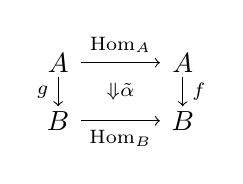
\begin{tikzpicture}[x=1.5em,y=1.5em]
  \node at (0,1.4) {$A$};
  \node at (3.0,1.4) {$A$};
  \draw[->] (0.55,1.4) -- node[above]{$\scriptstyle\mathrm{Hom}_{A}$} (2.45,1.4);
  \draw[->] (0,1.05) -- node[left]{$\scriptstyle g$} (0,0.35);
  \draw[->] (3.0,1.05) -- node[right]{$\scriptstyle f$} (3.0,0.35);
  \node at (1.5,0.7) {$\scriptstyle\Downarrow\tilde{\alpha}$};
  \node at (0,0) {$B$};
  \node at (3.0,0) {$B$};
  \draw[->] (0.55,0) -- node[below]{$\scriptstyle\mathrm{Hom}_{B}$} (2.45,0);
\end{tikzpicture}
\end{rveq}
其水平边界箭头由诸单位模给出。令人混淆的是，2-\trCell{}的「水平复合」由\trVirtualEquipment{}中一元\trCell{}%
的竖直复合来承载，而 2-\trCell{}的「竖直复合」则由第 8 章中的%
\cref{def:horizontal-composite-cells}所定义的水平复合运算来承载。特别地，当
竖直 2-范畴中的一元\trCell{}在 2-范畴中 2-\trCell{}的通常意义下可逆时——亦即
在\trVirtualEquipment{}中单位模之间的一元\trCell{}的水平复合运算意义下可逆时
——我们称其为「可逆的」；注意，竖直 2-范畴中一支可逆\trCell{}的竖直边界
1-\trCell{}无须在任何意义下可逆。

事实上，第 8 章中的\cref{def:horizontal-composite-cells}所描述的构造可作如
下推广。给定\trVirtualEquipment{}中的任意一支\trCell{}与一对竖直 2-范畴中的%
\trCell，如下所示
\begin{rveq}\label{eq:horizontal-composite-data}
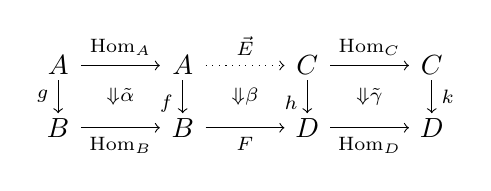
\begin{tikzpicture}[x=1.5em,y=1.5em]
  \node at (0,1.5)   {$A$};
  \node at (3.0,1.5) {$A$};
  \node at (6.0,1.5) {$C$};
  \node at (9.0,1.5) {$C$};
  \draw[->] (0.55,1.5) -- node[above]{$\scriptstyle\mathrm{Hom}_{A}$} (2.45,1.5);
  \draw[->,dotted] (3.55,1.5) -- node[above]{$\scriptstyle\vec{E}$} (5.45,1.5);
  \draw[->] (6.55,1.5) -- node[above]{$\scriptstyle\mathrm{Hom}_{C}$} (8.45,1.5);
  \draw[->] (0,1.15) -- node[left]{$\scriptstyle g$} (0,0.35);
  \node at (1.5,0.75) {$\scriptstyle\Downarrow\tilde{\alpha}$};
  \draw[->] (3.0,1.15) -- node[left,pos=0.7]{$\scriptstyle f$} (3.0,0.35);
  \node at (4.5,0.75) {$\scriptstyle\Downarrow\beta$};
  \draw[->] (6.0,1.15) -- node[left,pos=0.7]{$\scriptstyle h$} (6.0,0.35);
  \node at (7.5,0.75) {$\scriptstyle\Downarrow\tilde{\gamma}$};
  \draw[->] (9.0,1.15) -- node[right]{$\scriptstyle k$} (9.0,0.35);
  \node at (0,0)   {$B$};
  \node at (3.0,0) {$B$};
  \node at (6.0,0) {$D$};
  \node at (9.0,0) {$D$};
  \draw[->] (0.55,0) -- node[below]{$\scriptstyle\mathrm{Hom}_{B}$} (2.45,0);
  \draw[->] (3.55,0) -- node[below]{$\scriptstyle F$} (5.45,0);
  \draw[->] (6.55,0) -- node[below]{$\scriptstyle\mathrm{Hom}_{D}$} (8.45,0);
\end{tikzpicture}
\end{rveq}
存在唯一的一支「水平复合」\trCell，其边界为
\begin{rveq}\label{eq:horizontal-composite-cell}
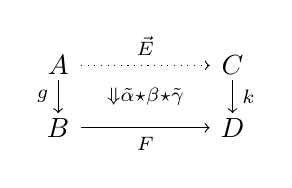
\begin{tikzpicture}[x=1.5em,y=1.5em]
  \node at (0,1.5) {$A$};
  \node at (4.2,1.5) {$C$};
  \draw[->,dotted] (0.55,1.5) -- node[above]{$\scriptstyle\vec{E}$} (3.65,1.5);
  \draw[->] (0,1.15) -- node[left]{$\scriptstyle g$} (0,0.35);
  \node at (2.1,0.75) {$\scriptstyle\Downarrow\tilde{\alpha}\star\beta\star\tilde{\gamma}$};
  \draw[->] (4.2,1.15) -- node[right]{$\scriptstyle k$} (4.2,0.35);
  \node at (0,0) {$B$};
  \node at (4.2,0) {$D$};
  \draw[->] (0.55,0) -- node[below]{$\scriptstyle F$} (3.65,0);
\end{tikzpicture}
\end{rveq}
并满足粘贴等式 \eqref{eq:horizontal-composite-pasting} 的类似物，后者是相对
于第 8 章中的\cref{lem:composites-with-units}的诸典范复合胞腔而定义的。在下
文中，我们将滥用记号，写出一个形如
\eqref{eq:horizontal-composite-data}的表达式来指称复合胞腔
\eqref{eq:horizontal-composite-cell}。

在\trInfinityCosmos{} $\mathcal{K}$ 中模的\trVirtualEquipment{}
$\Mod(\mathcal{K})$ 里，
这个竖直 2-范畴同构于\trHomotopyTwoCategory{} $\mathfrak{h}\mathcal{K}$。由
于我们打算在下述构造中应用于这一语境，故当从\trHomotopyTwoCategory{}借来的
记号更易读时，我们便借用之——例如，对竖直 2-范畴中右边界为 $f$、左边界为 $g$
的一支一元胞腔 \eqref{eq:vertical-2-category-unary-cell}，写作
$\alpha\colon f\Rightarrow g$。
\end{recall}

\begin{definition}\label{def:ve-structure-of-virtual-equipment}
对任何\trVirtualEquipment{} $\C$，都存在一个 $\JVE$-结构 $\Mof{\C}$，其中：
\begin{itemize}
\item 集合 $\Mof{\C}O$、$\Mof{\C}A$、$\Mof{\C}M$ 与诸 $\Mof{\C}C_{n}$（对每
个 $n\ge 0$）按其朴素解释分别取为 $\C$ 中对象、竖直箭头、水平\trModule{}与
$n$ 元\trCell{}的集合；
\item 诸二元关系 $\dot{E}_{n}$ 编码平行\trCell{}之间的相等；
\item 关系 $\dot{R}$ 编码全部\trCartesian{}一元\trCell，即满足刻画限制%
\trCell{}的那个\trUniversalProperty{}的\trCell；
\item 对任何 $i\colon \Mof{\C}A(X,X)$，$\Mof{\C}I_{A}\langle i\rangle$ 是竖
直 2-范畴中可逆\trCell{} $\alpha\colon \mathrm{id}_{X}\cong i$ 的集合；
\item 对任何 $i\colon \Mof{\C}A(X,X)$、$\alpha\colon \Mof{\C}I_{A}\langle i\rangle$、
$j\colon \Mof{\C}A(Y,Y)$、$\beta\colon \Mof{\C}I_{A}\langle j\rangle$、
$E\colon \Mof{\C}M(X,Y)$ 与 $\nu\colon \Mof{\C}C_{1}\langle i,j,E,E\rangle$：
若与模 $E$ 相关联的恒同\trCell{} $\mathrm{id}_{E}$ 等于水平复合\trCell
\begin{center}
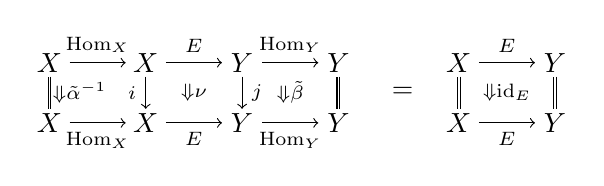
\begin{tikzpicture}[x=1.45em,y=1.45em]
  \node at (0,1.5)   {$X$};
  \node at (2.4,1.5) {$X$};
  \node at (4.8,1.5) {$Y$};
  \node at (7.2,1.5) {$Y$};
  \draw[->] (0.5,1.5) -- node[above]{$\scriptstyle\mathrm{Hom}_{X}$} (1.9,1.5);
  \draw[->] (2.9,1.5) -- node[above]{$\scriptstyle E$} (4.3,1.5);
  \draw[->] (5.3,1.5) -- node[above]{$\scriptstyle\mathrm{Hom}_{Y}$} (6.7,1.5);
  \draw[double,double distance=0.6pt] (0,1.15) -- (0,0.35);
  \node at (0.75,0.75) {$\scriptstyle\Downarrow\tilde{\alpha}^{-1}$};
  \draw[->] (2.4,1.15) -- node[left]{$\scriptstyle i$} (2.4,0.35);
  \node at (3.6,0.75) {$\scriptstyle\Downarrow\nu$};
  \draw[->] (4.8,1.15) -- node[right]{$\scriptstyle j$} (4.8,0.35);
  \node at (6.0,0.75) {$\scriptstyle\Downarrow\tilde{\beta}$};
  \draw[double,double distance=0.6pt] (7.2,1.15) -- (7.2,0.35);
  \node at (0,0)   {$X$};
  \node at (2.4,0) {$X$};
  \node at (4.8,0) {$Y$};
  \node at (7.2,0) {$Y$};
  \draw[->] (0.5,0) -- node[below]{$\scriptstyle\mathrm{Hom}_{X}$} (1.9,0);
  \draw[->] (2.9,0) -- node[below]{$\scriptstyle E$} (4.3,0);
  \draw[->] (5.3,0) -- node[below]{$\scriptstyle\mathrm{Hom}_{Y}$} (6.7,0);
  \node at (8.8,0.75) {$=$};
  \begin{scope}[shift={(10.2,0)}]
  \node at (0,1.5) {$X$};
  \node at (2.4,1.5) {$Y$};
  \draw[->] (0.5,1.5) -- node[above]{$\scriptstyle E$} (1.9,1.5);
  \draw[double,double distance=0.6pt] (0,1.15) -- (0,0.35);
  \node at (1.2,0.75) {$\scriptstyle\Downarrow\mathrm{id}_{E}$};
  \draw[double,double distance=0.6pt] (2.4,1.15) -- (2.4,0.35);
  \node at (0,0) {$X$};
  \node at (2.4,0) {$Y$};
  \draw[->] (0.5,0) -- node[below]{$\scriptstyle E$} (1.9,0);
  \end{scope}
\end{tikzpicture}
\end{center}
则 $\Mof{\C}\dot{I}_{C}\langle\nu\rangle$ 为单点集，否则为空；
\item 对 $i\colon \Mof{\C}A(X,X)$、$\alpha\colon \Mof{\C}I_{A}\langle i\rangle$、
$H\colon \Mof{\C}M(X,X)$ 与 $\theta\colon \Mof{\C}C_{0}\langle i,i,H\rangle$：
若零元复合\trCell
\begin{center}
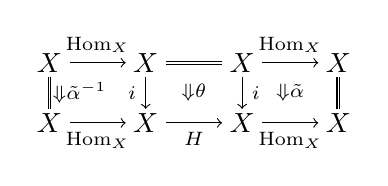
\begin{tikzpicture}[x=1.45em,y=1.45em]
  \node at (0,1.5)   {$X$};
  \node at (2.4,1.5) {$X$};
  \node at (4.8,1.5) {$X$};
  \node at (7.2,1.5) {$X$};
  \draw[->] (0.5,1.5) -- node[above]{$\scriptstyle\mathrm{Hom}_{X}$} (1.9,1.5);
  \draw[double,double distance=0.6pt] (2.9,1.5) -- (4.3,1.5);
  \draw[->] (5.3,1.5) -- node[above]{$\scriptstyle\mathrm{Hom}_{X}$} (6.7,1.5);
  \draw[double,double distance=0.6pt] (0,1.15) -- (0,0.35);
  \node at (0.75,0.75) {$\scriptstyle\Downarrow\tilde{\alpha}^{-1}$};
  \draw[->] (2.4,1.15) -- node[left]{$\scriptstyle i$} (2.4,0.35);
  \node at (3.6,0.75) {$\scriptstyle\Downarrow\theta$};
  \draw[->] (4.8,1.15) -- node[right]{$\scriptstyle i$} (4.8,0.35);
  \node at (6.0,0.75) {$\scriptstyle\Downarrow\tilde{\alpha}$};
  \draw[double,double distance=0.6pt] (7.2,1.15) -- (7.2,0.35);
  \node at (0,0)   {$X$};
  \node at (2.4,0) {$X$};
  \node at (4.8,0) {$X$};
  \node at (7.2,0) {$X$};
  \draw[->] (0.5,0) -- node[below]{$\scriptstyle\mathrm{Hom}_{X}$} (1.9,0);
  \draw[->] (2.9,0) -- node[below]{$\scriptstyle H$} (4.3,0);
  \draw[->] (5.3,0) -- node[below]{$\scriptstyle\mathrm{Hom}_{X}$} (6.7,0);
\end{tikzpicture}
\end{center}
是余笛卡尔的，则 $\Mof{\C}\dot{U}\langle i,\theta\rangle$ 为单点集，否则为空；
\item 对任何 $f\colon \Mof{\C}A(X,Y)$、$g\colon \Mof{\C}A(Y,Z)$ 与
$h\colon \Mof{\C}A(X,Z)$，$\Mof{\C}T\langle f,g,h\rangle$ 是竖直 2-范畴中可
逆\trCell{} $\gamma\colon gf\cong h$ 的集合；
\item 对任何 $n_{1}+\cdots+n_{k}=n$，给定诸\trCell
\begin{center}
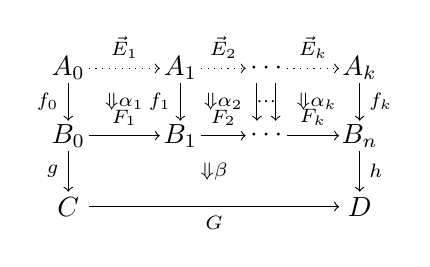
\begin{tikzpicture}[x=1.35em,y=1.35em]
  \node (A0) at (0,3.0)    {$A_{0}$};
  \node (A1) at (3.0,3.0)  {$A_{1}$};
  \node at (5.3,3.0)       {$\cdots$};
  \node (Ak) at (7.8,3.0)  {$A_{k}$};
  \draw[->,dotted] (0.55,3.0) -- node[above]{$\scriptstyle\vec{E}_{1}$} (2.45,3.0);
  \draw[->,dotted] (3.55,3.0) -- node[above]{$\scriptstyle\vec{E}_{2}$} (4.75,3.0);
  \draw[->,dotted] (5.85,3.0) -- node[above]{$\scriptstyle\vec{E}_{k}$} (7.25,3.0);
  \draw[->] (0,2.6) -- node[left]{$\scriptstyle f_{0}$} (0,1.6);
  \draw[->] (3.0,2.6) -- node[left]{$\scriptstyle f_{1}$} (3.0,1.6);
  \draw[->] (5.05,2.6) -- (5.05,1.6);
  \draw[->] (5.55,2.6) -- (5.55,1.6);
  \node at (5.3,2.1) {$\scriptstyle\cdots$};
  \draw[->] (7.8,2.6) -- node[right]{$\scriptstyle f_{k}$} (7.8,1.6);
  \node at (1.5,2.1)  {$\scriptstyle\Downarrow\alpha_{1}$};
  \node at (4.15,2.1) {$\scriptstyle\Downarrow\alpha_{2}$};
  \node at (6.65,2.1) {$\scriptstyle\Downarrow\alpha_{k}$};
  \node (B0) at (0,1.2)   {$B_{0}$};
  \node (B1) at (3.0,1.2) {$B_{1}$};
  \node at (5.3,1.2)      {$\cdots$};
  \node (Bn) at (7.8,1.2) {$B_{n}$};
  \draw[->] (0.55,1.2) -- node[above]{$\scriptstyle F_{1}$} (2.45,1.2);
  \draw[->] (3.55,1.2) -- node[above]{$\scriptstyle F_{2}$} (4.75,1.2);
  \draw[->] (5.85,1.2) -- node[above]{$\scriptstyle F_{k}$} (7.25,1.2);
  \draw[->] (0,0.8) -- node[left]{$\scriptstyle g$} (0,-0.3);
  \draw[->] (7.8,0.8) -- node[right]{$\scriptstyle h$} (7.8,-0.3);
  \node at (3.9,0.25) {$\scriptstyle\Downarrow\beta$};
  \node (C) at (0,-0.7)   {$C$};
  \node (D) at (7.8,-0.7) {$D$};
  \draw[->] (0.55,-0.7) -- node[below]{$\scriptstyle G$} (7.25,-0.7);
\end{tikzpicture}\\[1.2em]
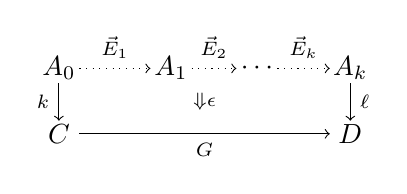
\begin{tikzpicture}[x=1.35em,y=1.35em]
  \node (A0) at (0,1.6)    {$A_{0}$};
  \node (A1) at (3.0,1.6)  {$A_{1}$};
  \node at (5.3,1.6)       {$\cdots$};
  \node (Ak) at (7.8,1.6)  {$A_{k}$};
  \draw[->,dotted] (0.55,1.6) -- node[above]{$\scriptstyle\vec{E}_{1}$} (2.45,1.6);
  \draw[->,dotted] (3.55,1.6) -- node[above]{$\scriptstyle\vec{E}_{2}$} (4.75,1.6);
  \draw[->,dotted] (5.85,1.6) -- node[above]{$\scriptstyle\vec{E}_{k}$} (7.25,1.6);
  \draw[->] (0,1.2) -- node[left]{$\scriptstyle k$} (0,0.2);
  \draw[->] (7.8,1.2) -- node[right]{$\scriptstyle\ell$} (7.8,0.2);
  \node at (3.9,0.7) {$\scriptstyle\Downarrow\epsilon$};
  \node (C) at (0,-0.15)   {$C$};
  \node (D) at (7.8,-0.15) {$D$};
  \draw[->] (0.55,-0.15) -- node[below]{$\scriptstyle G$} (7.25,-0.15);
\end{tikzpicture}
\end{center}
与任意一对同构 $\gamma\colon T\langle f_{0},g,k\rangle$ 与
$\delta\colon T\langle f_{k},h,\ell\rangle$：若 $\epsilon$ 等于复合
\begin{center}
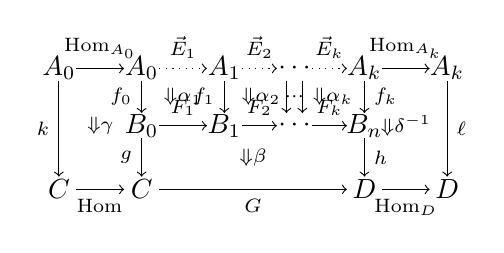
\begin{tikzpicture}[x=1.15em,y=1.15em]
  \node (A0a) at (0,3.0)    {$A_{0}$};
  \node (A0b) at (2.6,3.0)  {$A_{0}$};
  \node (A1)  at (5.2,3.0)  {$A_{1}$};
  \node at (7.4,3.0)        {$\cdots$};
  \node (Ak1) at (9.6,3.0)  {$A_{k}$};
  \node (Ak2) at (12.2,3.0) {$A_{k}$};
  \draw[->] (0.55,3.0) -- node[above]{$\scriptstyle\mathrm{Hom}_{A_{0}}$} (2.05,3.0);
  \draw[->,dotted] (3.15,3.0) -- node[above]{$\scriptstyle\vec{E}_{1}$} (4.65,3.0);
  \draw[->,dotted] (5.75,3.0) -- node[above]{$\scriptstyle\vec{E}_{2}$} (6.85,3.0);
  \draw[->,dotted] (7.95,3.0) -- node[above]{$\scriptstyle\vec{E}_{k}$} (9.05,3.0);
  \draw[->] (10.15,3.0) -- node[above]{$\scriptstyle\mathrm{Hom}_{A_{k}}$} (11.65,3.0);
  \draw[->] (0,2.6) -- node[left]{$\scriptstyle k$} (0,-0.4);
  \draw[->] (12.2,2.6) -- node[right]{$\scriptstyle\ell$} (12.2,-0.4);
  \draw[->] (2.6,2.6) -- node[left]{$\scriptstyle f_{0}$} (2.6,1.6);
  \draw[->] (5.2,2.6) -- node[left]{$\scriptstyle f_{1}$} (5.2,1.6);
  \draw[->] (7.15,2.6) -- (7.15,1.6);
  \draw[->] (7.65,2.6) -- (7.65,1.6);
  \node at (7.4,2.1) {$\scriptstyle\cdots$};
  \draw[->] (9.6,2.6) -- node[right]{$\scriptstyle f_{k}$} (9.6,1.6);
  \node at (3.9,2.1)  {$\scriptstyle\Downarrow\alpha_{1}$};
  \node at (6.35,2.1) {$\scriptstyle\Downarrow\alpha_{2}$};
  \node at (8.6,2.1)  {$\scriptstyle\Downarrow\alpha_{k}$};
  \node at (1.3,1.2)  {$\scriptstyle\Downarrow\gamma$};
  \node at (10.9,1.2) {$\scriptstyle\Downarrow\delta^{-1}$};
  \node (B0) at (2.6,1.2)  {$B_{0}$};
  \node (B1) at (5.2,1.2)  {$B_{1}$};
  \node at (7.4,1.2)       {$\cdots$};
  \node (Bn) at (9.6,1.2)  {$B_{n}$};
  \draw[->] (3.15,1.2) -- node[above]{$\scriptstyle F_{1}$} (4.65,1.2);
  \draw[->] (5.75,1.2) -- node[above]{$\scriptstyle F_{2}$} (6.85,1.2);
  \draw[->] (7.95,1.2) -- node[above]{$\scriptstyle F_{k}$} (9.05,1.2);
  \draw[->] (2.6,0.8) -- node[left]{$\scriptstyle g$} (2.6,-0.4);
  \draw[->] (9.6,0.8) -- node[right]{$\scriptstyle h$} (9.6,-0.4);
  \node at (6.1,0.2) {$\scriptstyle\Downarrow\beta$};
  \node (C0) at (0,-0.8)    {$C$};
  \node (C1) at (2.6,-0.8)  {$C$};
  \node (D1) at (9.6,-0.8)  {$D$};
  \node (D2) at (12.2,-0.8) {$D$};
  \draw[->] (0.55,-0.8) -- node[below]{$\scriptstyle\mathrm{Hom}_{\C}$} (2.05,-0.8);
  \draw[->] (3.15,-0.8) -- node[below]{$\scriptstyle G$} (9.05,-0.8);
  \draw[->] (10.15,-0.8) -- node[below]{$\scriptstyle\mathrm{Hom}_{\mathbb{D}}$} (11.65,-0.8);
\end{tikzpicture}
\end{center}
则集合 $\Mof{\C}\dot{T}_{n_{1},\ldots,n_{k}}\langle\alpha_{1},\ldots,\alpha_{k},\beta,\epsilon,\gamma,\delta\rangle$
为单点集，否则为空。
\end{itemize}
\end{definition}

我们记 $\Mof{\mathcal{K}}\colon \JVE\to\mathcal{S}et$ 为把%
\cref{def:ve-structure-of-virtual-equipment}的构造
施用于模的\trVirtualEquipment{} $\Mod(\mathcal{K})$ 而得的 $\JVE$-结构。

\begin{remark}\label{rem:natural-transformation-of-structures}
回顾：\trVirtualEquipment{}间的一个\trFunctor{} $F\colon\C\to\mathbb{D}$ 是
一个保持全部结构——包括单位\trCell{}与限制\trCell——的%
\trVirtualDoubleCategory{}间的映射。于是，施用 $F$ 便直接
给出了相应诸 $\JVE$-结构之间一个\trNaturalTransformation{}
$F\colon\Mof{\C}\to\Mof{\mathbb{D}}$ 的诸分量。依据%
\cref{prop:cosmological-functor-induces-ve-functor}，一个\trCosmologicalFunctor{}
$F\colon\mathcal{K}\to\mathcal{L}$ 诱导\trVirtualEquipment{}间的一个\trFunctor{}
$F\colon\Mod(\mathcal{K})\to\Mod(\mathcal{L})$，从而诱导 $\JVE$-结构之间的一
个\trNaturalTransformation{} $F\colon\Mof{\mathcal{K}}\to\Mof{\mathcal{L}}$。
\end{remark}

\begin{proposition}\label{prop:biequivalence-gives-ve-equivalence}
考虑由一个\trCosmologicalFunctor{} $F\colon\mathcal{K}\to\mathcal{L}$ 相连的
一对\trInfinityCosmos。
\begin{enumerate}[label=(\roman*)]
\item 若 $F\colon\mathcal{K}\to\mathcal{L}$ 是一个\trCosmologicalBiequivalence，
则在相应的诸 $\JVE$-结构之间存在一对逐纤维满射：
\begin{center}
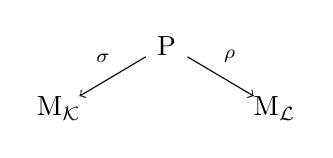
\begin{tikzpicture}[x=1.5em,y=1.5em]
  \node (P) at (0,1.5)  {$\mathrm{P}$};
  \node (K) at (-2.6,0) {$\Mof{\mathcal{K}}$};
  \node (L) at (2.6,0)  {$\Mof{\mathcal{L}}$};
  \draw[->] (-0.5,1.25) -- node[above left,pos=0.4]{$\scriptstyle\sigma$} (-2.1,0.3);
  \draw[->] (0.5,1.25) -- node[above right,pos=0.4]{$\scriptstyle\rho$} (2.1,0.3);
\end{tikzpicture}
\end{center}
\item 此外，若 $\JVE$-结构之间的受诱导映射保持一个上下文 $\Gamma$
的给定解释
\begin{center}
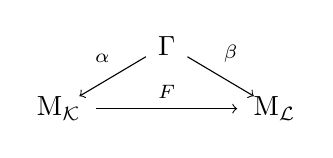
\begin{tikzpicture}[x=1.5em,y=1.5em]
  \node (G) at (0,1.5)  {$\Gamma$};
  \node (K) at (-2.6,0) {$\Mof{\mathcal{K}}$};
  \node (L) at (2.6,0)  {$\Mof{\mathcal{L}}$};
  \draw[->] (-0.5,1.25) -- node[above left,pos=0.4]{$\scriptstyle\alpha$} (-2.1,0.3);
  \draw[->] (0.5,1.25) -- node[above right,pos=0.4]{$\scriptstyle\beta$} (2.1,0.3);
  \draw[->] (-1.7,0) -- node[above]{$\scriptstyle F$} (1.7,0);
\end{tikzpicture}
\end{center}
则 (i) 中构造的诸逐纤维满射给出上下文 $\Gamma$ 中的一个 $\JVE$-等价：
\begin{center}
\begin{tikzpicture}[x=1.5em,y=1.5em]
  \node (G) at (0,2.6)  {$\Gamma$};
  \node (K) at (-2.6,1.3) {$\Mof{\mathcal{K}}$};
  \node (L) at (2.6,1.3)  {$\Mof{\mathcal{L}}$};
  \node (P) at (0,0)    {$\mathrm{P}$};
  \draw[->] (-0.5,2.35) -- node[above left,pos=0.4]{$\scriptstyle\alpha$} (-2.1,1.6);
  \draw[->] (0.5,2.35) -- node[above right,pos=0.4]{$\scriptstyle\beta$} (2.1,1.6);
  \draw[->] (0,2.2) -- node[right]{$\scriptstyle\gamma$} (0,0.45);
  \draw[->] (-0.5,0.25) -- node[below left,pos=0.4]{$\scriptstyle\sigma$} (-2.1,1.0);
  \draw[->] (0.5,0.25) -- node[below right,pos=0.4]{$\scriptstyle\rho$} (2.1,1.0);
\end{tikzpicture}
\end{center}
\end{enumerate}
\end{proposition}

\begin{proof}
我们采用与\cref{exa:jcat-equivalence-iso-comma}和\cref{exa:pseudo-comma-2-category}中相同的策略，构造一个结构，称之为与%
\trVirtualEquipment{}间的\trFunctor{}
$F\colon\Mod(\mathcal{K})\to\Mod(\mathcal{L})$ 相关联的%
\emph{伪逗号\trVirtualEquipment}（pseudo-comma virtual equipment）$\mathbb{P}$。\footnote{%
伪逗号\trVirtualEquipment{}对\trVirtualEquipment{}之间的任何\trFunctor（或更
一般地，\trFunctor{}的%
\trCospan）都可用完全相同的方式定义；但在记号得以简化之处，我们亦将此种说法
用于\trInfinityCosmos{}中的结构及其\trHomotopyTwoCategory。}
$\JVE$-结构 $\mathrm{P}$ 随之定义为 $\Mof{\mathbb{P}}$，而 $\sigma$ 与 $\rho$
则是显然的投射。然后我们论证：在 $F$ 是\trVirtualEquipment{}间的一个%
\trBiequivalence{}这一假设下，这两个映射是逐纤维满的。

与 $F\colon\Mod(\mathcal{K})\to\Mod(\mathcal{L})$ 相关联的\textbf{伪逗号%
\trVirtualEquipment} $\mathbb{P}$ 拥有：
\begin{itemize}
\item 对象由三元组 $(A\in\mathcal{K},\,A'\in\mathcal{L},\,a\colon FA\Rightarrow A'\in\mathcal{L})$
给出，其中 $a$ 是一个\trEquivalence；
\item 竖直箭头 $(A,A',a)\to(B,B',b)$ 由如下形状的三元组给出
\[
\left(\;
\begin{tikzpicture}[x=1.35em,y=1.35em]
  \node at (0,1.5)    {$A$};
  \node at (3.0,1.5)  {$A'$};
  \node at (6.2,1.5)  {$FA$};
  \node at (9.4,1.5)  {$A'$};
  \draw[->] (6.85,1.5) -- node[above]{$\scriptstyle a$} (8.75,1.5);
  \draw[->] (0,1.15) -- node[left]{$\scriptstyle f$} (0,0.35);
  \node at (0.8,0.4) {$\scriptstyle\in\mathcal{K}$};
  \draw[->] (3.0,1.15) -- node[left]{$\scriptstyle f'$} (3.0,0.35);
  \node at (3.9,0.4) {$\scriptstyle\in\mathcal{L}$};
  \draw[->] (6.2,1.15) -- node[left]{$\scriptstyle Ff$} (6.2,0.35);
  \node at (7.55,0.75) {$\scriptstyle\cong\alpha$};
  \draw[->] (9.4,1.15) -- node[right]{$\scriptstyle f'$} (9.4,0.35);
  \node at (10.6,0.75) {$\scriptstyle\in\mathfrak{h}\mathcal{L}$};
  \node at (0,0)    {$B$};
  \node at (3.0,0)  {$B'$};
  \node at (6.2,0)  {$FB$};
  \node at (9.4,0)  {$B'$};
  \draw[->] (6.85,0) -- node[below]{$\scriptstyle b$} (8.75,0);
\end{tikzpicture}
\;\right)
\]
\item 模 $(A,A',a)\longmapsto(B,B',b)$ 由如下形状的三元组给出
\[
\left(\;
\begin{tikzpicture}[x=1.35em,y=1.35em]
  \node at (0,1.4)   {$A$};
  \node at (2.6,1.4) {$B$};
  \draw[->] (0.5,1.4) -- node[above]{$\scriptstyle E$} (2.1,1.4);
  \node at (3.8,1.4) {$\scriptstyle\in\mathcal{K}$};
  \node at (5.2,1.4)  {$A'$};
  \node at (7.8,1.4)  {$B'$};
  \draw[->] (5.7,1.4) -- node[above]{$\scriptstyle E'$} (7.3,1.4);
  \node at (9.0,1.4) {$\scriptstyle\in\mathcal{L}$};
  \node at (11.4,2.1) {$FA$};
  \node at (14.4,2.1) {$FB$};
  \draw[->] (12.05,2.1) -- node[above]{$\scriptstyle FE$} (13.75,2.1);
  \draw[->] (11.4,1.75) -- node[left]{$\scriptstyle a$} (11.4,0.95);
  \node at (12.7,1.35) {$\scriptstyle\Downarrow\epsilon$};
  \draw[->] (14.4,1.75) -- node[right]{$\scriptstyle b$} (14.4,0.95);
  \node at (11.4,0.6)  {$A'$};
  \node at (14.4,0.6)  {$B'$};
  \draw[->] (12.05,0.6) -- node[below]{$\scriptstyle E'$} (13.75,0.6);
  \node at (15.9,1.35) {$\scriptstyle\in\Mod(\mathcal{L})$};
\end{tikzpicture}
\;\right)
\]
其中 $\epsilon$ 是一支\trCartesian\trCell；
\item $n$ 元\trCell{}由一对 $n$ 元\trCell——$\mathcal{K}$ 中的 $\mu$ 与
$\mathcal{L}$ 中的 $\nu$——给出，使得由其边界数据形成的复合\trCell{}相等：
\begin{center}
\begin{tikzpicture}[x=1.15em,y=1.15em]
  \node at (0,2.6)     {$FA_{0}$};
  \node at (3.0,2.6)   {$FA_{0}$};
  \node at (6.0,2.6)   {$FA_{1}$};
  \node at (9.0,2.6)   {$FA_{2}$};
  \node at (11.0,2.6)  {$\cdots$};
  \node at (13.0,2.6)  {$FA_{n}$};
  \draw[->] (0.75,2.6) -- node[above]{$\scriptstyle F\mathrm{Hom}_{A_{0}}$} (2.25,2.6);
  \draw[->] (3.75,2.6) -- node[above]{$\scriptstyle FE_{1}$} (5.25,2.6);
  \draw[->] (6.75,2.6) -- node[above]{$\scriptstyle FE_{2}$} (8.25,2.6);
  \draw[->] (11.55,2.6) -- node[above]{$\scriptstyle FE_{n}$} (12.3,2.6);
  \draw[->] (0,2.2) -- node[left]{$\scriptstyle a_{0}$} (0,1.3);
  \draw[->] (3.0,2.2) -- node[left]{$\scriptstyle Ff$} (3.0,1.3);
  \node at (7.5,1.75) {$\scriptstyle\Downarrow F\mu$};
  \draw[->] (13.0,2.2) -- node[right]{$\scriptstyle Fg$} (13.0,1.3);
  \node at (0,0.9)  {$A'_{0}$};
  \node at (3.0,0.9){$FB$};
  \node at (9.6,0.9){$FC$};
  \draw[->] (0,0.55) -- node[left]{$\scriptstyle f'$} (0,-0.35);
  \node at (1.0,0.7) {$\scriptstyle\Downarrow\tilde{\alpha}$};
  \node at (3.0,0.55) {$\scriptstyle b$};
  \draw[->] (3.55,0.9) -- node[below]{$\scriptstyle FG$} (8.9,0.9);
  \draw[->] (9.6,0.55) -- node[right]{$\scriptstyle c$} (9.6,-0.35);
  \node at (4.1,0.2) {$\scriptstyle\Downarrow\epsilon$};
  \node at (0,-0.7)  {$B'$};
  \node at (3.0,-0.7){$B'$};
  \node at (9.6,-0.7){$C'$};
  \draw[->] (0.5,-0.7) -- node[below]{$\scriptstyle\mathrm{Hom}_{B'}$} (2.25,-0.7);
  \draw[->] (3.75,-0.7) -- node[below]{$\scriptstyle G'$} (8.9,-0.7);
  \node at (11.4,0.9) {$=$};
  \begin{scope}[shift={(13.6,0)}]
  \node at (0,2.6)     {$FA_{0}$};
  \node at (3.0,2.6)   {$FA_{1}$};
  \node at (6.0,2.6)   {$FA_{2}$};
  \node at (8.0,2.6)   {$\cdots$};
  \node at (10.0,2.6)  {$FA_{n}$};
  \node at (13.0,2.6)  {$FA_{n}$};
  \draw[->] (0.75,2.6) -- node[above]{$\scriptstyle FE_{1}$} (2.25,2.6);
  \draw[->] (3.75,2.6) -- node[above]{$\scriptstyle FE_{2}$} (5.25,2.6);
  \draw[->] (6.55,2.6) -- node[above]{$\scriptstyle FE_{n}$} (9.3,2.6);
  \draw[->] (10.75,2.6) -- node[above]{$\scriptstyle F\mathrm{Hom}_{A_{n}}$} (12.25,2.6);
  \draw[->] (0,2.2) -- node[left]{$\scriptstyle a_{0}$} (0,1.3);
  \node at (1.5,1.75) {$\scriptstyle\Downarrow\epsilon$};
  \draw[->] (3.0,2.2) -- node[left]{$\scriptstyle a_{1}$} (3.0,1.3);
  \node at (4.5,1.75) {$\scriptstyle\Downarrow\epsilon$};
  \node at (6.5,1.75) {$\scriptstyle\cdots$};
  \node at (8.0,1.75) {$\scriptstyle\Downarrow\epsilon$};
  \draw[->] (10.0,2.2) -- node[left]{$\scriptstyle a_{n}$} (10.0,1.3);
  \draw[->] (13.0,2.2) -- node[right]{$\scriptstyle Fg$} (13.0,1.3);
  \node at (0,0.9)   {$A'_{0}$};
  \node at (3.0,0.9) {$A'_{1}$};
  \node at (6.0,0.9) {$A'_{2}$};
  \node at (8.0,0.9) {$\cdots$};
  \node at (10.0,0.9){$A'_{n}$};
  \node at (13.0,0.9){$FC$};
  \draw[->] (0.75,0.9) -- node[above]{$\scriptstyle E'_{1}$} (2.25,0.9);
  \draw[->] (3.75,0.9) -- node[above]{$\scriptstyle E'_{2}$} (5.25,0.9);
  \draw[->] (6.55,0.9) -- node[above]{$\scriptstyle E'_{n}$} (9.3,0.9);
  \node at (11.5,1.3) {$\scriptstyle\Downarrow\tilde{\beta}$};
  \draw[->] (0,0.55) -- node[left]{$\scriptstyle f'$} (0,-0.35);
  \node at (4.5,0.2) {$\scriptstyle\Downarrow\nu$};
  \draw[->] (10.0,0.55) -- node[left]{$\scriptstyle g'$} (10.0,-0.35);
  \draw[->] (13.0,0.55) -- node[right]{$\scriptstyle c$} (13.0,-0.35);
  \node at (0,-0.7)  {$B'$};
  \node at (10.0,-0.7){$C'$};
  \node at (13.0,-0.7){$C'$};
  \draw[->] (0.75,-0.7) -- node[below]{$\scriptstyle G'$} (9.3,-0.7);
  \draw[->] (10.75,-0.7) -- node[below]{$\scriptstyle\mathrm{Hom}_{C'}$} (12.25,-0.7);
  \end{scope}
\end{tikzpicture}
\end{center}
\end{itemize}

我们来论证 $\mathbb{P}$ 是一个\trVirtualDoubleCategory。注意其对象与竖直箭头
构成一个\trCategory：事实上，它正是\cref{exa:pseudo-comma-2-category}中\trTwoFunctor
$F\colon\mathfrak{h}\mathcal{K}\to\mathfrak{h}\mathcal{L}$ 的伪逗号 2-范畴的
底 1-范畴。每个模 $(E,E',\epsilon)\colon(A,A',a)\longmapsto(B,B',b)$ 都拥有
一支恒同\trCell，其分量为 $\mathcal{K}$ 中的恒同\trCell{} $\mathrm{id}_{E}$ 与
$\mathcal{L}$ 中的恒同\trCell{} $\mathrm{id}_{E'}$。诸\trCell{}的复合承袭自
$\Mod(\mathcal{K})$ 与 $\Mod(\mathcal{L})$，不过所需的、以这种方式定义的复合%
\trCell{}之间的粘贴等式，我们留给读者画一张非常大的图来验证。这使得
$\mathbb{P}$ 成为一个\trVirtualDoubleCategory。

事实上，$\mathbb{P}$ 是一个\trVirtualEquipment。每个对象 $(A,A',a)$ 容许
形如 $(\mathrm{Hom}_{A},\mathrm{Hom}_{A'},\mathrm{Hom}_{a})$ 的一个单位模，
并配备一支零元%
\trCocartesian\trCell
\begin{center}
\begin{tikzpicture}[x=1.3em,y=1.3em]
  \node at (0,1.9)   {$(A,A',a)$};
  \node at (3.6,1.9) {$(A,A',a)$};
  \draw[double,double distance=0.6pt] (1.3,1.9) -- (2.3,1.9);
  \draw (1.8,2.07) -- (1.8,1.73);
  \draw[->] (0,1.5) -- node[left]{$\scriptstyle(\mathrm{id}_{A},\mathrm{id}_{A'},\mathrm{id}_{a})$} (0,0.5);
  \node at (1.8,1.0) {$\scriptstyle\Downarrow(\iota,\iota)$};
  \draw[->] (3.6,1.5) -- node[right]{$\scriptstyle(\mathrm{id}_{A},\mathrm{id}_{A'},\mathrm{id}_{a})$} (3.6,0.5);
  \node at (0,0.1)   {$(A,A',a)$};
  \node at (3.6,0.1) {$(A,A',a)$};
  \draw[->] (1.0,0.1) -- node[below]{$\scriptstyle(\mathrm{Hom}_{A},\mathrm{Hom}_{A'},\mathrm{Hom}_{a})$} (2.6,0.1);
  \node at (5.3,1.0) {$\scriptstyle\leftrightsquigarrow$};
  \begin{scope}[shift={(6.8,0)}]
  \node at (1.4,2.9) {$FA$};
  \node at (4.4,2.9) {$FA$};
  \draw[double,double distance=0.6pt] (2.1,2.9) -- (3.7,2.9);
  \draw[double,double distance=0.6pt] (1.4,2.55) -- (1.4,2.15);
  \draw[double,double distance=0.6pt] (4.4,2.55) -- (4.4,2.15);
  \node at (2.9,2.3) {$\scriptstyle\Downarrow F\iota$};
  \node at (1.4,1.8) {$FA$};
  \node at (4.4,1.8) {$FA$};
  \draw[->] (2.0,1.8) -- node[above]{$\scriptstyle F\mathrm{Hom}_{A}$} (3.8,1.8);
  \draw[->] (1.4,1.45) -- node[left]{$\scriptstyle a$} (1.4,0.55);
  \node at (2.9,1.0) {$\scriptstyle\Downarrow\mathrm{Hom}_{a}$};
  \draw[->] (4.4,1.45) -- node[right]{$\scriptstyle a$} (4.4,0.55);
  \node at (1.4,0.2)  {$A'$};
  \node at (4.4,0.2)  {$A'$};
  \draw[->] (2.0,0.2) -- node[below]{$\scriptstyle\mathrm{Hom}_{A'}$} (3.8,0.2);
  \end{scope}
  \node at (12.5,1.5) {$:=$};
  \begin{scope}[shift={(13.8,0)}]
  \node at (1.4,2.9) {$FA$};
  \node at (4.4,2.9) {$FA$};
  \draw[double,double distance=0.6pt] (2.1,2.9) -- (3.7,2.9);
  \draw[->] (1.4,2.55) -- node[left]{$\scriptstyle a$} (1.4,1.75);
  \draw[double,double distance=0.6pt] (4.4,2.55) -- (4.4,1.75);
  \node at (1.4,1.4) {$A'$};
  \node at (4.4,1.4) {$A'$};
  \draw[double,double distance=0.6pt] (2.1,1.4) -- (3.7,1.4);
  \draw[double,double distance=0.6pt] (1.4,1.05) -- (1.4,0.65);
  \draw[double,double distance=0.6pt] (4.4,1.05) -- (4.4,0.65);
  \node at (2.9,0.8) {$\scriptstyle\Downarrow\iota$};
  \node at (1.4,0.3)  {$A'$};
  \node at (4.4,0.3)  {$A'$};
  \draw[->] (2.0,0.3) -- node[below]{$\scriptstyle\mathrm{Hom}_{A'}$} (3.8,0.3);
  \end{scope}
\end{tikzpicture}
\end{center}
其两条竖直箭头均取为恒同 $(\mathrm{id}_{A},\mathrm{id}_{A'},\mathrm{id}_{a})$，
而其在 $\mathcal{K}$ 与 $\mathcal{L}$ 中的分量\trCell{}分别是 $A$ 与 $A'$ 的
单位\trCell。由于 $F$ 保持\trCocartesian\trCell，$F\iota$ 的%
\trUniversalProperty{}可用来定义一支满足所需粘贴等式的\trCell{}
$\mathrm{Hom}_{a}$（与第 8 章中的%
\cref{def:unary-unit-cell}相比较）。由于两个分量都定义\trCocartesian\trCell，
这支\trCell{}在 $\mathbb{P}$ 中是余笛卡尔的。

最后，任何由两条竖直箭头与一支水平\trModule{}组成的\trDiagram
\begin{center}
\begin{tikzpicture}[x=1.5em,y=1.5em]
  \node at (0,1.5)   {$(X,X',x)$};
  \node at (4.6,1.5) {$(Y,Y',y)$};
  \draw[->] (0,1.1) -- node[left]{$\scriptstyle(f,f',\alpha)$} (0,0.4);
  \draw[->] (4.6,1.1) -- node[right]{$\scriptstyle(g,g',\beta)$} (4.6,0.4);
  \node at (0,0)   {$(A,A',a)$};
  \node at (4.6,0) {$(B,B',b)$};
  \draw[->] (1.2,0) -- node[below]{$\scriptstyle(E,E',\epsilon)$} (3.4,0);
\end{tikzpicture}
\end{center}
都可以补全为一支一元\trCartesian\trCell
\begin{center}
\begin{tikzpicture}[x=1.15em,y=1.15em]
  \node at (0,2.6)    {$FX$};
  \node at (3.2,2.6)  {$FX$};
  \node at (6.6,2.6)  {$FY$};
  \draw[->] (0.8,2.6) -- node[above]{$\scriptstyle F\mathrm{Hom}_{X}$} (2.4,2.6);
  \draw[->] (4.0,2.6) -- node[above]{$\scriptstyle FE(g,f)$} (5.8,2.6);
  \draw[->] (0,2.2) -- node[left]{$\scriptstyle x$} (0,1.3);
  \draw[->] (3.2,2.2) -- node[left]{$\scriptstyle Ff$} (3.2,1.3);
  \node at (4.9,1.75) {$\scriptstyle\Downarrow\rho$};
  \draw[->] (6.6,2.2) -- node[right]{$\scriptstyle Fg$} (6.6,1.3);
  \node at (0,0.9)  {$X'$};
  \node at (3.2,0.9){$FA$};
  \node at (6.6,0.9){$FB$};
  \node at (1.6,0.9) {$\scriptstyle\Downarrow\tilde{\alpha}$};
  \draw[->] (3.8,0.9) -- node[above]{$\scriptstyle FE$} (5.8,0.9);
  \draw[->] (0,0.55) -- node[left]{$\scriptstyle f'$} (0,-0.35);
  \draw[->] (3.2,0.55) -- node[left]{$\scriptstyle a$} (3.2,-0.35);
  \node at (4.9,0.1) {$\scriptstyle\Downarrow\epsilon$};
  \draw[->] (6.6,0.55) -- node[right]{$\scriptstyle b$} (6.6,-0.35);
  \node at (0,-0.7)  {$A'$};
  \node at (3.2,-0.7){$A'$};
  \node at (6.6,-0.7){$B'$};
  \draw[->] (0.6,-0.7) -- node[below]{$\scriptstyle\mathrm{Hom}_{A'}$} (2.5,-0.7);
  \draw[->] (3.9,-0.7) -- node[below]{$\scriptstyle E'$} (5.9,-0.7);
  \node at (8.4,0.9) {$=$};
  \begin{scope}[shift={(9.9,0)}]
  \node at (0,2.6)   {$FX$};
  \node at (3.4,2.6) {$FY$};
  \node at (6.8,2.6) {$FY$};
  \draw[->] (0.8,2.6) -- node[above]{$\scriptstyle FE(g,f)$} (2.6,2.6);
  \draw[->] (4.2,2.6) -- node[above]{$\scriptstyle F\mathrm{Hom}_{Y}$} (6.0,2.6);
  \draw[->] (0,2.2) -- node[left]{$\scriptstyle x$} (0,1.3);
  \node at (1.7,1.75) {$\scriptstyle\Downarrow\zeta$};
  \draw[->] (3.4,2.2) -- node[left]{$\scriptstyle y$} (3.4,1.3);
  \draw[->] (6.8,2.2) -- node[right]{$\scriptstyle Fg$} (6.8,1.3);
  \node at (0,0.9)   {$X'$};
  \node at (3.4,0.9) {$Y'$};
  \node at (6.8,0.9) {$FB$};
  \draw[->] (0.7,0.9) -- node[above]{$\scriptstyle E'(g',f')$} (2.7,0.9);
  \node at (4.8,0.9) {$\scriptstyle\Downarrow\tilde{\beta}$};
  \draw[->] (0,0.55) -- node[left]{$\scriptstyle f'$} (0,-0.35);
  \node at (1.7,-0.1) {$\scriptstyle\Downarrow\rho'$};
  \draw[->] (3.4,0.55) -- node[left]{$\scriptstyle g'$} (3.4,-0.35);
  \draw[->] (6.8,0.55) -- node[right]{$\scriptstyle b$} (6.8,-0.35);
  \node at (0,-0.7)  {$A'$};
  \node at (3.4,-0.7){$B'$};
  \node at (6.8,-0.7){$B'$};
  \draw[->] (0.7,-0.7) -- node[below]{$\scriptstyle E'$} (2.7,-0.7);
  \draw[->] (4.1,-0.7) -- node[below]{$\scriptstyle\mathrm{Hom}_{B'}$} (6.0,-0.7);
  \end{scope}
\end{tikzpicture}
\end{center}
其中 $\rho$ 与 $\rho'$ 分别是 $\mathcal{K}$ 与 $\mathcal{L}$ 中的限制\trCell，
而\trCell{} $\zeta$ 则定义为把下面的左手\trPastingDiagram{}穿过\trCartesian\trCell{} $\rho'$
作分解所得者：
\begin{center}
\begin{tikzpicture}[x=1.12em,y=1.12em]
  \node at (0,2.6)    {$FX$};
  \node at (3.0,2.6)  {$FX$};
  \node at (6.2,2.6)  {$FY$};
  \node at (9.4,2.6)  {$FY$};
  \draw[->] (0.7,2.6) -- node[above]{$\scriptstyle F\mathrm{Hom}_{X}$} (2.3,2.6);
  \draw[->] (3.7,2.6) -- node[above]{$\scriptstyle FE(g,f)$} (5.4,2.6);
  \draw[->] (7.0,2.6) -- node[above]{$\scriptstyle F\mathrm{Hom}_{Y}$} (8.7,2.6);
  \draw[->] (0,2.2) -- node[left]{$\scriptstyle x$} (0,1.3);
  \draw[->] (3.0,2.2) -- node[left]{$\scriptstyle Ff$} (3.0,1.3);
  \node at (4.6,1.75) {$\scriptstyle\Downarrow\rho$};
  \draw[->] (6.2,2.2) -- node[right]{$\scriptstyle Fg$} (6.2,1.3);
  \draw[->] (9.4,2.2) -- node[right]{$\scriptstyle y$} (9.4,1.3);
  \node at (0,0.9)  {$X'$};
  \node at (3.0,0.9){$FA$};
  \node at (6.2,0.9){$FB$};
  \node at (9.4,0.9){$Y'$};
  \node at (1.5,0.9) {$\scriptstyle\Downarrow\tilde{\alpha}$};
  \draw[->] (3.6,0.9) -- node[above]{$\scriptstyle FE$} (5.4,0.9);
  \node at (7.8,0.9) {$\scriptstyle\Downarrow\tilde{\beta}^{-1}$};
  \draw[->] (0,0.55) -- node[left]{$\scriptstyle f'$} (0,-0.35);
  \draw[->] (3.0,0.55) -- node[left]{$\scriptstyle a$} (3.0,-0.35);
  \node at (4.6,0.1) {$\scriptstyle\Downarrow\epsilon$};
  \draw[->] (6.2,0.55) -- node[right]{$\scriptstyle b$} (6.2,-0.35);
  \draw[->] (9.4,0.55) -- node[right]{$\scriptstyle g'$} (9.4,-0.35);
  \node at (0,-0.7)  {$A'$};
  \node at (3.0,-0.7){$A'$};
  \node at (6.2,-0.7){$B'$};
  \node at (9.4,-0.7){$B'$};
  \draw[->] (0.6,-0.7) -- node[below]{$\scriptstyle\mathrm{Hom}_{A'}$} (2.4,-0.7);
  \draw[->] (3.7,-0.7) -- node[below]{$\scriptstyle E'$} (5.5,-0.7);
  \draw[->] (6.9,-0.7) -- node[below]{$\scriptstyle\mathrm{Hom}_{B'}$} (8.7,-0.7);
  \node at (11.2,0.9) {$=$};
  \begin{scope}[shift={(12.7,0)}]
  \node at (0,2.6)   {$FX$};
  \node at (3.4,2.6) {$FY$};
  \draw[->] (0.8,2.6) -- node[above]{$\scriptstyle FE(g,f)$} (2.6,2.6);
  \draw[->] (0,2.2) -- node[left]{$\scriptstyle x$} (0,1.3);
  \node at (1.7,1.75) {$\scriptstyle\exists!\Downarrow\zeta$};
  \draw[->] (3.4,2.2) -- node[right]{$\scriptstyle y$} (3.4,1.3);
  \node at (0,0.9)   {$X'$};
  \node at (3.4,0.9) {$Y'$};
  \draw[->] (0.7,0.9) -- node[above]{$\scriptstyle E'(g',f')$} (2.7,0.9);
  \draw[->] (0,0.55) -- node[left]{$\scriptstyle f'$} (0,-0.35);
  \node at (1.7,0.1) {$\scriptstyle\Downarrow\rho'$};
  \draw[->] (3.4,0.55) -- node[right]{$\scriptstyle g'$} (3.4,-0.35);
  \node at (0,-0.7)  {$A'$};
  \node at (3.4,-0.7){$B'$};
  \draw[->] (0.7,-0.7) -- node[below]{$\scriptstyle E'$} (2.7,-0.7);
  \end{scope}
\end{tikzpicture}
\end{center}
由于 $\epsilon$、$F\rho$ 与 $\rho'$ 都是 $\mathcal{L}$ 中的\trCartesian\trCell，
$\zeta$ 也是一支\trCartesian\trCell，这就使
$(E(g,f),\,E'(g',f'),\,\zeta)$ 成为 $\mathbb{P}$ 中的一个\trModule。这使得
虚拟双范畴 $\mathbb{P}$ 成为一个虚拟装备，且到 $\Mod(\mathcal{K})$ 与
$\Mod(\mathcal{L})$ 的显然遗忘函子定义虚拟装备间的\trFunctor。

依据\cref{rem:natural-transformation-of-structures}，我们得到一个由 $\JVE$-结
构与\trNaturalTransformation{}组成的图表
\begin{center}
\begin{tikzpicture}[x=1.5em,y=1.5em]
  \node (P) at (0,1.5)  {$\Mof{\mathbb{P}}$};
  \node (K) at (-2.6,0) {$\Mof{\mathcal{K}}$};
  \node (L) at (2.6,0)  {$\Mof{\mathcal{L}}$};
  \draw[->] (-0.6,1.25) -- node[above left,pos=0.4]{$\scriptstyle\sigma$} (-2.1,0.3);
  \draw[->] (0.6,1.25) -- node[above right,pos=0.4]{$\scriptstyle\rho$} (2.1,0.3);
\end{tikzpicture}
\end{center}
最后，当 $F\colon\Mod(\mathcal{K})\to\Mod(\mathcal{L})$ 是\trVirtualEquipment{}%
间的一个%
\trBiequivalence——即满足\cref{thm:biequivalence-of-virtual-equipments}所列
诸性质——时，\trForgetfulFunctor
\begin{equation*}
\Mod(\mathcal{K}) \;\longleftarrow\; \mathbb{P} \;\longrightarrow\; \Mod(\mathcal{L})
\end{equation*}
在对象上满、在竖直箭头上满、在水平\trModule{}上满、在\trCell{}上%
\trFullyFaithful，并且反射单
位\trCell{}与限制\trCell。由此可知，映射 $\sigma$ 与 $\rho$ 是逐纤维满的。

最后，若 $F\colon\Mof{\mathcal{K}}\to\Mof{\mathcal{L}}$ 严格保持一个上下文
$\Gamma$ 在 $\Mod(\mathcal{K})$ 与 $\Mod(\mathcal{L})$ 中的诸解释，我们断言：
可以沿 $\sigma$ 与 $\rho$ 同时把这些解释提升为一个解释
$\gamma\colon\Gamma\to\mathbb{P}$。这可以在 $\JVE$-结构 $\Gamma$ 中容易地归
纳验证。对一个变量（variable）$x\colon O$，若 $\alpha(x)=A$ 且
$\beta(x)=FA$，则定义 $\gamma(x)\coloneqq(A,FA,\mathrm{id}_{FA})$。$\gamma$
在更高次的变量处的定义与之类似，缺失的数据取为 $\mathcal{L}$ 中适当的恒同。
\end{proof}

将这几项结果合在一起，我们便得到所期望的推论：

\begin{corollary}[模型无关∞-范畴论的语言]\label{cor:language-for-model-independence}
\trVirtualEquipment{}的语言中的公式在\trInfinityCosmos{}的\trBiequivalence{}之下不变。
\end{corollary}

\begin{proof}
考虑\trVirtualEquipment{}的语言中的一个公式 $\phi$，其自由变量（free variables）的解释相
容地定义，意即存在一个交换图
\begin{center}
\begin{tikzpicture}[x=1.5em,y=1.5em]
  \node (V) at (0,1.5)  {$\mathrm{var}(\phi)$};
  \node (K) at (-2.6,0) {$\Mof{\mathcal{K}}$};
  \node (L) at (2.6,0)  {$\Mof{\mathcal{L}}$};
  \draw[->] (-0.55,1.25) -- node[above left,pos=0.4]{$\scriptstyle\alpha$} (-2.1,0.3);
  \draw[->] (0.55,1.25) -- node[above right,pos=0.4]{$\scriptstyle\beta$} (2.1,0.3);
  \draw[->] (-1.7,0) -- node[below]{$\scriptstyle F$} (1.7,0);
\end{tikzpicture}
\end{center}
它由\trCosmologicalBiequivalence{} $F\colon\mathcal{K}\simeq\mathcal{L}$ 与
\cref{def:ve-structure-of-virtual-equipment}所规定的诸 $\JVE$-结构给出。依据%
\cref{prop:biequivalence-gives-ve-equivalence}，这些 $\JVE$-结构在由 $\phi$
的变量所定义的上下文中是 $\JVE$-等价的。依据\cref{thm:makkai-invariance}，$\Mof{\mathcal{K}}$
与 $\Mof{\mathcal{L}}$ 便满足相同的公式。
\end{proof}

我们以几个例子作结。

\begin{example}\label{exa:left-adjoint-formula}
在由一对对象 $a,b\colon O$ 与一支箭头 $u\colon A\langle a,b\rangle$ 构成的上
下文中，公式
\begin{equation*}
\begin{gathered}
\exists f\colon A\langle b,a\rangle,\ \forall i_{a}\colon A\langle a,a\rangle,\ \forall\omega_{a}\colon I_{A}\langle i_{a}\rangle,\ \forall u_{a}\colon M\langle a,a\rangle,\\
\hfill \forall\iota_{a}\colon C_{0}\langle i_{a},i_{a},u_{a}\rangle,\ \dot{U}\langle\omega_{a},\iota_{a}\rangle,\\
\forall i_{b}\colon A\langle b,b\rangle,\ \forall\omega_{b}\colon I_{A}\langle i_{b}\rangle,\ \forall u_{b}\colon M\langle b,b\rangle,\ \forall\iota_{b}\colon C_{0}\langle i_{b},i_{b},u_{b}\rangle,\ \dot{U}\langle\omega_{b},\iota_{b}\rangle,\\
\exists m\colon M\langle a,b\rangle,\ \exists\rho_{f}\colon C_{1}\langle i_{a},f,m,u_{a}\rangle,\ \exists\rho_{u}\colon C_{1}\langle u,i_{b},m,u_{b}\rangle,\ \dot{R}\langle\rho_{f}\rangle\wedge\dot{R}\langle\rho_{u}\rangle,
\end{gathered}
\end{equation*}
可以意译为「存在一支箭头 $f$，使得 $u$ 的协变表示（covariant representation）
等价于 $f$ 的反变表示（contravariant representation）」，它断言了 $u$ 的一
个\trLeftAdjoint{}的存在性。
\end{example}

\begin{example}\label{exa:right-extension-formula}
在由三个对象 $a,b,c\colon O$ 与一个由箭头 $k\colon A\langle a,b\rangle$ 和
$f\colon A\langle a,c\rangle$ 组成的\trSpan{}构成的上下文中，公式
\begin{equation*}
\begin{gathered}
\exists r\colon A\langle b,c\rangle,\ \forall i_{a}\colon A\langle a,a\rangle,\ \forall\omega_{a}\colon I_{A}\langle i_{a}\rangle,\ \forall i_{b}\colon A\langle b,b\rangle,\ \forall\omega_{b}\colon I_{A}\langle i_{b}\rangle,\\
\hfill \forall i_{c}\colon A\langle c,c\rangle,\ \forall\omega_{c}\colon I_{A}\langle i_{c}\rangle,\\
\forall u_{b}\colon M\langle b,b\rangle,\ \forall\iota_{b}\colon C_{0}\langle i_{b},i_{b},u_{b}\rangle,\ \dot{U}\langle\omega_{b},\iota_{b}\rangle,\\
\forall u_{c}\colon M\langle c,c\rangle,\ \forall\iota_{c}\colon C_{0}\langle i_{c},i_{c},u_{c}\rangle,\ \dot{U}\langle\omega_{c},\iota_{c}\rangle,\\
\forall k_{*}\colon M\langle a,b\rangle,\ \forall f_{*}\colon M\langle a,c\rangle,\ \forall r_{*}\colon M\langle b,c\rangle,\\
\forall\rho_{k}\colon C_{1}\langle k,i_{b},k_{*},u_{b}\rangle,\ \forall\rho_{f}\colon C_{1}\langle f,i_{c},f_{*},u_{c}\rangle,\ \forall\rho_{r}\colon C_{1}\langle r,i_{c},r_{*},u_{c}\rangle,\\
\hfill \dot{R}\langle\rho_{k}\rangle\wedge\dot{R}\langle\rho_{f}\rangle\wedge\dot{R}\langle\rho_{r}\rangle,\\
\forall\tau_{a}\colon T\langle i_{a},i_{a},i_{a}\rangle,\ \forall\tau_{c}\colon T\langle i_{c},i_{c},i_{c}\rangle,\ \forall\mathrm{id}_{k_{*}}\colon C_{1}\langle i_{a},i_{b},k_{*},k_{*}\rangle,\ \dot{I}_{C}\langle\omega_{a},\omega_{b},\mathrm{id}_{k_{*}}\rangle,\\
\hfill \exists\nu\colon C_{2}\langle i_{a},i_{c},k_{*},r_{*},f_{*}\rangle,\\
\forall e\colon O,\ \forall m\colon M\langle b,e\rangle,\ \forall n\colon M\langle e,c\rangle,\ \forall\alpha\colon C_{3}\langle i_{a},i_{c},k_{*},m,n,f_{*}\rangle,\\
\bigl(\exists\mu\colon C_{2}\langle i_{b},i_{c},m,n,r_{*}\rangle,\ \dot{T}_{1,2}\langle\tau_{a},\tau_{c},\mathrm{id}_{k_{*}},\mu,\nu,\alpha\rangle \wedge \bigl(\forall\zeta,\xi\colon C_{2}\langle i_{b},i_{c},m,n,r_{*}\rangle,\\
\dot{T}_{1,2}\langle\tau_{a},\tau_{c},\mathrm{id}_{k_{*}},\zeta,\nu,\alpha\rangle \wedge \dot{T}_{1,2}\langle\tau_{a},\tau_{c},\mathrm{id}_{k_{*}},\xi,\nu,\alpha\rangle \Rightarrow \dot{E}_{2}\langle\zeta,\xi\rangle\bigr)\bigr)
\end{gathered}
\end{equation*}
断言了逐点右\trExtension{} $\nu\colon rk\Rightarrow f$ 的存在性。

在此我们利用了模的\trVirtualEquipment{}所提供的一种简化。依据第 9 章中的%
\cref{thm:pointwise-right-extensions}：一个\trNaturalTransformation{}
$\nu\colon rk\Rightarrow f$ 定义一个逐点右\trExtension，如果相应的二元%
\trCell{}——在上面的公式中亦记作 $\nu$——在模的\trVirtualEquipment{}中定义
一个右\trExtension。依据第 9 章中的\cref{def:right-extension-lifting-modules}，
这意味着二元\trCell{} $\nu$ 必须对一切这样的\trCell{}享有一个唯一分解性质：
其靶模为 $f$ 的协变表示，而其作为源的模序列从 $k$ 的协变表示开始。

在上面的公式中，我们没有对从「b」到「c」的任意长度的相容模序列作量化，而是
对单个中间对象「e」与一对模「$m\colon M\langle b,e\rangle$」和
「$n\colon M\langle e,c\rangle$」作量化。之所以能作这一简化，是依据第 8 章
中的\cref{rem:two-sided-fibration-version}，它告诉我们：一支\trCell{}的源中
的任何
相容模序列 $E_{1}\divideontimes\cdots\divideontimes E_{\ell}$ 都可替换为一个
由两支模组成的相容序列。此处对象「e」是由编码诸模
$E_{1}$, \ldots, $E_{\ell}$ 的那些\trSpan{}复合而成的合成%
\trTwoSidedFibration{}的顶点，
而模「m」与「n」则分别是与该合成\trSpan{}的两条腿相关联的逆变与协变可表示模。
\end{example}

这一陈述的诸特例及其对偶，定义了以\trInfinityCategories{}为对象的\trDiagram{}%
的\trLimit{}与%
\trColimit，以及许多其他概念。

\subsection*{练习}

\begin{exercise}\label{ex:folds-axioms}
请在相对于 FOLDS 签名 $\JVE$ 而定义的\trVirtualEquipment{}的语言中，表述%
\trVirtualEquipment{}的各条公
理。例如，断言「对每一个模与每一对相容的竖直箭头，都存在一支一元限制%
\trCell」
的那条公理，可由如下语句表达：
\begin{equation*}
\begin{gathered}
\forall x,y,a,b\colon O,\ \forall f\colon A\langle x,a\rangle,\ \forall g\colon A\langle y,b\rangle,\ \forall m\colon M\langle a,b\rangle,\\
\exists m(g,f)\colon M\langle x,y\rangle,\ \exists\rho\colon C_{1}\langle f,g,m(g,f),m\rangle,\ \dot{R}\langle\rho\rangle
\end{gathered}
\end{equation*}
\end{exercise}

   %
